\documentclass[final]{include/MPM4CPS/MPM4CPS-Report} % Use this line for the final version of your report
%\documentclass{include/MPM4CPS/MPM4CPS-Report} % Use this line for the draft versions of your report
                                                % Enables rro/notes/line numbers/date in footer
\settitle{State-of-the-art on Current Formalisms used in Cyber-Physical Systems Development}
\setauthor{
Stefan Klikovits,
Rima Al-Ali, 
Moussa Amrani, 
Ankica Bari\v{s}i\'{c}, 
Fernando Barros,
Dominique Blouin,  
Etienne Borde,
Didier Buchs,
Holger Giese, 
Miguel Goul\~{a}o,
Mauro Iacono, 
Florin Leon,
Eva Navarro, 
Patrizio Pelliccione,
Ken Vanherpen
}

%-------------------------------------------------------------------------------------------------
% This settings.tex contains settings required for *all* documents (reports, presentations, etc)
% Project or Report specific settings should go to their own settings files (eg CE/settings.tex)
% This file is included after the class definition and before project and report specific settings 
%-------------------------------------------------------------------------------------------------

%--------Useful packages (required by the example files, turn off if you do not use them)-------
\usepackage[dutch,american]{babel}	% Make American-English hyphenation (and settings) and Dutch available (for summary)
\usepackage{include/files/atbeginend} % Allows to add commands before/after an environment
%\usepackage{subfig}				% Provides support for (sub)figures and (sub)tables
%\usepackage{float}					% Improved interface for floating objects (eg figures, tables, ...)
\usepackage{listings}				% Allows (external) source files to be shown in a syntax highlighted way
%\usepackage{amsmath}				% Provides miscellaneous enhancements for documents containing formulas
\usepackage{datetime}				% Provides commands for displaying the current time
\usepackage{eurosym}				% Defines \euro command to display euro symbols
%\usepackage{appendix}				% Makes it possible to modify appendix numbering
%\usepackage{longtable}				% Allows tables to span multiple pages
%\usepackage{units}					% Shows units (eg m/s) in a nice way
%\usepackage{ctable}				% Provides \ctable command for the typesetting of table and figure floats
%\usepackage{ccaption}				% Support continuation captions (eg multi-page tables)
%\usepackage{verbatim}				% Adds verbatim environment, in which texts are exactly copied to the output
%\usepackage{pdfpages}				% Include PDF pages/documents in the current document

\iffinalversion
	\usepackage[final]{include/files/notes}% Add note commands, [final] removes all notes from the document
	\usepackage[final]{include/files/rro}  % Add Rich Report Outline support, [final] removes all RRO output from document
\else
	\usepackage{include/files/notes}       % Add note commands
	\usepackage{include/files/rro}         % Add Rich Report Outline support
\fi
\usepackage[draft]{todonotes}
\usepackage{bibentry}
% Add wrongly (or unknown) hyphened words here (space separated and - at possible hyphenation positions):
%\hyphenation{}

%% Spacing possibilities for captions are available as well
% See captions.pdf for all options!
%\captionsetup{aboveskip=4pt, belowskip=-9pt}

%% Include verbatim in the subfigure env
% From: subfig.pdf, section 4.4
% <Uncomment if verbatim is required in subfloat>:
%\makeatletter
%\newbox\sf@box
%\let\orig@subfloat\subfloat
%\renewenvironment{subfloat}[2][]%
%{ \def\sf@one{#1}%
%  \def\sf@two{#2}%
%  \setbox\sf@box\hbox
%  \bgroup}%
%{ \egroup
%  \ifx\@empty\sf@two\@empty\relax
%    \def\sf@two{\@empty}
%  \fi
%  \ifx\@empty\sf@one\@empty\relax
%    \orig@subfloat[\sf@two]{\box\sf@box}%
%  \else
%    \orig@subfloat[\sf@one][\sf@two]{\box\sf@box}%
%  \fi}
%\makeatother
%% Uncomment till here
  
%% Automatically provide H option for floats
% Requires float package
% \floatplacement{figure}{H} 
% \floatplacement{table}{H} 

%% abbreviation making
\newcommand{\abbr}[1]{(\textit{#1})}

%%lstlisting settings
\lstset{	%aboveskip=20pt,%
		numbers=none, %no line numbers
%		numbers=left, %show line numbers
		numberstyle=\tiny,%
		frame=single,% 
		frameround={t}{t}{t}{t},% 
		numbersep=5pt,% 
		language=C,%
		captionpos=b,%
		morecomment=[s][\itshape]{<}{>}, %also define <> as comment
		morecomment=[s][\itshape]{[}{]} %also define [] as comment
}

%lstinline with empty language definition
\lstdefinelanguage{empty}{}
\newcommand{\mylstinline}[1]{{\lstinline[language=empty]{#1}}}

%% Don't show warnings like: ``PDF inclusion: found PDF version <1.x>, but at most version <1.4> allowed
% Uncomment if you experience these kind of warnings 
%\ifpdf
%	\pdfminorversion=6 
%\fi

\newcommand{\authors}[1]{\textit{Author(s): #1}}

\newcommand{\reviewers}[1]{\textit{Reviewer(s): #1}}

\newcommand{\todoAuthors}[1]{\textbf{TODO Author(s): #1}}

% docu type: Deliverable or Technote
% The only difference is the document type text on the title page
% Uncomment the line below for a Technical Note. Comment it for a Deliverable
%\technotetrue % Technical Note instead of Deliverable

\usepackage{todo}
\newcommand{\COMMENT}[2][N.N.]{\todo[color=yellow]{\tiny COMMENT[#1]: #2}}
\newcommand{\TODONOTE}[2][N.N.]{\todo{\tiny TODO[#1]: #2}}
\newcommand{\TODOINLINE}[2][N.N.]{{\todo[inline]{\footnotesize TODO[#1]: #2}}}
\newcommand{\DONE}[2][N.N.]{{\todo[color=lightgray]{\tiny DONE[#1]: #2}}}
\newcommand{\LATER}[1]{{\todo[color=yellow]{\tiny LATER}}}
\newcommand{\LATERNOTE}[1]{{\todo[color=yellow]{\tiny LATER: #1}}}
\newcommand{\BLOCK}[1]{ #1 }

\usepackage{imakeidx}
\makeindex



% Set to provide a list of 
% formalisms/languages/tools in the TOC
%\setcounter{tocdepth}{3}
%
% Set to provide no list of 
% formalisms/languages/tools in the TOC
\setcounter{tocdepth}{1}

\begin{document}

\makerro

%\frontmatter

\setdisseminationlevel{Restricted}
\setdeliverablenumber{WG1.1}
\def\docversion{2.0}
\def\docdate{January 8, 2017}
\setleadbeneficiary{Hasso-Plattner Inst.}

%\addversion{1.0}{26-10-2015}{Dominique Blouin}{Initial version}
%\addversion{1.1}{07-11-2015}{Holger Giese}{Added introduction}
%\addversion{1.2}{26-11-2015}{N.N.}{Added list of formalisms}
%\addversion{1.3}{11-12-2015}{N.N.}{Added glossary}
%\addversion{1.4}{13-12-2015}{Holger Giese}{Added summary}
%\addversion{2.1}{21-12-2016}{Holger Giese}{Updated introduction}
%\addversion{2.2}{28-12-2016}{Dominique Blouin}{Added generated list of formalisms}
%\addversion{2.3}{04-01-2017}{Dominique Blouin}{Added generated glossary}
%\addversion{2.4}{07-01-2017}{Holger Giese}{Updated summary}
%\todo{\tiny Holger: omit table with version information for the official release?}

% Generates the information and version tables
\maketitle


\cleardoublepage

% The front matter starts here

%\include{Summary}

%\include{Preface}

% In a two-sided printing style, it makes the next page a right-hand
% (odd-numbered) page, producing a blank page if necessary.
%\cleardoublepage

% Add the table of contents pages (TOC) 
\tableofcontents


% The report body, i.e. the main matter, starts here
\mainmatter

% Either type the text, or include chapter tex files

% ========================================================
\chapter{Introduction}
\label{ch:introduction}

%\textit{\textbf{TODO Holger}:  Explanation of use of framework related to the ontology structure diagram}

This report presents a substantial catalog of formalisms, modelling languages and tools that are used in the domain of cyber-physical systems modelling.
It is part of the deliverable produced by the MPM4CPS's\footnote{ICT COST Action IC1404 Multi-Paradigm Modelling for Cyber-Physical Systems (MPM4CPS)} \emph{Working Group 1 (WG1) on Foundations of MPM4CPS}.

Initial WG1 developments prompted the use of ontologies for the analysis of structures and relations of individual modelling components.
Earlier deliverables (e.g. Deliverable D1.2 \cite{MPM4CPS-D1-2v1}) highlighted the close interconnections between formalisms, languages and tools, as further detailed in Section \ref{sec:CatalogStructure}. \COMMENT{ HG: This seems to be somehow incomplete. We should explain the interconnection here a little bit (viewpoint ref?) ... }


\begin{figure}[!htb]
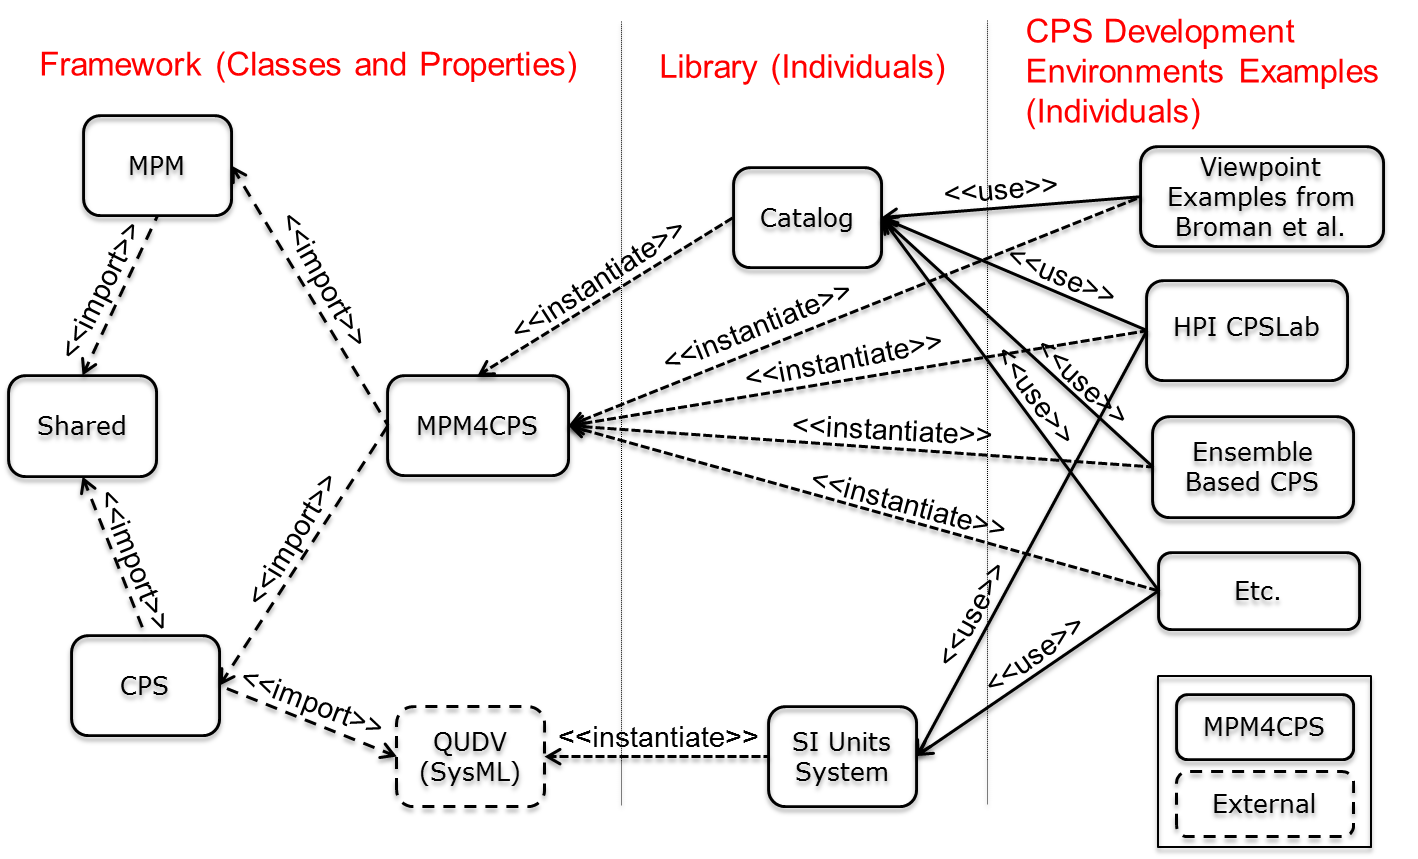
\includegraphics[width=\textwidth]{figures/ontology_structure.png}
\caption{Overview of the structure of the MPM4CPS ontology}
\label{fig:ontology_structure}
\end{figure}

In particular, figure \ref{fig:ontology_structure} provides an overview of the MPM4CPS ontology (shown in the first column).
It emphasises the unification of the two domains of Multi-Paradigm Modelling (MPM) and Cyber-Physical Systems (CPS), which are both foundations for this new emerging domain.

The figure further shows that the catalog (i.e. the contents of this document) is an instantiation of the MPM4CPS domain. The right column of the figure shows few examples of CPS developments that use multi-paradigm modelling. 
% and ``mega-models''. \COMMENT{ HG: Either we explain the role of MM here or leave the term out, or?}
These examples will not be presented in this report, but are elaborated on in the \emph{Framework to Relate / Combine Modeling Languages and Techniques} (see Deliverable D1.2 \cite{MPM4CPS-D1-2v1}).


\textbf{Automatic Catalog Creation:}
As stated, the individual formalisms, languages and tools of this catalog are based upon the MPM4CPS ontology. As one can easily imagine, many of the over 170 individual representatives of these concepts contain numerous connections to other individuals.
In general, a tight network of dependencies, compatibilities and other relations was discovered.
To fully exploit modern technologies, the catalog entries were entered directly into the ontology, so that the connections could be defined.
This catalog is generated directly from these ontology sources and thus shows one view of this ontology.
As an interactive, searchable and visual depiction of this data provides a more comprehensive view than this static generation, we are in the process of publishing the digital ontology alongside the final report.

 

% In figure \ref{fig:ontology_structure} the structure of the framework and its
% elements in form of the different ontologies and their dependencies are
% presented. The figure also includes the data for the next two chapters of this
% report.

% The first column depicts the framework and its ontologies as presented in the
% report on the Framework to Relate / Combine Modeling Languages and Techniques
% covered by deliverable D1.2 \cite{MPM4CPS-D1-2v1}.
% The Glossary of Terms for Cyber Physical Systems presented in chapter
% \ref{ch:glossary} of this report is extracted automatically from these
% ontologies and its contained concepts defining the framework.

% In the second column the catalog of modeling languages and tools that
% consists of indiciduals of the MPM4CPS ontology as covered later in chapter
% \ref{ch:catalog} is presented. It is automatically derived from these
% individuals such that the ontology and its instances can be kept consistent with
% minimal coordination efforts.

% In the third column, some examples for CPS development employing MPM in form of
% mega models are depicted. Those are presented in details in the report on
% the Framework to Relate / Combine Modeling Languages and Techniques covered by
% deliverable D1.2 \cite{MPM4CPS-D1-2v1}. As depicted, these examples employ
% individuals of the catalog of languages and tools listed in this report in
% chapter \ref{ch:catalog} and instantiate the classes of the MPM4CPS ontology.

% The  high-level framework presented in the form of framework ontologies  

% framework The work executed by WG1 highlights out by the 

\textbf{Usage of this catalog} This catalog serves as a valuable source of information and can be used as a reference to look up data about a large number of current modelling technologies and approaches.
The authors tried to add further references to each entry, such that formalisms show scientific references or sources of introduction material, and tool implementations are annotated with a hyperlink to the tool's webpage, where it can be downloaded from.

The catalog is structured as follows:
Chapter \ref{ch:catalog} presents the list of identified formalisms (Section \ref{sec:formalisms}), modelling languages (Section \ref{sec:languages}) and modelling tools (Section \ref{sec:tools}).
The list items each have a short description, extended by references and links to further resources to guide interested readers towards further information.
% The second chapter (Chapter \ref{ch:glossary}) captures a collection of the most common terms and abbreviations used in the modelling and cyber-physical systems domains in two tables.

% ========================================================
\begin{comment}

\todo[inline]{Original text below}

This report on the State-of-the-art on Current Formalisms used in Cyber-Physical
Systems Development of Working Group1 (WG1) on Foundations of the ICT COST
Action IC1404 Multi-Paradigm Modelling for Cyber-Physical Systems (MPM4CPS)
first presents a catalog of modeling languages and tools in chapter
\ref{ch:catalog}. Then a Glossary of Terms for Cyber Physical Systems is
presented in chapter \ref{ch:glossary}.

The work of WG1 revealed that the dependencies
between the framework targeted in deliverable D1.2 \cite{MPM4CPS-D1-2v1} and
this report was much more tight than initially expected. To avoid capturing some
content of this report  in a redundant form in the ontologies of the
framework, it was decided instead to  include relevant information in the
ontologies and extract it automatically from the ontologies for this report .


% Figure + description below

\begin{figure}[!htb]
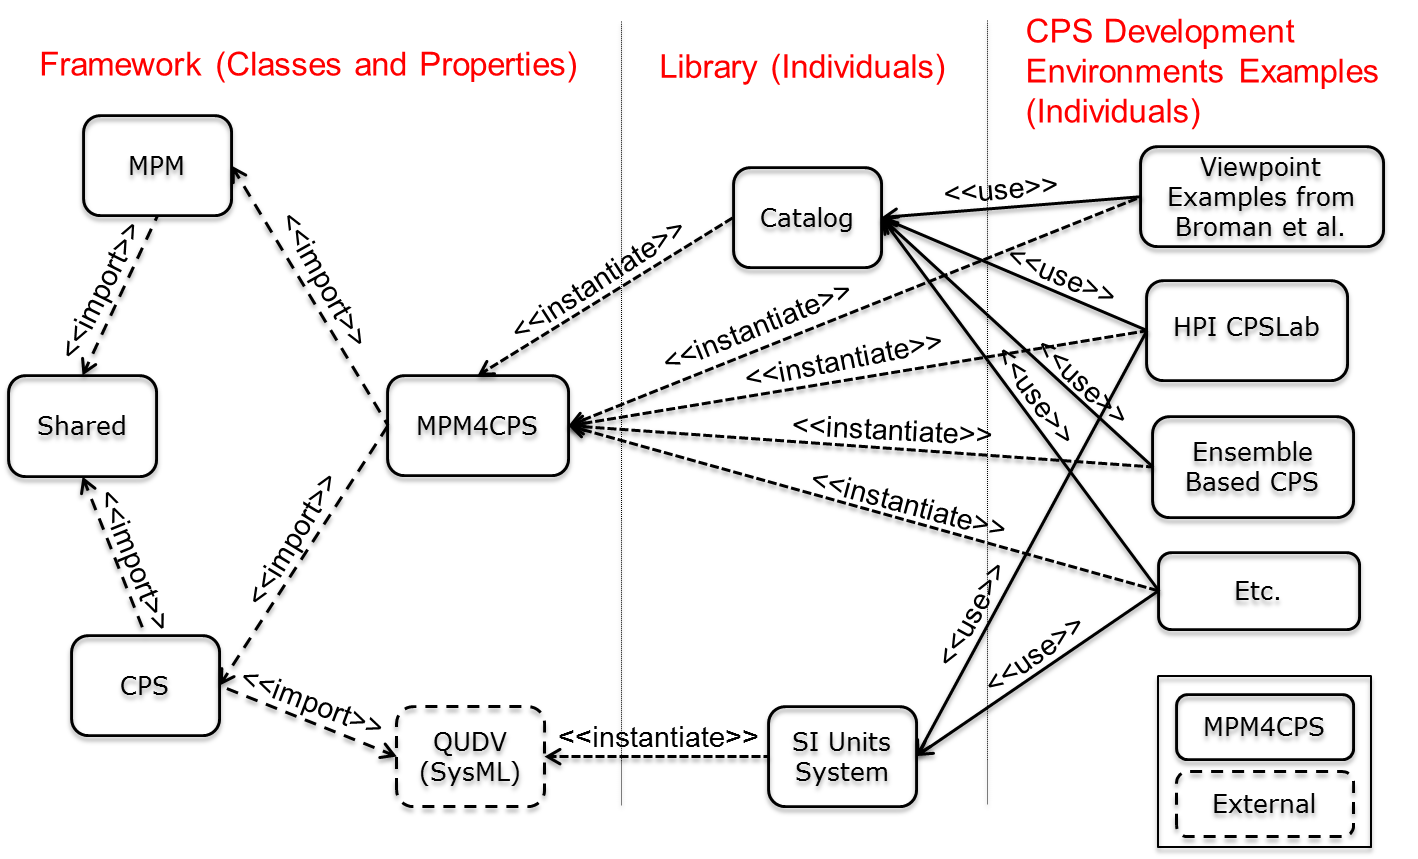
\includegraphics[width=\textwidth]{figures/ontology_structure.png}
\caption{Overview of the structure of the MPM4CPS ontology}
\label{fig:ontology_structure}
\end{figure}

In figure \ref{fig:ontology_structure} the structure of the framework and its
elements in form of the different ontologies and their dependencies are
presented. The figure also includes the data for the next two chapters of this
report.

The first column depicts the framework and its ontologies as presented in the
report on the Framework to Relate / Combine Modeling Languages and Techniques
covered by deliverable D1.2 \cite{MPM4CPS-D1-2v1}.
The Glossary of Terms for Cyber Physical Systems presented in chapter
\ref{ch:glossary} of this report is extracted automatically from these
ontologies and its contained concepts defining the framework.

In the second column the catalog of modeling languages and tools that
consists of indiciduals of the MPM4CPS ontology as covered later in chapter
\ref{ch:catalog} is presented. It is automatically derived from these
individuals such that the ontology and its instances can be kept consistent with
minimal coordination efforts.

In the third column, some examples for CPS development employing MPM in form of
mega models are depicted. Those are presented in details in the report on
the Framework to Relate / Combine Modeling Languages and Techniques covered by
deliverable D1.2 \cite{MPM4CPS-D1-2v1}. As depicted, these examples employ
individuals of the catalog of languages and tools listed in this report in
chapter \ref{ch:catalog} and instantiate the classes of the MPM4CPS ontology.
\end{comment}

% ========================================================
\chapter{Structured Catalog of Modelling Languages and Tools}
\label{ch:catalog}

The MPM4CPS domain merges concepts from multi-paradigm modelling (MPM) and applies them onto the development of cyber-physical systems.
As an extension of the well-known field of embedded systems development, the CPS discipline emerges from a widely studied field and thus builds upon its previous insights, development and modelling approaches and languages and tools.

On the other hand, CPS is a very recent field that embraces new ideas and modern paradigms.
These additions created diverging branches from existing standards and new target audiences and domain actors adopted multiple approaches: the result is that different stakeholders use different definitions for their approaches, with an evident dispersion of effort and a significant introduction of unnecessary conceptual entropy in the field in both literature and practice, that may be dominated by a substanding unifying approach suitable to keep beneficial diversity.
Consequently, MPM's aim is to further the diversity of topics by taking a very elastic approach and supporting generic (informal) definitions and merging the ``best formalisms, languages and tools'' for each point of view.
This stance however resulted in the creation of tools that were generated based on different
needs and from different points of view, spanning from small-scale, theoretical and hardware-centric  approaches to robust, practical, industrial and large-scale applications, and numerous other solutions inbetween.

This chaotic richness of tools is further founded by the
heterogeneity of users and backgrounds that are involved in the MPM4CPS processes.
MPM4CPS processes mirror the intrinsic complexity of
their systems and diversity of their users. These come from and
work in different domains, each bringing their specialised point of view,
heritage and methods of their respective domain.
Such methods belong to different phases of the
design, development and assessment cycle, and stem from various research fields,
with particular perspectives on the same problems and different views on similar
systems. As a result, specifications of tools are often divergent, even if not
contrasting, as they are driven by different purposes, towards different goals,
and on different methodological foundations.

This catalog aims to serve as a small collection of the most commonly employed tools, modelling languages and formalisms in the domain.
The catalog's initial purpose prescribed to capture current and actively used means to model CPS. However, it quickly became evident that the domain's vastness cannot be captured entirely in this document. Too many tools and languages have been developed and trialed in many experiments and evaluated on numerous case studies.
Instead, the decision was made to initially create a description of the most commonly known and used representatives of each category, and, in a second iteration, add representative usage reports and evaluations.

The catalog is by no means attempting to be complete or even exhaustive, as the described vastness and the speed of development, adaptation and change of the discipline renders such a goal unreachable.
What it does however is to serve as a reference for newcomers who wish to learn more about a particular formalism, language or tool.
The catalog further provides references to additional information resources such as experience reports, case studies and analyses.

Catalog entries has been selected by experts in their respective fields and participants of the MPM4CPS's WG1 on Foundations. 
Collectively, they serve as a current snapshot of the main and most important concepts, but -- similar to other lexica and reference sources -- has to be extended, revisited and updated in regular intervals (as intended by the members of WG1).

\section{Catalog Structure}\label{sec:CatalogStructure}
The structure of the catalog is inspired by the framework proposed by~\cite{Broman2012}, which distinguishes between viewpoints, formalisms, and languages and tools.
It defines that stakeholders have viewpoints which are expressed using formalisms.
As formalisms are mathematical structures (i.e. without a concrete syntax), they require languages and tools that implement them.
Figure \ref{fig:broman} depicts this framework visually. 
Evidently, modern tools often support several languages, and each language can merge several formalisms.
For example, Papyrus is a tool that supports the creation of different Unified Modeling Language (UML) diagram types such as \textit{class diagrams}, \textit{sequence diagrams}, etc.
Each diagram is based upon a different formalism.

\begin{figure}[!htb]
\centering
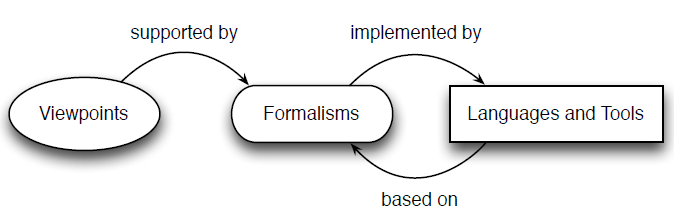
\includegraphics[width=0.7\textwidth]{figures/fw_viewpoints_bronan.png}
\caption{Framework for Viewpoints, Formalisms, Languages and Tools (from~\cite{Broman2012})}
\label{fig:broman}
\end{figure}

The catalog lists its entries in a pre-defined order, starting from the most theoretical (formalisms) to the most practical (tools).
In some situations, the classification of individual entries is not easily possible.
For example, \textit{Petri nets} are a family of formalisms that are well-suited for the expression of concurrency. 
There are various ``flavours'' of Petri nets that allow the expression of different systems.
As they are closely related though, the catalog authors choose to list them as individual formalisms, even though one might argue that \textit{Colored Petri nets} are a formalism by themselves.
Another issue arises with the classification of Petri nets, as, when they were introduced, Petri nets were equipped with a visual notation syntax, which nowadays is used interchangeably with the mathematical formalism.
This catalog thus lists two different entries for ``Petri nets'' (i.e. the formalism) and ``Petri nets diagram'' (i.e. its graphical syntax). 
The reason behind this is that there exists for example the \textit{PNML} (Petri Net Markup Language) format, which is a common exchange format for Petri net diagrams that can be easily read and written by tools.
It is thus another language (with a concrete, textual syntax) for the Petri nets formalism.
Finally, the tools section (Section \ref{sec:tools}) provides a list of tools that can be used to create, edit, and interact with models. 
For example, the section contains an entry for \textit{StrataGEM}, a common tool for the model-checking of concurrent models such as Petri nets.

\begin{comment}

\section{Introduction}

A number of different tools is available that support multiparadigm modeling
and/or CPS modeling, at different maturity levels, designed by academia or
industry. This richness is quite natural, for different reasons. 

As first, CPS is a recent field, with no established standards and with
different actors, each of which adopts a slightly different definition and a
different approach for the topic: while multiparadigm modeling embraces a very
wide spectrum of different topics, and actually has a very elastic and generic
(informal) definition: the result is that tools were generated under different
needs and from different directions, as the field spans from very theoretical,
foundational approaches to very practical, application oriented approaches.

As second, this chaotic richness of tools is easily explained by the
heterogeneity of users and backgrounds that are involved in the processes that
are in the scope of interest of MPM4CPS that mirrors the intrinsic complexity of
the systems that are in the scope of interest of MPM4CPS. They come from and
work in different domains, each bringing the specialistic point of view,
heritage and methods of their domain, they belong to different phases of the
design, development and assessment cycle, or from different research fields,
with different perspectives on the same problems and different views on the same
systems. As a result, specifications of tools are often divergent, even if not
contrasting, as they are driven by different purposes, towards different goals,
and on different methodological foundations.

In this chapter a catalogue of tools is presented, with a classification that is
derived from the ontology. Some of the tools are released as commercial
software in support of different applications, others are pure experimental
tools devoted to support research in language engineering or model engineering.
For each tool the main points have been resumed and classified, in order to
provide a comprehensive support for candidate users and to guide them in
exploring the offer to find the best match to their needs.

The structure of the catalog is inspired from the framework proposed by~\cite{Broman2012} (see figure \ref{fig:broman}) where modeling languages and tools may be based on / support a set of formalisms and conversely, formalisms may be implemented by languages and tools. Therefore, the catalog proposed three top level lists for languages, tools and formalisms with subsections for referencing the related elements via the aforementioned relations. In addition, for each element of the catalog a set of references is provided.

\begin{figure}[!htb]
\centering
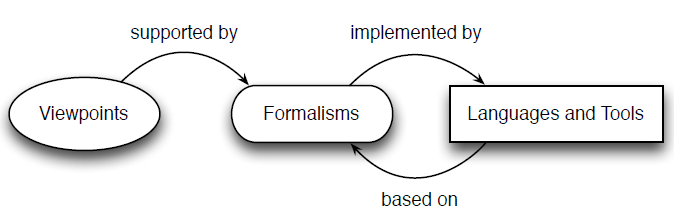
\includegraphics[width=0.7\textwidth]{figures/fw_viewpoints_bronan.png}
\caption{Framework for Viewpoints, Formalisms, Languages and Tools (from~\cite{Broman2012})}
\label{fig:broman}
\end{figure}
\end{comment}

%\todo{???: should we add %here a copy of the %figure or a diagram from %the ontology?\\
%Holger: yes. I think %this would be very %helpful.
%}

\section{Formalisms}
\label{sec:formalisms}

The following subsections present the most commonly used formalisms for cyber-physical systems development.

\subsection{Automata-based Formalisms}

\subsubsection{Abstract State Machines}
\label{subsecF:AbstractStateMachines}
\index{Abstract State Machines}
\index{Formalisms!Abstract State Machines}
\authors{Stefan Klikovits}


Abstract state machines are a formalism that model the states and their transitions.
ASM are an extension of Finite State Machines (FSM) and allow the representation of states as arbitrary data types. The formalism aims to bridge the gap between human-readable, easily understandable specifications and machine-executable code.
Application areas of ASM are for example the modelling and verification of programming languages, protocols, embedded systems, etc.

\textbf{Implementing Languages}

Abstract State Machines is a formalism for the following languages:
\begin{itemize}
	\item AADL (see section \ref{subsecL:AADL})
	\item AsmL (see section \ref{subsecL:AsmL})
	\item AsmetaL (see section \ref{subsecL:AsmetaL})
	\item Gofer (see section \ref{subsecL:Gofer})
\end{itemize}


\cpsUsage{Usage for CPS Development}

\todoAuthors{Provide ``mpm4cps:usage:cps'' annotation assertion in ontology}


\textbf{References}
\begin{itemize}
	
\item \bibentry{Borger1999}
	
\item \bibentry{Borger2005}
	
\item \bibentry{Borger2003}
\end{itemize}



\subsubsection{Cellular Automata}
\label{subsecF:CellularAutomata}
\index{Cellular Automata}
\index{Formalisms!Cellular Automata}
\authors{Stefan Klikovits}

\reviewers{Florin Leon}

Cellular Automata (CA) is a popular formalism for the idealisation of physical systems.
A system consists of an n-dimensional lattice of uniform ``cells''. 
Each cell is an automaton, whose behaviour (discrete state transitions) is defined by its own state, and the states of cells in its ``neighbourhood'' (the cells with a certain distance, e.g. direct neighbours).
The transitions of all CA in the system are executed at the same time.
By representing automaton behaviour using relatively simple rules, highly complex system behaviour can be expressed. Since their introduction in the 1950ies, cellular automata had various waves of popularity.
Recently they are used to model and study emergent behaviour in very large and highly complex systems consisting of uniform units.
One of the most popular CA case studies is Conway's ``Game of Life''.

\textbf{Implementing Languages}

None


\cpsUsage{Usage for CPS Development}

\beginCpsUsage{itemize}

\itemCpsUsage \bibentryCpsUsage{H2015}

\itemCpsUsage \bibentryCpsUsage{Z2013}

\itemCpsUsage \bibentryCpsUsage{THVP2016}
\bendCpsUsage{itemize}


\textbf{References}
\begin{itemize}
	
\item \bibentry{Chopard2012}
	
\item \bibentry{Athanassopoulos2012}
	
\item \bibentry{Cellular-Automata-website}
\end{itemize}
\subsubsection{Hybrid Automata-based Formalisms}

\subsubsection{Hybrid Automata}
\label{subsecF:HybridAutomata}
\index{Hybrid Automata}
\index{Formalisms!Hybrid Automata}
\authors{Eva Navarro}


A finite state automaton is a computational abstraction of the transitions of a system between discrete states or locations (on and off, for instance). A hybrid automaton, additionally, considers dynamical evolution over time in each location. This dynamical evolution is represented by a dynamical system. Depending on the nature of the dynamics of this system, different types of hybrid automata are defined; the main ones are explained as follows. Hybrid automata is one of the many existing modelling frameworks of hybrid systems.

\textbf{Implementing Languages}

Hybrid Automata is a formalism for the following languages:
\begin{itemize}
	\item Stateflow Language (see section \ref{subsecL:StateFlowLanguage})
	\item Scilab Language (see section \ref{subsecL:ScilabLanguage})
	\item PyDSTool Language (see section \ref{subsecL:PyDSToolLanguage})
	\item NuSMV Language (see section \ref{subsecL:NuSMVLanguage})
	\item Ptolemy Language (see section \ref{subsecL:PtolemyLanguage})
	\item Modelica (see section \ref{subsecL:Modelica})
\end{itemize}


\cpsUsage{Usage for CPS Development}

\todoAuthors{Provide ``mpm4cps:usage:cps'' annotation assertion in ontology}


\textbf{References}
\begin{itemize}
	
\item \bibentry{Lygeros2010}
	
\item \bibentry{Abate2010}
\end{itemize}



\subsubsection{I/O Hybrid Automata (Hybrid Input/Output Automata)}
\label{subsecF:HybridI/OHybridAutomata}
\index{I/O Hybrid Automata}
\index{Formalisms!I/O Hybrid Automata}
\authors{Stefan Klikovits}

\reviewers{Eva Navarro}

I/O hybrid automata are a class of hybrid automata that include asynchronous distributed system components. The automaton's transitions are annotated with input actions and output actions, which are executed at when triggering a transition.

\textbf{Implementing Languages}

None


\cpsUsage{Usage for CPS Development}

\todoAuthors{Provide ``mpm4cps:usage:cps'' annotation assertion in ontology}


\textbf{References}
\begin{itemize}
	
\item \bibentry{Lynch1989}
	
\item \bibentry{Lynch2003}
\end{itemize}



\subsubsection{Linear Hybrid Automata}
\label{subsecF:HybridAutomataLinear}
\index{Linear Hybrid Automata}
\index{Formalisms!Linear Hybrid Automata}
\authors{Eva Navarro}


A linear hybrid automaton is a hybrid automaton where the dynamical system within each location or discrete state is linear.

\textbf{Implementing Languages}

Linear Hybrid Automata is a formalism for the following languages:
\begin{itemize}
	\item Stateflow Language (see section \ref{subsecL:StateFlowLanguage})
	\item Scilab Language (see section \ref{subsecL:ScilabLanguage})
	\item PyDSTool Language (see section \ref{subsecL:PyDSToolLanguage})
	\item NuSMV Language (see section \ref{subsecL:NuSMVLanguage})
	\item Ptolemy Language (see section \ref{subsecL:PtolemyLanguage})
	\item Modelica (see section \ref{subsecL:Modelica})
\end{itemize}


\cpsUsage{Usage for CPS Development}

\todoAuthors{Provide ``mpm4cps:usage:cps'' annotation assertion in ontology}


\textbf{References}
\begin{itemize}
	
\item \bibentry{Lygeros2010}
	
\item \bibentry{Abate2010}
\end{itemize}



\subsubsection{Non-Linear Hybrid Automata}
\label{subsecF:HybridAutomataNonLinear}
\index{Non-Linear Hybrid Automata}
\index{Formalisms!Non-Linear Hybrid Automata}
\authors{Eva Navarro}


A nonlinear hybrid automaton is a hybrid automaton where the dynamical system within each location or discrete state is nonlinear. The studies on nonlinear hybrid automata are much less than in linear hybrid automata due to the complexity of the dynamical behaviours involved.

\textbf{Implementing Languages}

Non-Linear Hybrid Automata is a formalism for the following languages:
\begin{itemize}
	\item Stateflow Language (see section \ref{subsecL:StateFlowLanguage})
	\item Scilab Language (see section \ref{subsecL:ScilabLanguage})
	\item PyDSTool Language (see section \ref{subsecL:PyDSToolLanguage})
	\item NuSMV Language (see section \ref{subsecL:NuSMVLanguage})
	\item Ptolemy Language (see section \ref{subsecL:PtolemyLanguage})
	\item Modelica (see section \ref{subsecL:Modelica})
\end{itemize}


\cpsUsage{Usage for CPS Development}

\todoAuthors{Provide ``mpm4cps:usage:cps'' annotation assertion in ontology}


\textbf{References}
\begin{itemize}
	
\item \bibentry{Lygeros2010}
	
\item \bibentry{Abate2010}
\end{itemize}



\subsubsection{PTAs (Priced/Probabilistic Timed Automata)}
\label{subsecF:PTAs}
\index{PTAs}
\index{Formalisms!PTAs}
\authors{Stefan Klikovits}

\reviewers{Moussa Amrani, Eva Navarro}

A priced timed automaton is a timed automaton where transitions and locations are annotated with real-valued costs and cost rates, respectively. The global cost increases according to the cost rate of the current location and ``jumps'' when taking a transition (according to the cost annotation of the transition).

Note, that the cost rate of each location can be different, but cannot be negative.

\textbf{Implementing Languages}

PTAs is a formalism for the following languages:
\begin{itemize}
	\item PRISM Language (see section \ref{subsecL:PRISMLanguage})
\end{itemize}


\cpsUsage{Usage for CPS Development}

\todoAuthors{Provide ``mpm4cps:usage:cps'' annotation assertion in ontology}


\textbf{References}
\begin{itemize}
	
\item \bibentry{Behrmann2005}
\end{itemize}



\subsubsection{Stochastic Hybrid Automata}
\label{subsecF:HybridAutomataStochastic}
\index{Stochastic Hybrid Automata}
\index{Formalisms!Stochastic Hybrid Automata}
\authors{Eva Navarro}


A stochastic hybrid automaton is a class of non-deterministic hybrid automaton where uncertainty is introduced  in the system evolution and the control inputs. The main differences with respect to a hybrid automaton are: 1) the initial state (initial discrete location and initial continuous state vector) is chosen at random, 2) the continuous state evolves following stochastic differential equations, 3) there are two types of discrete transitions between locations that give rise to two types of guards conditions: forced transitions and spontaneous transitions; spontaneous transitions are triggered by stochastic events.

\textbf{Implementing Languages}

Stochastic Hybrid Automata is a formalism for the following languages:
\begin{itemize}
	\item Stateflow Language (see section \ref{subsecL:StateFlowLanguage})
	\item Scilab Language (see section \ref{subsecL:ScilabLanguage})
	\item PyDSTool Language (see section \ref{subsecL:PyDSToolLanguage})
	\item Simulink Language (see section \ref{subsecL:SimulinkLanguage})
	\item Ptolemy Language (see section \ref{subsecL:PtolemyLanguage})
	\item Modelica (see section \ref{subsecL:Modelica})
\end{itemize}


\cpsUsage{Usage for CPS Development}

\todoAuthors{Provide ``mpm4cps:usage:cps'' annotation assertion in ontology}


\textbf{References}
\begin{itemize}
	
\item \bibentry{Lygeros2010}
	
\item \bibentry{Abate2010}
\end{itemize}



\subsubsection{Stochastic Timed Automata}
\label{subsecF:TimedAutomataStochastic}
\index{Stochastic Timed Automata}
\index{Formalisms!Stochastic Timed Automata}
\authors{Stefan Klikovits}

\reviewers{Moussa Amrani, Eva Navarro}

Stochastic timed automata extend the TA formalism by adding probabilistic concepts, which allow the stochastic selection of enabled transitions and delays (i.e. time spent within a location).

\textbf{Implementing Languages}

Stochastic Timed Automata is a formalism for the following languages:
\begin{itemize}
	\item UPPAAL SMC Language (see section \ref{subsecL:UPPAALSMCSpecificationLanguage})
\end{itemize}


\cpsUsage{Usage for CPS Development}

\todoAuthors{Provide ``mpm4cps:usage:cps'' annotation assertion in ontology}


\textbf{References}
\begin{itemize}
	
\item \bibentry{bertrand2014}
\end{itemize}



\subsubsection{Timed Automata}
\label{subsecF:TimedAutomata}
\index{Timed Automata}
\index{Formalisms!Timed Automata}
\authors{Stefan Klikovits}

\reviewers{Moussa Amrani, Eva Navarro}

Timed automata (TA) is a formalism that merges the concepts of discrete automata theory with the continuous evolution of variables (``clocks''). 
Each clock progressively increases its value at a constant rate (i.e. 1).
Transition guards can be defined by comparing the clocks' values to constants.
Further, each clock can be reset to zero when firing transitions.

Timed automata can be seen as a specialisation of hybrid automata, where all clock rates are constant and equal, transition guards only allow linear comparisons of clocks and transitions (hybrid automata jumps) can only reset clock values to zero.

Many extensions of timed automata have been proposed, such as stopwatch automata (the rate can be temporarily set to 0), and hourglass automata (the clocks' rate can be reversed to -1).

\textbf{Implementing Languages}

Timed Automata is a formalism for the following languages:
\begin{itemize}
	\item HyTech Language (see section \ref{subsecL:HyTechLanguage})
	\item Kronos Language (see section \ref{subsecL:KronosLanguage})
	\item UPPAAL Language (see section \ref{subsecL:UPPAALRequirementSpecificationLanguage})
\end{itemize}


\cpsUsage{Usage for CPS Development}

\todoAuthors{Provide ``mpm4cps:usage:cps'' annotation assertion in ontology}


\textbf{References}
\begin{itemize}
	
\item \bibentry{Alur1994}
	
\item \bibentry{Cassez2000}
	
\item \bibentry{Bengtsson2004}
	
\item \bibentry{Osada2014}
\end{itemize}



\subsubsection{Timed I/O Automata (Timed Input/Output Automata)}
\label{subsecF:TimedI/OAutomata}
\index{Timed I/O Automata}
\index{Formalisms!Timed I/O Automata}
\authors{Stefan Klikovits}


The Timed I/O Automata formalism is an extension of interface automata to include timing information. The automaton's transitions are annotated with input actions and output actions, which are executed at when triggering a transition.

\textbf{Implementing Languages}

None


\cpsUsage{Usage for CPS Development}

\todoAuthors{Provide ``mpm4cps:usage:cps'' annotation assertion in ontology}


\textbf{References}
\begin{itemize}
	
\item \bibentry{Kaynar2010}
	
\item \bibentry{David2010}
\end{itemize}

\subsection{Flow-based Formalisms}

\subsubsection{Data Flow}
\label{subsecF:DataFlow}
\index{Data Flow}
\index{Formalisms!Data Flow}
\authors{Etienne Borde, Stefan Klikovits}


DataFlow describes an computation model that resembles a graph. Each node represents a function (usually called actor) and each arc represents a communication channel between two functions. All the inputs of a function must be present to start its execution. In synchronous dataflow modelling the ``synchronous hypothesis'' states that the computation of each function and the communication between two functions is infinitely fast (or instantaneous). 

Given this hypothesis, SDF provides a sound model of computation with predictable performance, properties verification methods (liveness, deadlock freedom), and predictable buffering.

The practical approach relies on the fact that the computation of a node starts only when the execution of all its predecessors is finished. This requires that the graph topology is loop-free. Since SDF are usually executed in periodic tasks, the synchronous hypothesis is usually considered to be verified as the worst case response time of the graph is smaller than the task's period.

This type of model is well-suited to digital signal processing and communications systems which often process an endless supply of data. It has been successfully applied in the domain of safety critical embedded systems. It has also been characterised or extended into homogeneous data flow graphs, cyclo-static data flow graphs, scenario-aware data flow graphs, affine data flow graphs.

\textbf{Implementing Languages}

Data Flow is a formalism for the following languages:
\begin{itemize}
	\item AADL (see section \ref{subsecL:AADL})
	\item Lustre (see section \ref{subsecL:Lustre})
	\item Z\'elus (see section \ref{subsecL:Zelus})
	\item Signal (see section \ref{subsecL:Signal})
\end{itemize}


\cpsUsage{Usage for CPS Development}

\todoAuthors{Provide ``mpm4cps:usage:cps'' annotation assertion in ontology}


\textbf{References}
\begin{itemize}
	
\item \bibentry{Murthy2002}
\end{itemize}



\subsubsection{HyFlow (Hybrid Flow System Specification)}
\label{subsecF:HyFlow}
\index{HyFlow}
\index{Formalisms!HyFlow}
\authors{Fernando Barros}


HyFlow provides a formal description of dynamic topology hybrid systems \cite{Barros:2003:DSM}. This formalism can model systems that exhibit both continuous and discrete behaviors while relying on a digital computer representation. HyFlow supports multisampling as a first order operator, enabling both time and component varying sampling, making it suitable for representing sampled-based systems, like digital controllers and filters. HyFlow provides also an extrapolation operator that enables an error free representation of continuous signals. Multisampling can be used for achieving an explicit representation of asynchronous adaptive stepsize differential equations integrators \cite{Barros-2018:Geometric}. HyFlow provides an integrative framework for combing models expressed in different modeling paradigms. In particular, fluid stochastic Petri-nets \cite{Barros-2015:FSPN} and geometric integrators \cite{Barros-2018:Geometric}, for example, can be  represented in the HyFlow formalism, enabling its seamless integration with other HyFlow models. HyFlow sampling provides an expressive operator for making the connection of computer-based systems with real-time systems, since sampling is, in many cases, the most convenient operator to interact with continuous signals. HyFlow supports modular and hierarchical models providing deterministic semantics for model composition and co-simulation \cite{Barros:2008:SDS}.

\textbf{Implementing Languages}

None


\cpsUsage{Usage for CPS Development}

\todoAuthors{Provide ``mpm4cps:usage:cps'' annotation assertion in ontology}


\textbf{References}
\begin{itemize}
	
\item \bibentry{Barros-2018:Geometric}
	
\item \bibentry{Barros:2008:SDS}
	
\item \bibentry{Barros:2003:DSM}
	
\item \bibentry{Barros-2015:FSPN}
\end{itemize}

\subsection{Logic-based Formalisms}

\subsubsection{CTL (Computation Tree Logic)}
\label{subsecF:CTL}
\index{CTL}
\index{Formalisms!CTL}
\authors{Stefan Klikovits}


CTL is a branching-time temporal logic that allows the analysis of tree-like structures.
It allows the analysis of various future evolution paths to answer questions whether there is a possibility that an event might or will happen.
Various model checkers exist that allow the verification of the reachability and liveness of certain events (or event sequences).

\textbf{Implementing Languages}

CTL is a formalism for the following languages:
\begin{itemize}
	\item NuSMV Language (see section \ref{subsecL:NuSMVLanguage})
\end{itemize}


\cpsUsage{Usage for CPS Development}

\todoAuthors{Provide ``mpm4cps:usage:cps'' annotation assertion in ontology}


\textbf{References}
\begin{itemize}
	
\item \bibentry{Huth2004}
\end{itemize}



\subsubsection{First Order Logic}
\label{subsecF:FirstOrderLogic}
\index{First Order Logic}
\index{Formalisms!First Order Logic}
\authors{Moussa Amrani}

\reviewers{Florin Leon, Stefan Klikovits}

First-Order Logic (\textsc{FOL}, also ``First-Order Predicate Calculus'') is a logical formalism constituted of terms and formulas. A term is either a variable, a function symbol or a predicate symbol. A formula is constituted of formulas built over terms combined with the usual Boolean operators (negation, conjunction and so on) and both existential and universal quantifiers. First-Order Logic formulas are interpreted on a (finite) domain, and possess a sound and complete calculus, making it automatable for reasoning \cite{B:Kleene:2002}.

\textbf{Implementing Languages}

First Order Logic is a formalism for the following languages:
\begin{itemize}
	\item SMT-LIB (see section \ref{subsecL:SMTLIBLanguage})
\end{itemize}


\cpsUsage{Usage for CPS Development}

\beginCpsUsage{itemize}

\itemCpsUsage \bibentryCpsUsage{P2016}
\bendCpsUsage{itemize}


\textbf{References}
\begin{itemize}
	
\item \bibentry{B:Kleene:2002}
\end{itemize}



\subsubsection{Linear Temporal Logic}
\label{subsecF:LTL}
\index{Linear Temporal Logic}
\index{Formalisms!Linear Temporal Logic}
\authors{Stefan Klikovits}


LTL is a representative of the family of temporal logics that analyses the future evolution of paths. It allows the testing of one individual branch (as opposed to CTL).

\textbf{Implementing Languages}

Linear Temporal Logic is a formalism for the following languages:
\begin{itemize}
	\item Kronos Language (see section \ref{subsecL:KronosLanguage})
	\item PROMISE Language (see section \ref{subsecL:PROMISEDSL})
	\item PSC (see section \ref{subsecL:PSC})
\end{itemize}


\cpsUsage{Usage for CPS Development}

\todoAuthors{Provide ``mpm4cps:usage:cps'' annotation assertion in ontology}


\textbf{References}
\begin{itemize}
	
\item \bibentry{Huth2000}
\end{itemize}



\subsubsection{Temporal Logic}
\label{subsecF:TemporalLogic}
\index{Temporal Logic}
\index{Formalisms!Temporal Logic}
\authors{Stefan Klikovits}


A temporal logic (also tense logic) system is a formal mathematical system that allows the reasoning about terms and their truth value related to time. It is an extension of first-order logic and allows the expression of statements such as "I always model CPS", "I will eventually model a CPS'" and "I will not model CPS until I find a good formalism". 

Temporal logic is frequently used in formal verification, where it is used to formally express requirements (e.g. the reaching of a certain state). Popular temporal logic systems are for example the linear temporal logic (LTL), computation tree logic (CTL) and Hennessy-Milner logic (HML).

\textbf{Implementing Languages}

Temporal Logic is a formalism for the following languages:
\begin{itemize}
	\item NuSMV Language (see section \ref{subsecL:NuSMVLanguage})
\end{itemize}


\cpsUsage{Usage for CPS Development}

\todoAuthors{Provide ``mpm4cps:usage:cps'' annotation assertion in ontology}


\textbf{References}
\begin{itemize}
	
\item \bibentry{Pnueli1977}
\end{itemize}

\subsection{Petri Net-based Formalisms}

\subsubsection{High Level Petri Nets}
\label{subsecF:PetriNetsHighLevel}
\index{High Level Petri Nets}
\index{Formalisms!High Level Petri Nets}
\authors{Didier Buchs}


This large class rely on another modeling framework devoted to the description of the data attached to the tokens, and the expression that must be assigned to arcs describing the computation that must be done for satisfying the pre and post conditions. Among several dialect of these class we can cite algebraic Petri Nets and coloured Petri Nets.

\textbf{Implementing Languages}

High Level Petri Nets is a formalism for the following languages:
\begin{itemize}
	\item PNML (see section \ref{subsecL:PNML})
	\item Petri Net Diagram (see section \ref{subsecL:PetriNetDiagram})
\end{itemize}


\cpsUsage{Usage for CPS Development}

\todoAuthors{Provide ``mpm4cps:usage:cps'' annotation assertion in ontology}


\textbf{References}

\todoAuthors{Provide ``rdfs:seeAlso'' annotation in ontology}



\subsubsection{Petri Net (Place Transition Nets)}
\label{subsecF:PetriNet}
\index{Petri Net}
\index{Formalisms!Petri Net}
\authors{Didier Buchs}

\reviewers{Mauro Iacono, Stefan Klikovits}

A Petri net (also known as a place/transition net or P/T net) is a formalism for the description of dynamic discrete systems. It is particularly suited to the modeling of systems where distribution, concurrency and non-determinism is important to discribe and analyze. The mathematical foundation of Petri nets has led to several development to make possible complex analsis of systems decribed by Petri nets. A Petri net is a directed bipartite graph, in which the nodes represent transitions (i.e. events that may occur, represented by bars or black rectangles) and places (i.e. conditions or ressources, represented by circles). The directed arcs describe which places are pre- and/or postconditions for which transitions (signified by arrows).  Petri nets were invented, according to some sources, in August 1939 by Carl Adam Petri at the age of 13 for the purpose of describing chemical processes.

Petri nets offer a graphical notation which is of particular interest to the engineer analyzing systems, natural pattern of design are existing in Petri nets such as causality, choice, independence and ressource management.

There are attempts for several formalisms Like UML activity diagrams, Business Process Model and Notation and EPCs to have semantics in term of translation into Petri nets. These translations have been used to provide a precise semantics to such formalisms as well as to  develop tools for their simulation and analysis.

It has been observed that in practice Petri Nets lack of modeling power for some modeling dimensions such as: timing aspects, data structures, stochastic processes and event priority. In general the formal analysis tool need different techniques if new modeling dimensions are introduced. So tools are generally different and adapted to the specific extensions.

Petri Nets have several extensions which are concretised in the following formalisms, it must be noted that the computing power of such extensions can change according to the new concepts introduced in the notations (i.e. time) and then the analysability of the models is sometime much more difficult or limited to extention with finiteness assumptions (i.e. high level nets):

\textbf{Implementing Languages}

Petri Net is a formalism for the following languages:
\begin{itemize}
	\item PNML (see section \ref{subsecL:PNML})
	\item Petri Net Diagram (see section \ref{subsecL:PetriNetDiagram})
	\item FIACRE (see section \ref{subsecL:FIACRE})
\end{itemize}


\cpsUsage{Usage for CPS Development}

\todoAuthors{Provide ``mpm4cps:usage:cps'' annotation assertion in ontology}


\textbf{References}
\begin{itemize}
	
\item CPN preserve useful properties of Petri nets and at the same time extend initial formalism to allow the distinction between tokens.
Coloured Petri Nets allow tokens to have a data value attached to them. This attached data value is called token color. 

\url{https://en.wikipedia.org/wiki/Coloured_Petri_net}
\end{itemize}



\subsubsection{Petri Nets with Priority}
\label{subsecF:PetriNetsPrioritised}
\index{Petri Nets with Priority}
\index{Formalisms!Petri Nets with Priority}
\authors{Didier Buchs}


This simple extension bring new semantics to the transition firing in order to solve conflict. Depending on the variant it can lead to more powerful models which are Turing complete.

\textbf{Implementing Languages}

Petri Nets with Priority is a formalism for the following languages:
\begin{itemize}
	\item PNML (see section \ref{subsecL:PNML})
	\item Petri Net Diagram (see section \ref{subsecL:PetriNetDiagram})
\end{itemize}


\cpsUsage{Usage for CPS Development}

\todoAuthors{Provide ``mpm4cps:usage:cps'' annotation assertion in ontology}


\textbf{References}

\todoAuthors{Provide ``rdfs:seeAlso'' annotation in ontology}



\subsubsection{Stochastic Petri Nets}
\label{subsecF:PetriNetsStochastic}
\index{Stochastic Petri Nets}
\index{Formalisms!Stochastic Petri Nets}
\authors{Didier Buchs}


The firing of transitions follows a probabilistic distibution on time duration or frequency of transitions firing when there is a conflict.

\textbf{Implementing Languages}

Stochastic Petri Nets is a formalism for the following languages:
\begin{itemize}
	\item PNML (see section \ref{subsecL:PNML})
	\item Petri Net Diagram (see section \ref{subsecL:PetriNetDiagram})
\end{itemize}


\cpsUsage{Usage for CPS Development}

\todoAuthors{Provide ``mpm4cps:usage:cps'' annotation assertion in ontology}


\textbf{References}

\todoAuthors{Provide ``rdfs:seeAlso'' annotation in ontology}



\subsubsection{Timed Petri Nets}
\label{subsecF:PetriNetsTimed}
\index{Timed Petri Nets}
\index{Formalisms!Timed Petri Nets}
\authors{Didier Buchs}


Timed Petri Nets introduce time as a modeling dimension. This is reflected in aspect such as transition duration or possible interval for firing transitions. Generally these classes bring new problems for analysing them, in particular the time-line which has no limit in the future and the density of the time.

\textbf{Implementing Languages}

Timed Petri Nets is a formalism for the following languages:
\begin{itemize}
	\item PNML (see section \ref{subsecL:PNML})
	\item Petri Net Diagram (see section \ref{subsecL:PetriNetDiagram})
	\item FIACRE (see section \ref{subsecL:FIACRE})
\end{itemize}


\cpsUsage{Usage for CPS Development}

\todoAuthors{Provide ``mpm4cps:usage:cps'' annotation assertion in ontology}


\textbf{References}
\begin{itemize}
	
\item \bibentry{Abdulla2001}
	
\item \bibentry{Berthomieu1991}
\end{itemize}

\subsection{Other Formalisms}

\subsubsection{Bayesian Networks}
\label{subsecF:BayesianNetworks}
\index{Bayesian Networks}
\index{Formalisms!Bayesian Networks}
\authors{Stefan Klikovits}

\reviewers{Florin Leon}

Bayesian networks are a formalism that establishes a probabilistic graph model.
The vertices of the directed acyclic graph represent random variable probabilities and edges between them represent probabilistic dependencies. Hence each vertex depends on its predecessors.
Bayesian networks are well-suited to create simple computations for models with many variables.
They can further be used to encode hypotheses, hypotheses, beliefs, and latent variables.

\textbf{Implementing Languages}

None


\cpsUsage{Usage for CPS Development}

\beginCpsUsage{itemize}

\itemCpsUsage \bibentryCpsUsage{POC2011}

\itemCpsUsage \bibentryCpsUsage{KST2014}

\itemCpsUsage \bibentryCpsUsage{N2013}
\bendCpsUsage{itemize}


\textbf{References}
\begin{itemize}
	
\item \bibentry{Niedermayer2008}
\end{itemize}



\subsubsection{Bond Graphs}
\label{subsecF:BondGraphs}
\index{Bond Graphs}
\index{Formalisms!Bond Graphs}
\authors{Stefan Klikovits}


Bond graphs focus on the modelling of energy flows. The formalism recognises that different energy domains (electrical, hydraulic, mechanical) can be similarly represented and that the dual forces of "flow" (e.g. current, velocity) and ``effort'' (e.g. voltage, force) in combination create power. Bond graphs models represent idealised energy flows. Usually the same notation is used for all energy domains and domains switches are modelled using  e.g. gyrators and transformers. The formalism is actively used in engineering domains where it serves good purpose of prototyping the energy flow within a system.

\textbf{Implementing Languages}

Bond Graphs is a formalism for the following languages:
\begin{itemize}
	\item 20-sim Bond Graph (see section \ref{subsecL:TwentySimBondGraph})
\end{itemize}


\cpsUsage{Usage for CPS Development}

\todoAuthors{Provide ``mpm4cps:usage:cps'' annotation assertion in ontology}


\textbf{References}
\begin{itemize}
	
\item \bibentry{Martyn1961}
	
\item \bibentry{Broenink1999}
\end{itemize}



\subsubsection{Causal Block Diagrams}
\label{subsecF:CausalBlockDiagrams}
\index{Causal Block Diagrams}
\index{Formalisms!Causal Block Diagrams}
\authors{Stefan Klikovits}


Causal block diagrams are a visual modelling formalism that connects operation blocks in a graph structure.
The graph's operation block nodes represent computations or transformations of signals, edges model the signals themselves.
Typical operation blocks are algebraic functions (e.g. sum, product) but can also represent timed functionality (e.g. delays, integration or derivatives).
The formalism is used in many visual modelling tools (e.g. Simulink) and graphical programming languages (e.g. LabVIEW).

\textbf{Implementing Languages}

Causal Block Diagrams is a formalism for the following languages:
\begin{itemize}
	\item LabVIEW Language (see section \ref{subsecL:LabVIEWLanguage})
	\item Simulink Language (see section \ref{subsecL:SimulinkLanguage})
\end{itemize}


\cpsUsage{Usage for CPS Development}

\todoAuthors{Provide ``mpm4cps:usage:cps'' annotation assertion in ontology}


\textbf{References}
\begin{itemize}
	
\item \bibentry{Gomes2016}
	
\item \bibentry{Denckla2005}
\end{itemize}



\subsubsection{Complex Networks}
\label{subsecF:ComplexNetworks}
\index{Complex Networks}
\index{Formalisms!Complex Networks}
\authors{Eva Navarro}


A complex network is a large number of interdependent systems connected in a nontrivial
and non-regular manner. The interconnection of these systems produces emergent properties or behaviours which are not present in the isolated systems: this is called self-organisation, collective behaviour. There are different representations for complex networks. These models are typically based on graph theory (nodes connected with links). The main models for complex networks are:  random-graph networks, small-world networks, scale-free networks. Each of these models have different topological (structural) features, analysed with tools from statistical physics.

\textbf{Implementing Languages}

Complex Networks is a formalism for the following languages:
\begin{itemize}
	\item Visone Language (see section \ref{subsecL:VisoneLanguage})
	\item Small-World Networks (see section \ref{subsecL:SmallWorldNetworks})
	\item Pajek Language (see section \ref{subsecL:PajekLanguage})
	\item NetworkX Language (see section \ref{subsecL:NetworkXLanguage})
	\item Random-Graph Networks (see section \ref{subsecL:RandomGraphNetworks})
	\item iGraph Language (see section \ref{subsecL:iGraphLanguage})
	\item Mathematica Language (see section \ref{subsecL:MathematicaLanguage})
	\item Cytoscape Language (see section \ref{subsecL:CytoscapeLanguage})
	\item Network Workbench Language (see section \ref{subsecL:NetworkWorkbenchLanguage})
\end{itemize}


\cpsUsage{Usage for CPS Development}

\todoAuthors{Provide ``mpm4cps:usage:cps'' annotation assertion in ontology}


\textbf{References}
\begin{itemize}
	
\item \bibentry{Navarro2013}
	
\item \bibentry{Strogatz2001}
	
\item \bibentry{Barrat2008}
	
\item \bibentry{Reka2002}
	
\item \bibentry{Barabasi1999}
	
\item \bibentry{Newman2003}
	
\item \bibentry{Boccaletti2006}
	
\item \bibentry{FanWang2003}
	
\item \bibentry{Watts1998}
\end{itemize}



\subsubsection{Differential Equations}
\label{subsecF:DifferentialEquations}
\index{Differential Equations}
\index{Formalisms!Differential Equations}
\authors{Stefan Klikovits}

\reviewers{Florin Leon}

Differential equations are frequently used to model the physical phenomena of CPS and in particular the plant of CPSs. They are mathematical equations, consisting of derivatives and functions. Differential equations can be classified into ordinary differential equations (ODE), which have a single independent variable, differential-algebraic equations (DAE), which make use of algebraic equations and partial differential equations (PDE), which involve multi-variable functions and partial derivatives.

\textbf{Implementing Languages}

Differential Equations is a formalism for the following languages:
\begin{itemize}
	\item Scilab Language (see section \ref{subsecL:ScilabLanguage})
	\item Z\'elus (see section \ref{subsecL:Zelus})
	\item XPPAUT Language (see section \ref{subsecL:XPPAUTLanguage})
	\item Simulink Language (see section \ref{subsecL:SimulinkLanguage})
	\item PyDSTool Language (see section \ref{subsecL:PyDSToolLanguage})
	\item Mathematica Language (see section \ref{subsecL:MathematicaLanguage})
	\item Modelica (see section \ref{subsecL:Modelica})
\end{itemize}


\cpsUsage{Usage for CPS Development}

\beginCpsUsage{itemize}

\itemCpsUsage \bibentryCpsUsage{L2015}
\bendCpsUsage{itemize}


\textbf{References}
\begin{itemize}
	
\item \bibentry{Nagy2016}
\end{itemize}



\subsubsection{Discontinuous Systems}
\label{subsecF:DiscontinuousSystems}
\index{Discontinuous Systems}
\index{Formalisms!Discontinuous Systems}
\authors{Eva Navarro}

\reviewers{Stefan Klikovits}

Discontinuous or non-smooth systems are a subclass of hybrid systems. There are several types, depending on the type of discontinuity in the model representing the system. Two main classes of discontinuous systems are observable: switching or variable structure systems, and jump or reset systems. Switching or variable structure systems are typically studied through the formalism of sliding motions (dynamics on the discontinuity surface) or sliding-mode-based control systems.

\textbf{Implementing Languages}

Discontinuous Systems is a formalism for the following languages:
\begin{itemize}
	\item Stateflow Language (see section \ref{subsecL:StateFlowLanguage})
	\item Scilab Language (see section \ref{subsecL:ScilabLanguage})
	\item XPPAUT Language (see section \ref{subsecL:XPPAUTLanguage})
	\item Simulink Language (see section \ref{subsecL:SimulinkLanguage})
	\item PyDSTool Language (see section \ref{subsecL:PyDSToolLanguage})
	\item Ptolemy Language (see section \ref{subsecL:PtolemyLanguage})
	\item Modelica (see section \ref{subsecL:Modelica})
\end{itemize}


\cpsUsage{Usage for CPS Development}

\todoAuthors{Provide ``mpm4cps:usage:cps'' annotation assertion in ontology}


\textbf{References}
\begin{itemize}
	
\item \bibentry{Utkin1992}
	
\item \bibentry{Navarro-Lopez2009-2}
	
\item \bibentry{Filippov1990}
	
\item \bibentry{Navarro-Lopez2009}
\end{itemize}



\subsubsection{Discrete Event}
\label{subsecF:DiscreteEvent}
\index{Discrete Event}
\index{Formalisms!Discrete Event}
\authors{Fernando Barros}

\reviewers{Stefan Klikovits}

The discrete event (DE) paradigm provides a representation of systems based on piecewise constant state variables. Contrarily to continuous systems, where variables change continuously in time, DE systems can only change at a finite number of instants during a finite time interval. The actions causing these changes are commonly called by events. Contrarily to discrete time models, where changes are periodic, in DE systems changes can occur randomly, i.e., without any following any periodicity.

Several strategies for organising DE systems have been developed. These descriptions are commonly termed by {\em world views} and  provide different organisations for modelling DE systems. Common world views include event scanning \cite{Kiviat:1968:SIMSCRIPT}, activity scanning \cite{Buxton:1962:CSL}, and process interaction \cite{Dahl:1966:Simula}.

The DEVS formalism \cite{Zeigler:1976:TMS}, provides a formal description of modular DE systems, abstracting and unifying many of the concepts required for characterising DE systems. The co-simulation of DE systems was introduced in \cite{Zeigler:1984:Multifaceted} that has established the separation between models and their simulators, enabling the interoperability of hierarchical and modular DE models.

\textbf{Implementing Languages}

Discrete Event is a formalism for the following languages:
\begin{itemize}
	\item SIMUL8 Language (see section \ref{subsecL:SIMUL8Language})
	\item Simio Language (see section \ref{subsecL:SimioLanguage})
	\item ARENA Language (see section \ref{subsecL:ARENALanguage})
	\item OMNet++ Language (see section \ref{subsecL:OMNetPPLanguage})
	\item MS4 Me Language (see section \ref{subsecL:MS4MeLanguage})
	\item SimEvents Language (see section \ref{subsecL:SimEventsLanguage})
	\item FlexSim Language (see section \ref{subsecL:FlexSimLanguage})
\end{itemize}


\cpsUsage{Usage for CPS Development}

\todoAuthors{Provide ``mpm4cps:usage:cps'' annotation assertion in ontology}


\textbf{References}
\begin{itemize}
	
\item \bibentry{Kiviat:1968:SIMSCRIPT}
	
\item \bibentry{Zeigler:1984:Multifaceted}
	
\item \bibentry{Buxton:1962:CSL}
	
\item \bibentry{Zeigler:1976:TMS}
\end{itemize}



\subsubsection{Electrical Linear Networks}
\label{subsecF:ElectricalLinearNetworks}
\index{Electrical Linear Networks}
\index{Formalisms!Electrical Linear Networks}
\authors{Eva Navarro}


Electrical linear networks (ELN) consist of linear electrical components that are interconnected to form a circuit. The electrical components considered are linear, such as: voltage/current sources, resistors, capacitors, inductors and transmission lines. Circuits falling within the ELN category are analysed with well-known linear methods, typically, frequency-domain methods.

\textbf{Implementing Languages}

Electrical Linear Networks is a formalism for the following languages:
\begin{itemize}
	\item SystemC (see section \ref{subsecL:SystemC})
	\item XPPAUT Language (see section \ref{subsecL:XPPAUTLanguage})
	\item Simulink Language (see section \ref{subsecL:SimulinkLanguage})
	\item PyDSTool Language (see section \ref{subsecL:PyDSToolLanguage})
	\item SPICE Language (see section \ref{subsecL:SPICELanguage})
\end{itemize}


\cpsUsage{Usage for CPS Development}

\todoAuthors{Provide ``mpm4cps:usage:cps'' annotation assertion in ontology}


\textbf{References}
\begin{itemize}
	
\item \bibentry{Banerjee2014}
\end{itemize}



\subsubsection{Entity Relationship}
\label{subsecF:EntityRelationship}
\index{Entity Relationship}
\index{Formalisms!Entity Relationship}
\authors{Dominique Blouin}


The entity-relationship model (ER) consists of entity types with relationships that can exist between instances of those types. Originating from the databases domain, ER defines information structures which can be implemented in a database. Some enhanced ER formalisms also include generalization-specialization relationships so that it can be used for the specification of domain ontologies.

\textbf{Implementing Languages}

Entity Relationship is a formalism for the following languages:
\begin{itemize}
	\item AADL (see section \ref{subsecL:AADL})
	\item UML (see section \ref{subsecL:UML})
	\item Entity Relationship Diagram (see section \ref{subsecL:ERD})
	\item AUTOSAR Language (see section \ref{subsecL:AUTOSARLanguage})
	\item MetaH (see section \ref{subsecL:MetaH})
	\item MARTE (see section \ref{subsecL:MARTE})
\end{itemize}


\cpsUsage{Usage for CPS Development}

\todoAuthors{Provide ``mpm4cps:usage:cps'' annotation assertion in ontology}


\textbf{References}
\begin{itemize}
	
\item \bibentry{Chen2001}
	
\item \bibentry{Entity-Relationship-website}
\end{itemize}



\subsubsection{Fault Trees}
\label{subsecF:FaultTrees}
\index{Fault Trees}
\index{Formalisms!Fault Trees}
\authors{Mauro Iacono}

\reviewers{Stefan Klikovits}

Fault Trees is a formal model designed to analyze and evaluate the origin and the effects of faults in the components of an architecture at its subsystem or system level. 
The graphs represent the probability of component faults on the edges between nodes, allowing the quick calculation of risks by following the paths of the tree.
Many variants have been proposed that extend the basic combinatorial nature of this formalism to include time, repairable components or repairing actions.

\textbf{Implementing Languages}

None


\cpsUsage{Usage for CPS Development}

\todoAuthors{Provide ``mpm4cps:usage:cps'' annotation assertion in ontology}


\textbf{References}
\begin{itemize}
	
\item \bibentry{RUIJTERS201529}
\end{itemize}



\subsubsection{Markov Chains}
\label{subsecF:MarkovChains}
\index{Markov Chains}
\index{Formalisms!Markov Chains}
\authors{Stefan Klikovits}


Markov chains are a probabilistic model of event sequences.
When depicted as graph, each node in a Markov chain represents an event type (e.g. ``rolling a die'') and the edges to other nodes represent the outcomes of the event (e.g. the probability of each side).
The events need to support the Markov property. This means that predictions on the future evolution of the chain can be made based on the current state, and knowledge of previous evolutions has no influence on this prediction.
Markov chains models can be built for discrete events as well as for continuous state space.

\textbf{Implementing Languages}

Markov Chains is a formalism for the following languages:
\begin{itemize}
	\item PRISM Language (see section \ref{subsecL:PRISMLanguage})
\end{itemize}


\cpsUsage{Usage for CPS Development}

\todoAuthors{Provide ``mpm4cps:usage:cps'' annotation assertion in ontology}


\textbf{References}
\begin{itemize}
	
\item \bibentry{Sigman2009}
	
\item \bibentry{Freedman1983}
\end{itemize}



\subsubsection{Process Algebras}
\label{subsecF:ProcessAlgebras}
\index{Process Algebras}
\index{Formalisms!Process Algebras}
\authors{Stefan Klikovits}

\reviewers{Florin Leon}

Process algebra refer to a group of different calculi that are used to study the evolution of concurrent processes and their relations, including communication, synchronisation and interactions.
Individual processes are seen as agents that continuously interact with each other and the environment.
Their well-defined semantics allow for the analysis and verification of highly complex systems. 
Common process algebras include the Calculus of Communicating Systems (CCS), Communicating Sequential Processes (CSP) and the Algebra of Communicating Processes (ACP).

\textbf{Implementing Languages}

None


\cpsUsage{Usage for CPS Development}

\beginCpsUsage{itemize}

\itemCpsUsage \bibentryCpsUsage{A2011}

\itemCpsUsage \bibentryCpsUsage{AM2009}

\itemCpsUsage \bibentryCpsUsage{BKGS2010}
\bendCpsUsage{itemize}


\textbf{References}
\begin{itemize}
	
\item \bibentry{VanGlabbeek1987}
	
\item \bibentry{Nicola2013}
	
\item \bibentry{Fokkink2000}
\end{itemize}



\subsubsection{TFPG (Timed Failure Propagation Graph)}
\label{subsecF:TFPG}
\index{TFPG}
\index{Formalisms!TFPG}
\authors{Etienne Borde}


A TFPG model is a relatively simple directed graph structure which identifies the paths along which failures are expected to propagate in the system. Nodes of a TFPG represent failure modes or discrepancies, and arcs represent failure propagation paths with a time interval representing the lower and upper bound of the failure propagation time. Logical operators AND and OR are used to represent logical combinations of failures to reach a mode and/or a discrepancy. TFPG can be used at design time to analyse faults propagation and their consequences. It can also be used at runtime to provide potential explanations to a fault signature that is observed during the system execution since consistency checking can be used to eliminate path on which timing constraints are not verified.

\textbf{Implementing Languages}

None


\cpsUsage{Usage for CPS Development}

\todoAuthors{Provide ``mpm4cps:usage:cps'' annotation assertion in ontology}


\textbf{References}
\begin{itemize}
	
\item \bibentry{Ofsthun2007}
	
\item \bibentry{Misra1999}
	
\item \bibentry{Bozzano2015}
\end{itemize}



\subsubsection{VDM (Vienna Development Method)}
\label{subsecF:VDM}
\index{VDM}
\index{Formalisms!VDM}
\authors{Stefan Klikovits}


VDM is a formal description method for e.g. critical and concurrent systems, and compilers. It was developed in the 1970s and has seen significant industry usage. Its successor version VDM++ extends the modelling language to also support object-oriented systems.

\textbf{Implementing Languages}

None


\cpsUsage{Usage for CPS Development}

\todoAuthors{Provide ``mpm4cps:usage:cps'' annotation assertion in ontology}


\textbf{References}
\begin{itemize}
	
\item \bibentry{Bjorner1978}
\end{itemize}
\section{Languages}
\label{sec:languages}

The following subsections present the most commonly used languages for CPS development.

\subsection{20-sim Block Diagrams}
\label{subsecL:TwentySimBlockDiagram}
\index{20-sim Block Diagrams}
\index{Languages!20-sim Block Diagrams}
\authors{Stefan Klikovits}


Block diagrams are a graphical programming and modelling language that is used to model within the 20-sim tool. They are similar to block diagrams in other languages and tools (e.g. Simulink).

\textbf{Supported Formalisms}

20-sim Block Diagrams is based on the following formalisms:
\begin{itemize}
	\item Causal Block Diagrams (see section \ref{subsecF:CausalBlockDiagrams})
\end{itemize}


\textbf{Supporting Tools}

20-sim Block Diagrams is implemented by the following tools:
\begin{itemize}
	\item 20-sim (see section \ref{subsecT:TwentySim})
\end{itemize}


\textbf{References}
\begin{itemize}
	
\item \bibentry{20-sim-website}
\end{itemize}



\subsection{20-sim Bond Graph}
\label{subsecL:TwentySimBondGraph}
\index{20-sim Bond Graph}
\index{Languages!20-sim Bond Graph}
\authors{Stefan Klikovits}


Bond graphs model idealized physical processes as graphs and graph networks. The language is implemented in 20-sim and allows the initial modelling of a-causal systems and performing causality analyses.

\textbf{Supported Formalisms}

20-sim Bond Graph is based on the following formalisms:
\begin{itemize}
	\item Bond Graphs (see section \ref{subsecF:BondGraphs})
\end{itemize}


\textbf{Supporting Tools}

20-sim Bond Graph is implemented by the following tools:
\begin{itemize}
	\item 20-sim (see section \ref{subsecT:TwentySim})
\end{itemize}


\textbf{References}
\begin{itemize}
	
\item \bibentry{20-sim-website}
\end{itemize}



\subsection{AADL (Architecture Analysis and Design Language)}
\label{subsecL:AADL}
\index{AADL}
\index{Languages!AADL}
\authors{Dominique Blouin}


The Architecture Design \& Analysis Language (AADL) is an architecture description language for the modeling of safety-critical real-time embedded systems. It allows the specification, analysis and code generation of these systems. It is standardized SAE as the As the AS5506C aerospace standard.

AADL allows modeling both the hardware and software parts of a system thus taking into account the deployment of a software application onto an execution platform. Many analysis and code generation tool are provided for AADL.

AADL is extensible and several annex languages have been proposed as described below:

\textbf{Supported Formalisms}

AADL is based on the following formalisms:
\begin{itemize}
	\item Entity Relationship (see section \ref{subsecF:EntityRelationship})
	\item Data Flow (see section \ref{subsecF:DataFlow})
	\item Abstract State Machines (see section \ref{subsecF:AbstractStateMachines})
\end{itemize}


\textbf{Supporting Tools}

AADL is implemented by the following tools:
\begin{itemize}
	\item AADL Inspector (see section \ref{subsecT:AADLInspector})
	\item STOOD (see section \ref{subsecT:STOOD})
	\item OSATE (see section \ref{subsecT:OSATE})
	\item Ocarina (see section \ref{subsecT:Ocarina})
	\item Polychrony (see section \ref{subsecT:Polychrony})
	\item MASIW (see section \ref{subsecT:MASIW})
\end{itemize}


\textbf{References}
\begin{itemize}
	
\item \bibentry{AADL-website}
	
\item \bibentry{AADL-standard-website}
\end{itemize}



\subsection{ACME}
\label{subsecL:ACME}
\index{ACME}
\index{Languages!ACME}
\authors{Miguel Goulao}

\reviewers{Stefan Klikovots}

While most Architectural Description Languages (ADLs) considerably overlap on their core features, each ADL focuses on different aspects of the software architecture and problem categories. The creation of a global ADL would be impractical and developing mappings among each pair of languages would require an excessive amount of effort. Nevertheless, this diversity raises difficulties in transferring information among different ADLs. Acme was proposed as common representation of architectural concepts and to support the interchange of information using a generic language. This reduces the number of required transformations to those to and from ACME.

Language Features:
\begin{itemize}
    \item an architectural ontology consisting of seven basic architectural design elements;
    \item a flexible annotation mechanism supporting association of non-structural information using externally defined sublanguages;
    \item a type mechanism for abstracting common, reusable architectural idioms and styles; and
    \item an open semantic framework for reasoning about architectural descriptions.
\end{itemize}

\textbf{Supported Formalisms}

None


\textbf{Supporting Tools}

ACME is implemented by the following tools:
\begin{itemize}
	\item ACME Studio (see section \ref{subsecT:AcmeStudio})
\end{itemize}


\textbf{References}
\begin{itemize}
	
\item \bibentry{Garlan2000}
	
\item \bibentry{Wile1996}
	
\item \bibentry{Garlan1997}
\end{itemize}



\subsection{AF3 Language (AutoFOCUS 3 Language)}
\label{subsecL:AF3Language}
\index{AF3 Language}
\index{Languages!AF3 Language}
\authors{Stefan Klikovits}


This is the set of input languages of the AF3 tool.

\textbf{Supported Formalisms}

None


\textbf{Supporting Tools}

AF3 Language is implemented by the following tools:
\begin{itemize}
	\item AF3 (see section \ref{subsecT:AF3})
\end{itemize}


\textbf{References}
\begin{itemize}
	
\item \bibentry{AF3-website}
\end{itemize}



\subsection{Alloy}
\label{subsecL:Alloy}
\index{Alloy}
\index{Languages!Alloy}
\authors{Stefan Klikovits}


Alloy is a specification language that allows the description of relations within a model. It is declarative in nature and allows checking of systems for correctness.
It is accompanied by a tool implementation, the Alloy Analyzer.

\textbf{Supported Formalisms}

None


\textbf{Supporting Tools}

Alloy is implemented by the following tools:
\begin{itemize}
	\item Alloy Analyzer (see section \ref{subsecT:AlloyAnalyzer})
\end{itemize}


\textbf{References}
\begin{itemize}
	
\item \bibentry{Alloy-website}
\end{itemize}



\subsection{ARENA Language}
\label{subsecL:ARENALanguage}
\index{ARENA Language}
\index{Languages!ARENA Language}
\authors{Fernando Barros}


This is the input anguage of the ARENA simulation tool for discrete events.

\textbf{Supported Formalisms}

ARENA Language is based on the following formalisms:
\begin{itemize}
	\item Discrete Event (see section \ref{subsecF:DiscreteEvent})
\end{itemize}


\textbf{Supporting Tools}

ARENA Language is implemented by the following tools:
\begin{itemize}
	\item ARENA (see section \ref{subsecT:ARENATool})
\end{itemize}


\textbf{References}
\begin{itemize}
	
\item \bibentry{Arena-website}
\end{itemize}



\subsection{AsmetaL}
\label{subsecL:AsmetaL}
\index{AsmetaL}
\index{Languages!AsmetaL}
\authors{Stefan Klikovits}


AsmetaL is the language used for the creation of models in the Asmeta toolset.

\textbf{Supported Formalisms}

AsmetaL is based on the following formalisms:
\begin{itemize}
	\item Abstract State Machines (see section \ref{subsecF:AbstractStateMachines})
\end{itemize}


\textbf{Supporting Tools}

AsmetaL is implemented by the following tools:
\begin{itemize}
	\item Asmeta Tools (see section \ref{subsecT:Asmeta})
\end{itemize}


\textbf{References}
\begin{itemize}
	
\item \bibentry{Asmeta-website}
\end{itemize}



\subsection{AsmL (Abstract State Machine Language)}
\label{subsecL:AsmL}
\index{AsmL}
\index{Languages!AsmL}
\authors{Stefan Klikovits}


AsmL is a language implementation of the Abstract State Machine (ASM) formalism. It runs on the .NET platform and allows modelling, coding and testing.

\textbf{Supported Formalisms}

AsmL is based on the following formalisms:
\begin{itemize}
	\item Abstract State Machines (see section \ref{subsecF:AbstractStateMachines})
\end{itemize}


\textbf{Supporting Tools}

None


\textbf{References}
\begin{itemize}
	
\item \bibentry{AsmL-website}
\end{itemize}



\subsection{AUTOSAR Language (AUTomotive Open System ARchitecture)}
\label{subsecL:AUTOSARLanguage}
\index{AUTOSAR Language}
\index{Languages!AUTOSAR Language}
\authors{Dominique Blouin}


AUTOSAR is a partnership of automotive stakeholders (vehicle manufacturers, suppliers, service providers and companies) working on establishing an open and standardized software architecture for automotive electronic control units (ECUs). AUTOSAR includes an architecture description language for the design of vehicular systems. Application software components are linked through abstract virtual function buses, which represent all hardware and system services offered by a vehicular system. This allows designers to focus on the application instead of the infrastructure software.

\textbf{Supported Formalisms}

AUTOSAR Language is based on the following formalisms:
\begin{itemize}
	\item Entity Relationship (see section \ref{subsecF:EntityRelationship})
\end{itemize}


\textbf{Supporting Tools}

AUTOSAR Language is implemented by the following tools:
\begin{itemize}
	\item System Desk (see section \ref{subsecT:SystemDesk})
\end{itemize}


\textbf{References}
\begin{itemize}
	
\item \bibentry{AUTOSAR-website}
\end{itemize}



\subsection{CCSL (Clock Constraint Specification Language)}
\label{subsecL:CCSL}
\index{CCSL}
\index{Languages!CCSL}
\authors{Stefan Klikovits}


The CCSL is a language that introduces is the modelling of relations between clocks into the MARTE UML Profile.

\textbf{Supported Formalisms}

None


\textbf{Supporting Tools}

CCSL is implemented by the following tools:
\begin{itemize}
	\item Time Square (see section \ref{subsecT:TimeSquare})
\end{itemize}


\textbf{References}
\begin{itemize}
	
\item \bibentry{Andre2008}
\end{itemize}



\subsection{CDL (Context Description Language)}
\label{subsecL:CDL}
\index{CDL}
\index{Languages!CDL}
\authors{Stefan Klikovits}


CDL is a language that uses UML Activity and Sequence diagrams to model a system's context and environment. It is implemented in OBP toolset, which allows properties to be checked.

\textbf{Supported Formalisms}

None


\textbf{Supporting Tools}

CDL is implemented by the following tools:
\begin{itemize}
	\item OBP Explorer (see section \ref{subsecT:OBPExplorer})
	\item TINA (see section \ref{subsecT:TINA})
\end{itemize}


\textbf{References}
\begin{itemize}
	
\item \bibentry{Dhaussy2008}
	
\item \bibentry{OBPCDL-website}
\end{itemize}



\subsection{Cytoscape Language}
\label{subsecL:CytoscapeLanguage}
\index{Cytoscape Language}
\index{Languages!Cytoscape Language}
\authors{Eva Navarro}


This is the input language of the Cytoscape tool for biological networks.

\textbf{Supported Formalisms}

Cytoscape Language is based on the following formalisms:
\begin{itemize}
	\item Complex Networks (see section \ref{subsecF:ComplexNetworks})
\end{itemize}


\textbf{Supporting Tools}

Cytoscape Language is implemented by the following tools:
\begin{itemize}
	\item Cytoscape (see section \ref{subsecT:Cytoscape})
\end{itemize}


\textbf{References}
\begin{itemize}
	
\item \bibentry{Cytoscape-website}
\end{itemize}



\subsection{DEECo (Dependable Emergent Ensembles of Component)}
\label{subsecL:DEECo}
\index{DEECo}
\index{Languages!DEECo}
\authors{Rima Al Ali}


DEECo is an architecture description language with a computational model that is used to design autonomous components. It is part of ASCENS project. More specifically, it captures the self-adaptation in the components and implicit exchanging of information in a dynamically formed group of components (i.e. ensemble). The formation of the ensemble is impacted by changes in the environment. The concepts presented in this computational model follows SCEL (see section \ref{subsecL:SCEL}) That is based on (see section \ref{subsecL:SCEL}).

From implementation perspective, the user uses java and follows a specific structure in writing the components and the ensembles, which conceptually matches the DSL presented in the papers. Multiple java annotations are employed to capture the structure.

\textbf{Supported Formalisms}

None


\textbf{Supporting Tools}

DEECo is implemented by the following tools:
\begin{itemize}
	\item jDEECo (see section \ref{subsecT:jDEECo})
\end{itemize}


\textbf{References}
\begin{itemize}
	
\item \bibentry{Bures2013}
	
\item \bibentry{Keznikl2012}
	
\item \bibentry{ Abeywickrama2015}
	
\item \bibentry{ DEECo-website}
\end{itemize}



\subsection{EAST-ADL}
\label{subsecL:EAST-ADL}
\index{EAST-ADL}
\index{Languages!EAST-ADL}
\authors{Stefan Klikovits}


EAST-ADL is an ADL for the automotive embedded domain. 
It ties concepts from UML, SysML and AADL to the AUTOSAR environment.

\textbf{Supported Formalisms}

None


\textbf{Supporting Tools}

EAST-ADL is implemented by the following tools:
\begin{itemize}
	\item Papyrus (see section \ref{subsecT:Papyrus})
\end{itemize}


\textbf{References}
\begin{itemize}
	
\item \bibentry{EAST-ADL-website}
\end{itemize}



\subsection{Entity Relationship Diagram}
\label{subsecL:ERD}
\index{Entity Relationship Diagram}
\index{Languages!Entity Relationship Diagram}
\authors{Stefan Klikovits}


Entity relationship diagrams are a visual, graphical modelling language for specifying relations within a domain. The language is primarily used to create models of relational databases.

\textbf{Supported Formalisms}

Entity Relationship Diagram is based on the following formalisms:
\begin{itemize}
	\item Entity Relationship (see section \ref{subsecF:EntityRelationship})
\end{itemize}


\textbf{Supporting Tools}

None


\textbf{References}
\begin{itemize}
	
\item \bibentry{Entity-Relationship-website}
\end{itemize}



\subsection{FCM (Flex-eWare Component Model)}
\label{subsecL:FCM}
\index{FCM}
\index{Languages!FCM}
\authors{Stefan Klikovits}


FCM is an extension of the CORBA Component Model (CCM) in the aim of providing a common meta-model for component-oriented software modelling. The targeted domain of FCM modes are embedded and real-time systems. FCM notably offers flexible interaction through connectors and user defined port-types.

\textbf{Supported Formalisms}

None


\textbf{Supporting Tools}

None


\textbf{References}
\begin{itemize}
	
\item \bibentry{FCM-website}
	
\item \bibentry{Jan2012}
\end{itemize}



\subsection{FIACRE (Intermediate Format for the Embedded Distributed Component Architectures)}
\label{subsecL:FIACRE}
\index{FIACRE}
\index{Languages!FIACRE}
\authors{Stefan Klikovits}


FIACRE is a formally defined language for representing compositionaly of component architectures.
It supports the expression of embedded and distributed systems aspects (behaviour, timing) for formal verification and simulation.

\textbf{Supported Formalisms}

FIACRE is based on the following formalisms:
\begin{itemize}
	\item Petri Net (see section \ref{subsecF:PetriNet})
	\item Timed Petri Nets (see section \ref{subsecF:PetriNetsTimed})
\end{itemize}


\textbf{Supporting Tools}

FIACRE is implemented by the following tools:
\begin{itemize}
	\item OBP Explorer (see section \ref{subsecT:OBPExplorer})
	\item TINA (see section \ref{subsecT:TINA})
\end{itemize}


\textbf{References}
\begin{itemize}
	
\item \bibentry{FIACRE-website}
\end{itemize}



\subsection{FlexSim Language}
\label{subsecL:FlexSimLanguage}
\index{FlexSim Language}
\index{Languages!FlexSim Language}
\authors{Fernando Barros}


This is the input language of the FlexSim tool for discrete events simulation.

\textbf{Supported Formalisms}

FlexSim Language is based on the following formalisms:
\begin{itemize}
	\item Discrete Event (see section \ref{subsecF:DiscreteEvent})
\end{itemize}


\textbf{Supporting Tools}

FlexSim Language is implemented by the following tools:
\begin{itemize}
	\item FlexSim (see section \ref{subsecT:FlexSim})
\end{itemize}


\textbf{References}
\begin{itemize}
	
\item \bibentry{Flexsim-website}
\end{itemize}



\subsection{FUML (Foundational Subset for Executable UML Models)}
\label{subsecL:FUML}
\index{FUML}
\index{Languages!FUML}
\authors{Stefan Klikovits}


FUML is a subset of UML~2 that allows the structural and behavioural semantic description of systems. The models are analysable and executable.

\textbf{Supported Formalisms}

None


\textbf{Supporting Tools}

None


\textbf{References}
\begin{itemize}
	
\item \bibentry{FUML-website}
\end{itemize}



\subsection{Gofer}
\label{subsecL:Gofer}
\index{Gofer}
\index{Languages!Gofer}
\authors{Eva Navarro}


Gofer is functional programming language that is a subset of Haskell and used to specify abstract state machines. It is used as input specification for the AsmGofer tool.

\textbf{Supported Formalisms}

Gofer is based on the following formalisms:
\begin{itemize}
	\item Abstract State Machines (see section \ref{subsecF:AbstractStateMachines})
\end{itemize}


\textbf{Supporting Tools}

Gofer is implemented by the following tools:
\begin{itemize}
	\item AsmGofer (see section \ref{subsecT:AsmGofer})
\end{itemize}


\textbf{References}
\begin{itemize}
	
\item \bibentry{AsmGofer-website}
\end{itemize}



\subsection{HyTech Language}
\label{subsecL:HyTechLanguage}
\index{HyTech Language}
\index{Languages!HyTech Language}
\authors{Stefan Klikovits}


This is the input language of the HyTech model checker.

\textbf{Supported Formalisms}

HyTech Language is based on the following formalisms:
\begin{itemize}
	\item Timed Automata (see section \ref{subsecF:TimedAutomata})
\end{itemize}


\textbf{Supporting Tools}

HyTech Language is implemented by the following tools:
\begin{itemize}
	\item HyTech (see section \ref{subsecT:HyTech})
\end{itemize}


\textbf{References}
\begin{itemize}
	
\item \bibentry{Henzinger1997}
	
\item \bibentry{HyTech-website}
\end{itemize}



\subsection{iGraph Language}
\label{subsecL:iGraphLanguage}
\index{iGraph Language}
\index{Languages!iGraph Language}
\authors{Eva Navarro}


This is the input language of the iGraph tool for complex networks analysis.

\textbf{Supported Formalisms}

iGraph Language is based on the following formalisms:
\begin{itemize}
	\item Complex Networks (see section \ref{subsecF:ComplexNetworks})
\end{itemize}


\textbf{Supporting Tools}

iGraph Language is implemented by the following tools:
\begin{itemize}
	\item iGraph (see section \ref{subsecT:iGraph})
\end{itemize}


\textbf{References}
\begin{itemize}
	
\item \bibentry{iGraph-website}
\end{itemize}



\subsection{IRM (Invariant Refinement Method)}
\label{subsecL:IRM}
\index{IRM}
\index{Languages!IRM}
\authors{Rima Al-Ali}


IRM provides the developer with a way to design  Cyber-Physical Systems (CPS). The designed system follows the concepts presented in SCEL, which includes systems consisting of ensembles of components (e.g. DEECo-based systems). It is a method to map invariants from requirements level with parts of the system architecture.

\textbf{Supported Formalisms}

None


\textbf{Supporting Tools}

None


\textbf{References}
\begin{itemize}
	
\item \bibentry{IRM-website}
\end{itemize}



\subsection{IRM SA Language}
\label{subsecL:IRM-SA-Language}
\index{IRM SA Language}
\index{Languages!IRM SA Language}
\authors{Rima Al-Ali}


IRM-SA (IRM for Self-Adaptation), which is an extension to IRM, provides developers with the ability to express alternative decompositions, which become as a part of  self-adaptation during the runtime. The alternatives are associated with a set of assumptions related to the environment, so the choice of the alternatives should preserve the invariants under their associated assumptions.

\textbf{Supported Formalisms}

None


\textbf{Supporting Tools}

IRM SA Language is implemented by the following tools:
\begin{itemize}
	\item IRM SA (see section \ref{subsecT:IRM-SATool})
\end{itemize}


\textbf{References}
\begin{itemize}
	
\item \bibentry{IRM-website}
\end{itemize}



\subsection{Kronos Language}
\label{subsecL:KronosLanguage}
\index{Kronos Language}
\index{Languages!Kronos Language}
\authors{Stefan Klikovits}


This is the input language of the Kronos tool for timed automata.

\textbf{Supported Formalisms}

Kronos Language is based on the following formalisms:
\begin{itemize}
	\item Linear Temporal Logic (see section \ref{subsecF:LTL})
	\item Timed Automata (see section \ref{subsecF:TimedAutomata})
\end{itemize}


\textbf{Supporting Tools}

Kronos Language is implemented by the following tools:
\begin{itemize}
	\item Kronos (see section \ref{subsecT:KronosTool})
\end{itemize}


\textbf{References}
\begin{itemize}
	
\item \bibentry{Berard2001}
	
\item \bibentry{Bozga1998}
	
\item \bibentry{Kronos-website}
\end{itemize}



\subsection{LabVIEW Language}
\label{subsecL:LabVIEWLanguage}
\index{LabVIEW Language}
\index{Languages!LabVIEW Language}
\authors{Stefan Klikovits}


This is the input language of the LabVIEW tool.

\textbf{Supported Formalisms}

LabVIEW Language is based on the following formalisms:
\begin{itemize}
	\item Causal Block Diagrams (see section \ref{subsecF:CausalBlockDiagrams})
\end{itemize}


\textbf{Supporting Tools}

LabVIEW Language is implemented by the following tools:
\begin{itemize}
	\item LabVIEW (see section \ref{subsecT:LabVIEW})
\end{itemize}


\textbf{References}
\begin{itemize}
	
\item \bibentry{LabVIEW-website}
\end{itemize}



\subsection{Lustre}
\label{subsecL:Lustre}
\index{Lustre}
\index{Languages!Lustre}
\authors{Etienne Borde, Stefan Klikovits}


Lustre is a declarative, synchronous language. It provides a sound model of computation with predictable performance, properties verification methods (liveness, deadlock freedom).

\textbf{Supported Formalisms}

Lustre is based on the following formalisms:
\begin{itemize}
	\item Data Flow (see section \ref{subsecF:DataFlow})
\end{itemize}


\textbf{Supporting Tools}

Lustre is implemented by the following tools:
\begin{itemize}
	\item Scade Suite (see section \ref{subsecT:SCADE-Suite})
\end{itemize}


\textbf{References}
\begin{itemize}
	
\item \bibentry{SCADE-website}
\end{itemize}



\subsection{MARTE (Modeling and Analysis of Real-Time and Embedded systems)}
\label{subsecL:MARTE}
\index{MARTE}
\index{Languages!MARTE}
\authors{Stefan Klikovits}


The UML profile for MARTE is an extension of UML that adds missing aspects of the real time and embedded systems domain. The profile supports the modelling and analysis of schedulability, performance and time.

\textbf{Supported Formalisms}

MARTE is based on the following formalisms:
\begin{itemize}
	\item Entity Relationship (see section \ref{subsecF:EntityRelationship})
\end{itemize}


\textbf{Supporting Tools}

MARTE is implemented by the following tools:
\begin{itemize}
	\item Papyrus (see section \ref{subsecT:Papyrus})
\end{itemize}


\textbf{References}
\begin{itemize}
	
\item \bibentry{MARTE-website}
\end{itemize}



\subsection{Mathematica Language}
\label{subsecL:MathematicaLanguage}
\index{Mathematica Language}
\index{Languages!Mathematica Language}
\authors{Eva Navarro}


This is the input language of the Mathematica tool.

\textbf{Supported Formalisms}

Mathematica Language is based on the following formalisms:
\begin{itemize}
	\item Differential Equations (see section \ref{subsecF:DifferentialEquations})
	\item Complex Networks (see section \ref{subsecF:ComplexNetworks})
\end{itemize}


\textbf{Supporting Tools}

Mathematica Language is implemented by the following tools:
\begin{itemize}
	\item Mathematica (see section \ref{subsecT:Mathematica})
\end{itemize}


\textbf{References}
\begin{itemize}
	
\item \bibentry{Mathematica-Complex-Networks-website}
	
\item \bibentry{Mathematica-website}
\end{itemize}



\subsection{MetaH}
\label{subsecL:MetaH}
\index{MetaH}
\index{Languages!MetaH}
\authors{Dominique Blouin}


MetaH is a language for the modeling of reliable, real-time multiprocessor avionics system architectures that was developed in 1988 at Honeywell. It is the ancestor of the AADL language. See section \ref{subsecL:AADL}.

\textbf{Supported Formalisms}

MetaH is based on the following formalisms:
\begin{itemize}
	\item Entity Relationship (see section \ref{subsecF:EntityRelationship})
\end{itemize}


\textbf{Supporting Tools}

None


\textbf{References}
\begin{itemize}
	
\item \bibentry{MetaH-website}
\end{itemize}



\subsection{Modelica}
\label{subsecL:Modelica}
\index{Modelica}
\index{Languages!Modelica}
\authors{Stefan Klikovits}


Modelica is a multi-domain modelling language for complex systems modelling and simulation. Its tool-implementations are wide spread and offer support for many different engineering domains (e.g. hydraulic, electric and mechanical).

\textbf{Supported Formalisms}

Modelica is based on the following formalisms:
\begin{itemize}
	\item Non-Linear Hybrid Automata (see section \ref{subsecF:HybridAutomataNonLinear})
	\item Differential Equations (see section \ref{subsecF:DifferentialEquations})
	\item Hybrid Automata (see section \ref{subsecF:HybridAutomata})
	\item Stochastic Hybrid Automata (see section \ref{subsecF:HybridAutomataStochastic})
	\item Discontinuous Systems (see section \ref{subsecF:DiscontinuousSystems})
	\item Linear Hybrid Automata (see section \ref{subsecF:HybridAutomataLinear})
\end{itemize}


\textbf{Supporting Tools}

Modelica is implemented by the following tools:
\begin{itemize}
	\item Dymola (see section \ref{subsecT:Dymola})
	\item AMESim (see section \ref{subsecT:AMESim})
	\item Open Modelica (see section \ref{subsecT:OpenModelica})
\end{itemize}


\textbf{References}
\begin{itemize}
	
\item \bibentry{MODELICA-website}
\end{itemize}



\subsection{MS4 Me Language}
\label{subsecL:MS4MeLanguage}
\index{MS4 Me Language}
\index{Languages!MS4 Me Language}
\authors{Fernando Barros}


\todoAuthors{Provide ``rdfs:comment'' annotation in ontology}

\textbf{Supported Formalisms}

MS4 Me Language is based on the following formalisms:
\begin{itemize}
	\item Discrete Event (see section \ref{subsecF:DiscreteEvent})
\end{itemize}


\textbf{Supporting Tools}

MS4 Me Language is implemented by the following tools:
\begin{itemize}
	\item MS4 Me (see section \ref{subsecT:MS4MeTool})
\end{itemize}


\textbf{References}
\begin{itemize}
	
\item \bibentry{MS4-website}
\end{itemize}



\subsection{Network Workbench Language}
\label{subsecL:NetworkWorkbenchLanguage}
\index{Network Workbench Language}
\index{Languages!Network Workbench Language}
\authors{Eva Navarro}


This is the input language of the Network Workbench tool for complex networks.

\textbf{Supported Formalisms}

Network Workbench Language is based on the following formalisms:
\begin{itemize}
	\item Complex Networks (see section \ref{subsecF:ComplexNetworks})
\end{itemize}


\textbf{Supporting Tools}

Network Workbench Language is implemented by the following tools:
\begin{itemize}
	\item Network Workbench (see section \ref{subsecT:NetworkWorkbench})
\end{itemize}


\textbf{References}
\begin{itemize}
	
\item \bibentry{NetworkWorkbench-website}
\end{itemize}



\subsection{NetworkX Language}
\label{subsecL:NetworkXLanguage}
\index{NetworkX Language}
\index{Languages!NetworkX Language}
\authors{Eva Navarro}


This is the input language of the NetworkX tool for complex networks.

\textbf{Supported Formalisms}

NetworkX Language is based on the following formalisms:
\begin{itemize}
	\item Complex Networks (see section \ref{subsecF:ComplexNetworks})
\end{itemize}


\textbf{Supporting Tools}

NetworkX Language is implemented by the following tools:
\begin{itemize}
	\item NetworkX (see section \ref{subsecT:NetworkX})
\end{itemize}


\textbf{References}
\begin{itemize}
	
\item \bibentry{NetworkX-website}
\end{itemize}



\subsection{NuSMV Language}
\label{subsecL:NuSMVLanguage}
\index{NuSMV Language}
\index{Languages!NuSMV Language}
\authors{Stefan Klikovits}


NuSMV is a symbolic model checker for the verification of industrial designs. It has its own input specification language (the NuSMV Language) that allows specifying the designs to be verified. The language syntax and semantics are described in the nuSMV user manual.

\textbf{Supported Formalisms}

NuSMV Language is based on the following formalisms:
\begin{itemize}
	\item Non-Linear Hybrid Automata (see section \ref{subsecF:HybridAutomataNonLinear})
	\item Hybrid Automata (see section \ref{subsecF:HybridAutomata})
	\item CTL (see section \ref{subsecF:CTL})
	\item Temporal Logic (see section \ref{subsecF:TemporalLogic})
	\item Linear Hybrid Automata (see section \ref{subsecF:HybridAutomataLinear})
\end{itemize}


\textbf{Supporting Tools}

NuSMV Language is implemented by the following tools:
\begin{itemize}
	\item NuSMV (see section \ref{subsecT:NuSMV})
\end{itemize}


\textbf{References}
\begin{itemize}
	
\item \bibentry{NuSMV-website}
\end{itemize}



\subsection{OCL (Object Constraint Language)}
\label{subsecL:OCL}
\index{OCL}
\index{Languages!OCL}
\authors{Stefan Klikovits}


OCL is a declarative constraint language for UML models. It is standardized by the Object Management Group (OMG). A version exists for being used with Ecore models of the Eclipse Modeling Framework (EMF).

\textbf{Supported Formalisms}

None


\textbf{Supporting Tools}

OCL is implemented by the following tools:
\begin{itemize}
	\item Papyrus (see section \ref{subsecT:Papyrus})
\end{itemize}


\textbf{References}
\begin{itemize}
	
\item \bibentry{OCL-website}
\end{itemize}



\subsection{OMEGA2}
\label{subsecL:OMEGA2}
\index{OMEGA2}
\index{Languages!OMEGA2}
\authors{Stefan Klikovits}


OMEGA2 is an extension of UML for the formal specification and validation of real-time systems.

\textbf{Supported Formalisms}

None


\textbf{Supporting Tools}

None


\textbf{References}
\begin{itemize}
	
\item \bibentry{Ober2010}
\end{itemize}



\subsection{OMNet++ Language}
\label{subsecL:OMNetPPLanguage}
\index{OMNet++ Language}
\index{Languages!OMNet++ Language}
\authors{Fernando Barros}


\todoAuthors{Provide ``rdfs:comment'' annotation in ontology}

\textbf{Supported Formalisms}

OMNet++ Language is based on the following formalisms:
\begin{itemize}
	\item Discrete Event (see section \ref{subsecF:DiscreteEvent})
\end{itemize}


\textbf{Supporting Tools}

OMNet++ Language is implemented by the following tools:
\begin{itemize}
	\item OMNeT++ (see section \ref{subsecT:OMNetPPTool})
\end{itemize}


\textbf{References}
\begin{itemize}
	
\item \bibentry{OMNetPP-website}
\end{itemize}



\subsection{Pajek Language}
\label{subsecL:PajekLanguage}
\index{Pajek Language}
\index{Languages!Pajek Language}
\authors{Eva Navarro}


This is the input language of the Pajek tool for complex networks.

\textbf{Supported Formalisms}

Pajek Language is based on the following formalisms:
\begin{itemize}
	\item Complex Networks (see section \ref{subsecF:ComplexNetworks})
\end{itemize}


\textbf{Supporting Tools}

Pajek Language is implemented by the following tools:
\begin{itemize}
	\item Pajek (see section \ref{subsecT:Pajek})
\end{itemize}


\textbf{References}
\begin{itemize}
	
\item \bibentry{Pajek-website}
\end{itemize}



\subsection{Palladio Component Model}
\label{subsecL:PalladioComponentModel}
\index{Palladio Component Model}
\index{Languages!Palladio Component Model}
\authors{Stefan Klikovits}


The Palladio Component model builds the foundation of the Palladio software approach. Its modularity takes user interaction with the system, and control and data flows into account and thereby generates a dynamic, adaptable quality-of-service model for early performance, reliability, maintainability, and cost predictions for software architectures.

\textbf{Supported Formalisms}

None


\textbf{Supporting Tools}

Palladio Component Model is implemented by the following tools:
\begin{itemize}
	\item Palladio (see section \ref{subsecT:Palladio})
\end{itemize}


\textbf{References}
\begin{itemize}
	
\item \bibentry{Palladio-website}
\end{itemize}



\subsection{Petri Net Diagram}
\label{subsecL:PetriNetDiagram}
\index{Petri Net Diagram}
\index{Languages!Petri Net Diagram}
\authors{Stefan Klikovits}


A representation of Petri nets as bi-partite graphs. Places are drawn as circles, transitions as rectangles and pre- and post-conditions as annotated, directed arcs. Tokens are drawn as black dots for Place-Transition nets, high level Petri nets might use other encoding for tokens of different types.

\textbf{Supported Formalisms}

Petri Net Diagram is based on the following formalisms:
\begin{itemize}
	\item Petri Net (see section \ref{subsecF:PetriNet})
	\item Petri Nets with Priority (see section \ref{subsecF:PetriNetsPrioritised})
	\item Timed Petri Nets (see section \ref{subsecF:PetriNetsTimed})
	\item Stochastic Petri Nets (see section \ref{subsecF:PetriNetsStochastic})
	\item High Level Petri Nets (see section \ref{subsecF:PetriNetsHighLevel})
\end{itemize}


\textbf{Supporting Tools}

Petri Net Diagram is implemented by the following tools:
\begin{itemize}
	\item StrataGEM (see section \ref{subsecT:StrataGEM})
	\item Alpina (see section \ref{subsecT:Alpina})
\end{itemize}


\textbf{References}
\begin{itemize}
	
\item \bibentry{Ghezzi1991}
	
\item \bibentry{Chachkov2001}
	
\item \bibentry{Seiger2015}
\end{itemize}



\subsection{PNML (Petri Net Markup Language)}
\label{subsecL:PNML}
\index{PNML}
\index{Languages!PNML}
\authors{Stefan Klikovits}


PNML is an XML-based encoding of Petri nets and Petri net diagrams.

\textbf{Supported Formalisms}

PNML is based on the following formalisms:
\begin{itemize}
	\item Petri Nets with Priority (see section \ref{subsecF:PetriNetsPrioritised})
	\item Petri Net (see section \ref{subsecF:PetriNet})
	\item Stochastic Petri Nets (see section \ref{subsecF:PetriNetsStochastic})
	\item Timed Petri Nets (see section \ref{subsecF:PetriNetsTimed})
	\item High Level Petri Nets (see section \ref{subsecF:PetriNetsHighLevel})
\end{itemize}


\textbf{Supporting Tools}

PNML is implemented by the following tools:
\begin{itemize}
	\item StrataGEM (see section \ref{subsecT:StrataGEM})
	\item ePNK (see section \ref{subsecT:ePNK})
\end{itemize}


\textbf{References}
\begin{itemize}
	
\item \bibentry{PNML-website}
\end{itemize}



\subsection{PRISM Language}
\label{subsecL:PRISMLanguage}
\index{PRISM Language}
\index{Languages!PRISM Language}
\authors{Stefan Klikovits}


The PRISM input language allows the specification of models within the PRISM tool, such as discrete-time Markov chains (DTMCs), continuous-time Markov chains (CTMCs), Markov decision processes (MDPs) and probabilistic timed automata (PTAs).

\textbf{Supported Formalisms}

PRISM Language is based on the following formalisms:
\begin{itemize}
	\item Markov Chains (see section \ref{subsecF:MarkovChains})
	\item PTAs (see section \ref{subsecF:PTAs})
\end{itemize}


\textbf{Supporting Tools}

PRISM Language is implemented by the following tools:
\begin{itemize}
	\item PRISM (see section \ref{subsecT:PRISM})
\end{itemize}


\textbf{References}
\begin{itemize}
	
\item \bibentry{PRISM-website}
\end{itemize}



\subsection{Promela}
\label{subsecL:Promela}
\index{Promela}
\index{Languages!Promela}
\authors{Stefan Klikovits}


Promela is a language for the modelling of distributed systems and concurrent processes. The language supports expression of synchronisation points and communication means (both synchronous and asynchronous). Promela models can be analysed with the SPIN model checker, although many other tools also offer support for Promela models.

\textbf{Supported Formalisms}

None


\textbf{Supporting Tools}

Promela is implemented by the following tools:
\begin{itemize}
	\item Spin (see section \ref{subsecT:Spin})
\end{itemize}


\textbf{References}
\begin{itemize}
	
\item \bibentry{Neumann2014}
\end{itemize}



\subsection{PROMISE Language (simPle RObot Mission SpEcification Language)}
\label{subsecL:PROMISEDSL}
\index{PROMISE Language}
\index{Languages!PROMISE Language}
\authors{Patrizio Pelliccione}


PROMISE is a Domain Specific Language (DSL) that supports non-technical end users, i.e. users that do not necessarily have technical knowledge in mission specification. The DSL supports the specification of complex missions through tasks and operators. Tasks allow the specification of high-level actions that can be performed by a single robot. Specifically, tasks are specified by exploiting the PsALM specification patterns for robotic missions. Operators allow the composition of these tasks into complex missions.

\textbf{Supported Formalisms}

PROMISE Language is based on the following formalisms:
\begin{itemize}
	\item Linear Temporal Logic (see section \ref{subsecF:LTL})
\end{itemize}


\textbf{Supporting Tools}

PROMISE Language is implemented by the following tools:
\begin{itemize}
	\item PROMISE (see section \ref{subsecT:PROMISE})
\end{itemize}


\textbf{References}
\begin{itemize}
	
\item \bibentry{PROMISE-website}
\end{itemize}



\subsection{PSC (Property Sequence Chart)}
\label{subsecL:PSC}
\index{PSC}
\index{Languages!PSC}
\authors{Patrizio Pelliccione}


PSC is a simple but expressive language for specifying temporal properties. Two are the main requirements of PSC, simplicity and expressiveness. Remaining close to the graphical notation of UML2.0 Sequence Diagrams and Message Sequence Charts (MSC), the requirement of simplicity is satisfied. The PSC expressiveness is measured with the property specification patterns.

\textbf{Supported Formalisms}

PSC is based on the following formalisms:
\begin{itemize}
	\item Linear Temporal Logic (see section \ref{subsecF:LTL})
\end{itemize}


\textbf{Supporting Tools}

PSC is implemented by the following tools:
\begin{itemize}
	\item PragmaDevTracer (see section \ref{subsecT:PragmaDevTracer})
\end{itemize}


\textbf{References}
\begin{itemize}
	
\item \bibentry{PSC-website}
	
\item \bibentry{Autili2007}
\end{itemize}



\subsection{PSPF Language}
\label{subsecL:PSPFramework}
\index{PSPF Language}
\index{Languages!PSPF Language}
\authors{Partizio Pelliccione}


PSPF provides a natural language interface based on a Structured English Grammar, an English-like specification scheme to capture pattern-based system properties, to specify temporal properties.  It supports also the translation towards temporal logic via a collection of mappings from English to suitable logic formalisms, including LTL, CTL, MTL, TCTL, CSL, and PLTL.

\textbf{Supported Formalisms}

PSPF Language is based on the following formalisms:
\begin{itemize}
	\item Temporal Logic (see section \ref{subsecF:TemporalLogic})
\end{itemize}


\textbf{Supporting Tools}

PSPF Language is implemented by the following tools:
\begin{itemize}
	\item PSPWizard (see section \ref{subsecT:PSPWizard})
\end{itemize}


\textbf{References}
\begin{itemize}
	
\item \bibentry{PSPWizard-website}
\end{itemize}



\subsection{Ptolemy Language}
\label{subsecL:PtolemyLanguage}
\index{Ptolemy Language}
\index{Languages!Ptolemy Language}
\authors{Stefan Klikovits}


This is the input language of the Ptolemy tool.

\textbf{Supported Formalisms}

Ptolemy Language is based on the following formalisms:
\begin{itemize}
	\item Non-Linear Hybrid Automata (see section \ref{subsecF:HybridAutomataNonLinear})
	\item Stochastic Hybrid Automata (see section \ref{subsecF:HybridAutomataStochastic})
	\item Hybrid Automata (see section \ref{subsecF:HybridAutomata})
	\item Discontinuous Systems (see section \ref{subsecF:DiscontinuousSystems})
	\item Linear Hybrid Automata (see section \ref{subsecF:HybridAutomataLinear})
\end{itemize}


\textbf{Supporting Tools}

Ptolemy Language is implemented by the following tools:
\begin{itemize}
	\item Ptolemy (see section \ref{subsecT:Ptolemy})
	\item CyPhySim (see section \ref{subsecT:CyPhySim})
\end{itemize}


\textbf{References}
\begin{itemize}
	
\item \bibentry{Ptolemy-website}
\end{itemize}



\subsection{PyDSTool Language}
\label{subsecL:PyDSToolLanguage}
\index{PyDSTool Language}
\index{Languages!PyDSTool Language}
\authors{Eva Navarro}


This is the input language of the PyDSTool for the simulation and analysis of dynamical systems models of physical system.

\textbf{Supported Formalisms}

PyDSTool Language is based on the following formalisms:
\begin{itemize}
	\item Non-Linear Hybrid Automata (see section \ref{subsecF:HybridAutomataNonLinear})
	\item Electrical Linear Networks (see section \ref{subsecF:ElectricalLinearNetworks})
	\item Differential Equations (see section \ref{subsecF:DifferentialEquations})
	\item Hybrid Automata (see section \ref{subsecF:HybridAutomata})
	\item Stochastic Hybrid Automata (see section \ref{subsecF:HybridAutomataStochastic})
	\item Discontinuous Systems (see section \ref{subsecF:DiscontinuousSystems})
	\item Linear Hybrid Automata (see section \ref{subsecF:HybridAutomataLinear})
\end{itemize}


\textbf{Supporting Tools}

PyDSTool Language is implemented by the following tools:
\begin{itemize}
	\item PyDSTool (see section \ref{subsecT:PyDSTool})
\end{itemize}


\textbf{References}
\begin{itemize}
	
\item \bibentry{PyDSTool-website}
\end{itemize}



\subsection{Random-Graph Networks}
\label{subsecL:RandomGraphNetworks}
\index{Random-Graph Networks}
\index{Languages!Random-Graph Networks}
\authors{Eva Navarro}


\todoAuthors{Provide ``rdfs:comment'' annotation in ontology}

\textbf{Supported Formalisms}

Random-Graph Networks is based on the following formalisms:
\begin{itemize}
	\item Complex Networks (see section \ref{subsecF:ComplexNetworks})
\end{itemize}


\textbf{Supporting Tools}

Random-Graph Networks is implemented by the following tools:
\begin{itemize}
	\item NetworkX (see section \ref{subsecT:NetworkX})
\end{itemize}


\textbf{References}

\todoAuthors{Provide ``rdfs:seeAlso'' annotation in ontology}



\subsection{Scale-Free Networks}
\label{subsecL:ScaleFreeNetworks}
\index{Scale-Free Networks}
\index{Languages!Scale-Free Networks}
\authors{Eva Navarro}


\todoAuthors{Provide ``rdfs:comment'' annotation in ontology}

\textbf{Supported Formalisms}

Scale-Free Networks is based on the following formalisms:
\begin{itemize}
	\item Complex Networks (see section \ref{subsecF:ComplexNetworks})
\end{itemize}


\textbf{Supporting Tools}

Scale-Free Networks is implemented by the following tools:
\begin{itemize}
	\item NetworkX (see section \ref{subsecT:NetworkX})
\end{itemize}


\textbf{References}

\todoAuthors{Provide ``rdfs:seeAlso'' annotation in ontology}



\subsection{SCEL}
\label{subsecL:SCEL}
\index{SCEL}
\index{Languages!SCEL}
\authors{Rima Al-Ali}


SCEL is a specification language for dynamic distributed systems with collective behavior. It was represented in ASCENS project. More specifically, the components in the system exchange data implicitly (i.e. not by explicit calling of methods in other component), so the components are able to collaborate to achieve a common goal. This method increases the robustness in the system and fits to cases of continuously changing environments.

\textbf{Supported Formalisms}

None


\textbf{Supporting Tools}

None


\textbf{References}
\begin{itemize}
	
\item \bibentry{DeNicola2015}
	
\item \bibentry{ASCENS-website}
\end{itemize}



\subsection{Scilab Language}
\label{subsecL:ScilabLanguage}
\index{Scilab Language}
\index{Languages!Scilab Language}
\authors{Eva Navarro}


This is the input language of the Scilab tool.

\textbf{Supported Formalisms}

Scilab Language is based on the following formalisms:
\begin{itemize}
	\item Non-Linear Hybrid Automata (see section \ref{subsecF:HybridAutomataNonLinear})
	\item Differential Equations (see section \ref{subsecF:DifferentialEquations})
	\item Hybrid Automata (see section \ref{subsecF:HybridAutomata})
	\item Stochastic Hybrid Automata (see section \ref{subsecF:HybridAutomataStochastic})
	\item Discontinuous Systems (see section \ref{subsecF:DiscontinuousSystems})
	\item Linear Hybrid Automata (see section \ref{subsecF:HybridAutomataLinear})
\end{itemize}


\textbf{Supporting Tools}

Scilab Language is implemented by the following tools:
\begin{itemize}
	\item Scilab (see section \ref{subsecT:Scilab})
\end{itemize}


\textbf{References}
\begin{itemize}
	
\item \bibentry{Scilab-website}
\end{itemize}



\subsection{Signal}
\label{subsecL:Signal}
\index{Signal}
\index{Languages!Signal}
\authors{Etienne Borde, Stefan Klikovits}


Signal is a synchronous language aiming at implementing applications with several clocks. Initially developed for signal processing applications, it was then studied in the context of real-time systems where functions are often executed with different activation rates. Several extension of the language have been proposed since its first definition in 1982, including various extensions of synchronous data flow graphs.

\textbf{Supported Formalisms}

Signal is based on the following formalisms:
\begin{itemize}
	\item Data Flow (see section \ref{subsecF:DataFlow})
\end{itemize}


\textbf{Supporting Tools}

Signal is implemented by the following tools:
\begin{itemize}
	\item Polychrony (see section \ref{subsecT:Polychrony})
\end{itemize}


\textbf{References}
\begin{itemize}
	
\item \bibentry{Polychrony-website}
\end{itemize}



\subsection{SimEvents Language}
\label{subsecL:SimEventsLanguage}
\index{SimEvents Language}
\index{Languages!SimEvents Language}
\authors{Fernando Barros}


This is the input language of the SimEvents simulation tool.

\textbf{Supported Formalisms}

SimEvents Language is based on the following formalisms:
\begin{itemize}
	\item Discrete Event (see section \ref{subsecF:DiscreteEvent})
\end{itemize}


\textbf{Supporting Tools}

SimEvents Language is implemented by the following tools:
\begin{itemize}
	\item SimEvents (see section \ref{subsecT:SimEvents})
\end{itemize}


\textbf{References}
\begin{itemize}
	
\item \bibentry{SimEvents-website}
\end{itemize}



\subsection{Simio Language}
\label{subsecL:SimioLanguage}
\index{Simio Language}
\index{Languages!Simio Language}
\authors{Fernando Barros}


This is the input language of the Simio simulation tool.

\textbf{Supported Formalisms}

Simio Language is based on the following formalisms:
\begin{itemize}
	\item Discrete Event (see section \ref{subsecF:DiscreteEvent})
\end{itemize}


\textbf{Supporting Tools}

Simio Language is implemented by the following tools:
\begin{itemize}
	\item Simio (see section \ref{subsecT:Simio})
\end{itemize}


\textbf{References}
\begin{itemize}
	
\item \bibentry{Simio-website}
\end{itemize}



\subsection{SIMUL8 Language}
\label{subsecL:SIMUL8Language}
\index{SIMUL8 Language}
\index{Languages!SIMUL8 Language}
\authors{Fernando Barros}


\todoAuthors{Provide ``rdfs:comment'' annotation in ontology}

\textbf{Supported Formalisms}

SIMUL8 Language is based on the following formalisms:
\begin{itemize}
	\item Discrete Event (see section \ref{subsecF:DiscreteEvent})
\end{itemize}


\textbf{Supporting Tools}

SIMUL8 Language is implemented by the following tools:
\begin{itemize}
	\item SIMUL8 (see section \ref{subsecT:SIMUL8})
\end{itemize}


\textbf{References}
\begin{itemize}
	
\item \bibentry{SIMUL8-website}
\end{itemize}



\subsection{Simulink Language}
\label{subsecL:SimulinkLanguage}
\index{Simulink Language}
\index{Languages!Simulink Language}
\authors{Stefan Klikovits}


The Simulink tool provides a language that allows the modelling of multi-domain systems. The language has both graphical and textual features that model the signal flow between computation blocks.

\textbf{Supported Formalisms}

Simulink Language is based on the following formalisms:
\begin{itemize}
	\item Electrical Linear Networks (see section \ref{subsecF:ElectricalLinearNetworks})
	\item Differential Equations (see section \ref{subsecF:DifferentialEquations})
	\item Causal Block Diagrams (see section \ref{subsecF:CausalBlockDiagrams})
	\item Stochastic Hybrid Automata (see section \ref{subsecF:HybridAutomataStochastic})
	\item Discontinuous Systems (see section \ref{subsecF:DiscontinuousSystems})
\end{itemize}


\textbf{Supporting Tools}

Simulink Language is implemented by the following tools:
\begin{itemize}
	\item Simulink (see section \ref{subsecT:Simulink})
\end{itemize}


\textbf{References}
\begin{itemize}
	
\item \bibentry{Simulink-website}
\end{itemize}



\subsection{Small-World Networks}
\label{subsecL:SmallWorldNetworks}
\index{Small-World Networks}
\index{Languages!Small-World Networks}
\authors{Eva Navarro}


\todoAuthors{Provide ``rdfs:comment'' annotation in ontology}

\textbf{Supported Formalisms}

Small-World Networks is based on the following formalisms:
\begin{itemize}
	\item Complex Networks (see section \ref{subsecF:ComplexNetworks})
\end{itemize}


\textbf{Supporting Tools}

Small-World Networks is implemented by the following tools:
\begin{itemize}
	\item NetworkX (see section \ref{subsecT:NetworkX})
\end{itemize}


\textbf{References}

\todoAuthors{Provide ``rdfs:seeAlso'' annotation in ontology}



\subsection{SMT-LIB}
\label{subsecL:SMTLIBLanguage}
\index{SMT-LIB}
\index{Languages!SMT-LIB}
\authors{Stefan Klikovits}


SMT-LIB is a language designed to aid the development and exchange of Satisfiability Modulo Theories tools. SMT-LIB defines a language format for the description of theories and models.

\textbf{Supported Formalisms}

SMT-LIB is based on the following formalisms:
\begin{itemize}
	\item First Order Logic (see section \ref{subsecF:FirstOrderLogic})
\end{itemize}


\textbf{Supporting Tools}

None


\textbf{References}
\begin{itemize}
	
\item \bibentry{SMT-LIB-website}
\end{itemize}



\subsection{Spatio-Temporal UML Statechart}
\label{subsecL:STUML}
\index{Spatio-Temporal UML Statechart}
\index{Languages!Spatio-Temporal UML Statechart}
\authors{Stefan Klikovits}


STUML statechart is an extension of UML MARTE statechart based on hybrid automata. Hybrid automata bring a set of differential equations into MARTE to represent the continuous dynamic behavior of the system.

\textbf{Supported Formalisms}

None


\textbf{Supporting Tools}

None


\textbf{References}
\begin{itemize}
	
\item \bibentry{Liu2012}
\end{itemize}



\subsection{SPICE Language (Simulation Program with Integrated Circuit Emphasis Language)}
\label{subsecL:SPICELanguage}
\index{SPICE Language}
\index{Languages!SPICE Language}
\authors{Eva Navarro}


\todoAuthors{Provide ``rdfs:comment'' annotation in ontology}

\textbf{Supported Formalisms}

SPICE Language is based on the following formalisms:
\begin{itemize}
	\item Electrical Linear Networks (see section \ref{subsecF:ElectricalLinearNetworks})
\end{itemize}


\textbf{Supporting Tools}

SPICE Language is implemented by the following tools:
\begin{itemize}
	\item SPICE (see section \ref{subsecT:SPICE})
\end{itemize}


\textbf{References}

\todoAuthors{Provide ``rdfs:seeAlso'' annotation in ontology}



\subsection{Stateflow Language}
\label{subsecL:StateFlowLanguage}
\index{Stateflow Language}
\index{Languages!Stateflow Language}
\authors{Eva Navarro}


This is the input language of the Mathworks Stateflow tool.

\textbf{Supported Formalisms}

Stateflow Language is based on the following formalisms:
\begin{itemize}
	\item Non-Linear Hybrid Automata (see section \ref{subsecF:HybridAutomataNonLinear})
	\item Stochastic Hybrid Automata (see section \ref{subsecF:HybridAutomataStochastic})
	\item Hybrid Automata (see section \ref{subsecF:HybridAutomata})
	\item Discontinuous Systems (see section \ref{subsecF:DiscontinuousSystems})
	\item Linear Hybrid Automata (see section \ref{subsecF:HybridAutomataLinear})
\end{itemize}


\textbf{Supporting Tools}

Stateflow Language is implemented by the following tools:
\begin{itemize}
	\item Stateflow (see section \ref{subsecT:Stateflow})
\end{itemize}


\textbf{References}
\begin{itemize}
	
\item \bibentry{Stateflow-website}
\end{itemize}



\subsection{Stitch}
\label{subsecL:Stitch}
\index{Stitch}
\index{Languages!Stitch}
\authors{Rima Al-Ali}


Stitch is a language for describing strategies and tactics in self-adaptive systems at the architectural level. It allows representing the relation 
between decision trees and business objectives to be used in self-adaptation processes. It also provides the ability to express delays and uncertainties.

\textbf{Supported Formalisms}

None


\textbf{Supporting Tools}

Stitch is implemented by the following tools:
\begin{itemize}
	\item Rainbow (see section \ref{subsecT:Rainbow})
\end{itemize}


\textbf{References}
\begin{itemize}
	
\item \bibentry{Cheng2012}
\end{itemize}



\subsection{SysML (Systems Modeling Language)}
\label{subsecL:SysML}
\index{SysML}
\index{Languages!SysML}
\authors{Dominique Blouin}


SysML is a modeling language for systems engineering supporting the specification, analysis, design, verification and validation of systems and systems-of-systems. It is an extension and adaptation of UML.. SysML simplifies UML by removing some of ist software constructs, reuse 7diagrams from UML and introduces two new diagrams for requirement engineering and for quantitative analysis (parametric diagram).

\textbf{Supported Formalisms}

None


\textbf{Supporting Tools}

SysML is implemented by the following tools:
\begin{itemize}
	\item PTC MBSE (see section \ref{subsecT:PTCMBSE})
	\item Papyrus (see section \ref{subsecT:Papyrus})
	\item TTool (see section \ref{subsecT:TTool})
\end{itemize}


\textbf{References}
\begin{itemize}
	
\item \bibentry{SysML-website}
\end{itemize}



\subsection{SystemC}
\label{subsecL:SystemC}
\index{SystemC}
\index{Languages!SystemC}
\authors{Stefan Klikovits}


SystemC is an IEEE standardized Hardware Description Language (HDL) language. Contrary to other HDLs (e.g. VHDL, Verilog), SystemC is not a complete language by itself, but rather a set of C++ classes and macros, that allow the representation of HDL-concepts. SystemC includes built-in support for embedded concepts (e.g. mutex, semaphores, four-valued logic) and measures time in sub-second granularity (e.g. picosecond).

The use of C++ as a basis provides SystemC with flexibility and adaptability so that models are written just as any other C++ code, specifying ports, signals and channels. Functionality is modelled using methods, which execute at predefined events and threads, which run continuously until they finish or temporarily seize execution (SystemC provides a simulation kernel that prescribes cooperative multi-threading).

Most functional tooling and verification support focuses on the generation and verification of  Transaction-Level Modelling and Register-Transfer Level designs, which is too low-level for large CPS purposes that focus on the combination of many components.

\textbf{Supported Formalisms}

SystemC is based on the following formalisms:
\begin{itemize}
	\item Electrical Linear Networks (see section \ref{subsecF:ElectricalLinearNetworks})
\end{itemize}


\textbf{Supporting Tools}

None


\textbf{References}
\begin{itemize}
	
\item \bibentry{Ruf2001}
	
\item \bibentry{SystemC-website}
	
\item \bibentry{Zhang2002}
	
\item \bibentry{Herber2015}
	
\item \bibentry{Salem2003}
	
\item \bibentry{Black2005}
\end{itemize}



\subsection{TEPE (Temporal Property Expression Language)}
\label{subsecL:TEPE}
\index{TEPE}
\index{Languages!TEPE}
\authors{Dominique Blouin}


TEPE is a graphical TEmporal Property Expression language based on SysML parametric diagrams. TEPE enriches the expressiveness of other common property languages in particular with the notion of physical time and unordered signal reception.

\textbf{Supported Formalisms}

None


\textbf{Supporting Tools}

TEPE is implemented by the following tools:
\begin{itemize}
	\item TTool (see section \ref{subsecT:TTool})
\end{itemize}


\textbf{References}
\begin{itemize}
	
\item \bibentry{Knorreck2010}
\end{itemize}



\subsection{UML (Unified Modeling Language)}
\label{subsecL:UML}
\index{UML}
\index{Languages!UML}
\authors{Stefan Klikovits}


UML is a set of graphical diagrams that allow the specification of a system's structure and behaviour. It is standardised by the Object Modeling Group (OMG). The language is flexible and can be adapted using UML Profiles.

\textbf{Supported Formalisms}

UML is based on the following formalisms:
\begin{itemize}
	\item Entity Relationship (see section \ref{subsecF:EntityRelationship})
\end{itemize}


\textbf{Supporting Tools}

UML is implemented by the following tools:
\begin{itemize}
	\item Papyrus (see section \ref{subsecT:Papyrus})
	\item TTool (see section \ref{subsecT:TTool})
	\item UML Analyzer (see section \ref{subsecT:UMLAnalyzer})
\end{itemize}


\textbf{References}
\begin{itemize}
	
\item \bibentry{UML-website}
\end{itemize}



\subsection{UML-RT}
\label{subsecL:UML-RT}
\index{UML-RT}
\index{Languages!UML-RT}
\authors{Stefan Klikovits}


UML-RT is an extension of UML for the modelling of real-time systems.

\textbf{Supported Formalisms}

None


\textbf{Supporting Tools}

None


\textbf{References}
\begin{itemize}
	
\item \bibentry{Grosu1999}
\end{itemize}



\subsection{UPPAAL Language}
\label{subsecL:UPPAALRequirementSpecificationLanguage}
\index{UPPAAL Language}
\index{Languages!UPPAAL Language}
\authors{Stefan Klikovits}


The UPPAAAL language is based on three language references for model definition, requirements specification and an expression language. In combination, they can be used to simulate, analyse and verify extended timed automata.

\textbf{Supported Formalisms}

UPPAAL Language is based on the following formalisms:
\begin{itemize}
	\item Timed Automata (see section \ref{subsecF:TimedAutomata})
\end{itemize}


\textbf{Supporting Tools}

UPPAAL Language is implemented by the following tools:
\begin{itemize}
	\item UPPAAL (see section \ref{subsecT:UPPAAL})
\end{itemize}


\textbf{References}
\begin{itemize}
	
\item \bibentry{UPPAAL-website}
\end{itemize}



\subsection{UPPAAL SMC Language}
\label{subsecL:UPPAALSMCSpecificationLanguage}
\index{UPPAAL SMC Language}
\index{Languages!UPPAAL SMC Language}
\authors{Stefan Klikovits}


This is the input language of UPPAAL SMC, which is a tool that allows the statistical model checking for probabilistic performance checking. The goal is to use statistical tools to give probabilities on whether a tool contains a property or not.

\textbf{Supported Formalisms}

UPPAAL SMC Language is based on the following formalisms:
\begin{itemize}
	\item Stochastic Timed Automata (see section \ref{subsecF:TimedAutomataStochastic})
\end{itemize}


\textbf{Supporting Tools}

None


\textbf{References}
\begin{itemize}
	
\item \bibentry{UPPAAL-SMC-website}
\end{itemize}



\subsection{VDM-SL (Vienna Development Method Specification Language)}
\label{subsecL:VDM-SL}
\index{VDM-SL}
\index{Languages!VDM-SL}
\authors{Stefan Klikovits}


VDM-SL is the formal specification language of the Vienna Development Method. It supports the description of data and functionality in textual form.

\textbf{Supported Formalisms}

None


\textbf{Supporting Tools}

VDM-SL is implemented by the following tools:
\begin{itemize}
	\item Overture (see section \ref{subsecT:Overture})
	\item Crescendo (see section \ref{subsecT:Crescendo})
\end{itemize}


\textbf{References}

\todoAuthors{Provide ``rdfs:seeAlso'' annotation in ontology}



\subsection{Visone Language}
\label{subsecL:VisoneLanguage}
\index{Visone Language}
\index{Languages!Visone Language}
\authors{Eva Navarro}


This is the input language of the Visone tool for social networks.

\textbf{Supported Formalisms}

Visone Language is based on the following formalisms:
\begin{itemize}
	\item Complex Networks (see section \ref{subsecF:ComplexNetworks})
\end{itemize}


\textbf{Supporting Tools}

Visone Language is implemented by the following tools:
\begin{itemize}
	\item Visone (see section \ref{subsecT:Visone})
\end{itemize}


\textbf{References}
\begin{itemize}
	
\item \bibentry{Visone-website}
\end{itemize}



\subsection{XPPAUT Language}
\label{subsecL:XPPAUTLanguage}
\index{XPPAUT Language}
\index{Languages!XPPAUT Language}
\authors{Eva Navarro}


This is the input language of the XPPAUT tool for solving various mathematical equations.

\textbf{Supported Formalisms}

XPPAUT Language is based on the following formalisms:
\begin{itemize}
	\item Electrical Linear Networks (see section \ref{subsecF:ElectricalLinearNetworks})
	\item Differential Equations (see section \ref{subsecF:DifferentialEquations})
	\item Discontinuous Systems (see section \ref{subsecF:DiscontinuousSystems})
\end{itemize}


\textbf{Supporting Tools}

XPPAUT Language is implemented by the following tools:
\begin{itemize}
	\item XPPAUT (see section \ref{subsecT:XPPAUT})
\end{itemize}


\textbf{References}
\begin{itemize}
	
\item \bibentry{XPPAUT-website}
\end{itemize}



\subsection{Z\'elus}
\label{subsecL:Zelus}
\index{Z\'elus}
\index{Languages!Z\'elus}
\authors{Stefan Klokovits, Etienne Borde}


Z\'elus is a Lustre-inspired, synchronous language. It aims to extend classical synchronous languages by adding support for ordinary differential equations. Thus it is possible to model continuous behaviour.

\textbf{Supported Formalisms}

Z\'elus is based on the following formalisms:
\begin{itemize}
	\item Differential Equations (see section \ref{subsecF:DifferentialEquations})
	\item Data Flow (see section \ref{subsecF:DataFlow})
\end{itemize}


\textbf{Supporting Tools}

None


\textbf{References}
\begin{itemize}
	
\item \bibentry{Bourke2013}
	
\item \bibentry{Benveniste2011}
\end{itemize}
\section{Tools}
\label{sec:tools}

The following subsections present the most commonly used tools for CPS development.

\subsection{20-sim}
\label{subsecT:TwentySim}
\index{20-sim}
\index{Tools!20-sim}
\authors{Stefan Klikovits}


20-sim is a multi-domain modeling and simulation platform. It allows the specification of models using various formalisms (e.g. block diagrams, bond graphs, ODEs). 20-sim can be used for simulation, analysis and state space exploration of model designs. The tool further supports the generation of controller codes.

\textbf{Supported Languages}

20-sim is a tool for the following languages:
\begin{itemize}
	\item 20-sim Block Diagrams (see section \ref{subsecL:TwentySimBlockDiagram})
	\item 20-sim Bond Graph (see section \ref{subsecL:TwentySimBondGraph})
\end{itemize}


\textbf{References}
\begin{itemize}
	
\item \bibentry{20-sim-website}
\end{itemize}



\subsection{AADL Inspector}
\label{subsecT:AADLInspector}
\index{AADL Inspector}
\index{Tools!AADL Inspector}
\authors{Dominique Blouin}


AADL Inspector is an analysis tool for AADL. It can be used to perform static and dynamic analysis of AADL models by ntegrating other AADL-compliant tools thus making the integrated tools more usable. For instance, scheduling analysis, multi-agent simulation and code generation.can be performed.

\textbf{Supported Languages}

AADL Inspector is a tool for the following languages:
\begin{itemize}
	\item AADL (see section \ref{subsecL:AADL})
\end{itemize}


\textbf{References}
\begin{itemize}
	
\item \bibentry{AADL-Inspector-website}
\end{itemize}



\subsection{ACME Studio}
\label{subsecT:AcmeStudio}
\index{ACME Studio}
\index{Tools!ACME Studio}
\authors{Stefan Klikovits}

\reviewers{Miguel Goulao}

ACME Studio is a graphical editor for models created in the Acme architecture description language. It is developed as a plugin for the Eclipse IDE and is adaptable, expansible and customizable using the Eclipse plugin features.

\textbf{Supported Languages}

ACME Studio is a tool for the following languages:
\begin{itemize}
	\item ACME (see section \ref{subsecL:ACME})
\end{itemize}


\textbf{References}
\begin{itemize}
	
\item \bibentry{ACME-Studio-website}
\end{itemize}



\subsection{AF3 (AutoFOCUS 3)}
\label{subsecT:AF3}
\index{AF3}
\index{Tools!AF3}
\authors{Stefan Klikovits}


AF3 is an open-source modeling tool developed by Fortiss. AF3 drives the MDE approach by supporting requirements modelling, simulation, code generation, formal verification and similar types of modelling tasks.

\textbf{Supported Languages}

AF3 is a tool for the following languages:
\begin{itemize}
	\item AF3 Language (see section \ref{subsecL:AF3Language})
\end{itemize}


\textbf{References}
\begin{itemize}
	
\item \bibentry{AF3-website}
\end{itemize}



\subsection{Alloy Analyzer}
\label{subsecT:AlloyAnalyzer}
\index{Alloy Analyzer}
\index{Tools!Alloy Analyzer}
\authors{Stefan Klikovits}


The Alloy Analyzer is a tool developed alongside the Alloy language. 
It can be used to find inconsistencies and check properties of the declarative Alloy models. Similar to many popular model checkers, it can generate counter examples and graphically visualise the model structures.

\textbf{Supported Languages}

Alloy Analyzer is a tool for the following languages:
\begin{itemize}
	\item Alloy (see section \ref{subsecL:Alloy})
\end{itemize}


\textbf{References}
\begin{itemize}
	
\item \bibentry{Alloy-website}
\end{itemize}



\subsection{Alpina}
\label{subsecT:Alpina}
\index{Alpina}
\index{Tools!Alpina}
\authors{Didier Buchs}


\todoAuthors{Provide ``rdfs:comment'' annotation in ontology}

\textbf{Supported Languages}

Alpina is a tool for the following languages:
\begin{itemize}
	\item Petri Net Diagram (see section \ref{subsecL:PetriNetDiagram})
\end{itemize}


\textbf{References}

\todoAuthors{Provide ``rdfs:seeAlso'' annotation in ontology}



\subsection{AMESim (Advanced Modeling Environment for Simulations)}
\label{subsecT:AMESim}
\index{AMESim}
\index{Tools!AMESim}
\authors{Stefan Klikovits}


AMESim stands for Advanced Modeling Environment for performing Simulations of engineering systems. It is based on an intuitive graphical interface in which the system is displayed throughout the simulation process.

\textbf{Supported Languages}

AMESim is a tool for the following languages:
\begin{itemize}
	\item Modelica (see section \ref{subsecL:Modelica})
\end{itemize}


\textbf{References}
\begin{itemize}
	
\item \bibentry{AMESim-website}
\end{itemize}



\subsection{Any Logic}
\label{subsecT:AnyLogic}
\index{Any Logic}
\index{Tools!Any Logic}
\authors{Stefan Klikovits}


AnyLogic is a multi-method modelling tool, supporting various modelling formalims and languages, including statecharts, process flowcharts, and action charts. The tool allows the use of multiple simulation paradigms, including system dynamics, discrete events and agent-based models. Its graphical user interface and well-integrated tools and libraries allow rapid modelling processes in various domains, such as business processes, manufacturing and logistics.

\textbf{Supported Languages}

None


\textbf{References}
\begin{itemize}
	
\item \bibentry{Any-Logic-website}
\end{itemize}



\subsection{ARENA}
\label{subsecT:ARENATool}
\index{ARENA}
\index{Tools!ARENA}
\authors{Fernando Barros}


\todoAuthors{Provide ``rdfs:comment'' annotation in ontology}

\textbf{Supported Languages}

ARENA is a tool for the following languages:
\begin{itemize}
	\item ARENA Language (see section \ref{subsecL:ARENALanguage})
\end{itemize}


\textbf{References}
\begin{itemize}
	
\item \bibentry{Arena-website}
\end{itemize}



\subsection{Asmeta Tools}
\label{subsecT:Asmeta}
\index{Asmeta Tools}
\index{Tools!Asmeta Tools}
\authors{Stefan Klikovits}


Asmeta Tools is a collection of software utilities for interaction with Asmeta models. Asmeta Tools allow for example the editing, visualisation, simulation and model checking of Asmeta models. The tools are distributed as plugins for the Eclipse IDE.

\textbf{Supported Languages}

Asmeta Tools is a tool for the following languages:
\begin{itemize}
	\item AsmetaL (see section \ref{subsecL:AsmetaL})
\end{itemize}


\textbf{References}
\begin{itemize}
	
\item \bibentry{Asmeta-website}
\end{itemize}



\subsection{AsmGofer}
\label{subsecT:AsmGofer}
\index{AsmGofer}
\index{Tools!AsmGofer}
\authors{Eva Navarro}


AsmGofer is a tool for Abstract State Machine (ASM) programming. It provides a modern ASM interpreter making use of the functional programming language Gofer.

\textbf{Supported Languages}

AsmGofer is a tool for the following languages:
\begin{itemize}
	\item Gofer (see section \ref{subsecL:Gofer})
\end{itemize}


\textbf{References}
\begin{itemize}
	
\item \bibentry{AsmGofer-website}
\end{itemize}



\subsection{Capella}
\label{subsecT:Capella}
\index{Capella}
\index{Tools!Capella}
\authors{Stefan Klikovits}


Capella is a  modeling tool for the ARCADIA method distributed as an Eclipse plugin. The basis of ARCADIA enforces three main modelling aspects, i.e. the requirements engineering, the architecture modelling and the need analysis.

\textbf{Supported Languages}

None


\textbf{References}
\begin{itemize}
	
\item \bibentry{Capella-website}
\end{itemize}



\subsection{COMSOL Multiphysics}
\label{subsecT:COMSOL}
\index{COMSOL Multiphysics}
\index{Tools!COMSOL Multiphysics}
\authors{Stefan Klikovits}


COMSOL Multiphysics is a tool that allows the simulation, solving and analysis of systems in various domains, such as electrical, mechanical and chemical applications.

\textbf{Supported Languages}

None


\textbf{References}
\begin{itemize}
	
\item \bibentry{COMSOL-website}
\end{itemize}



\subsection{Crescendo}
\label{subsecT:Crescendo}
\index{Crescendo}
\index{Tools!Crescendo}
\authors{Stefan Klikovits}


Crescendo is a tool built upon the Overture tool and 20-sim, to offer co-simulation, design and modelling capabilities for cyber-physical systems.

\textbf{Supported Languages}

Crescendo is a tool for the following languages:
\begin{itemize}
	\item VDM-SL (see section \ref{subsecL:VDM-SL})
\end{itemize}


\textbf{References}
\begin{itemize}
	
\item \bibentry{Crescendo-website}
\end{itemize}



\subsection{CyPhySim}
\label{subsecT:CyPhySim}
\index{CyPhySim}
\index{Tools!CyPhySim}
\authors{Stefan Klikovits}


CyPhySim is a Cyber-Physical Simulator based on Ptolemy II.

\textbf{Supported Languages}

CyPhySim is a tool for the following languages:
\begin{itemize}
	\item Ptolemy Language (see section \ref{subsecL:PtolemyLanguage})
\end{itemize}


\textbf{References}
\begin{itemize}
	
\item \bibentry{CyPhySim-website}
\end{itemize}



\subsection{Cytoscape}
\label{subsecT:Cytoscape}
\index{Cytoscape}
\index{Tools!Cytoscape}
\authors{Eva Navarro}


Cytoscape is a tool for the visualisation of biological networks.

\textbf{Supported Languages}

Cytoscape is a tool for the following languages:
\begin{itemize}
	\item Cytoscape Language (see section \ref{subsecL:CytoscapeLanguage})
\end{itemize}


\textbf{References}
\begin{itemize}
	
\item \bibentry{Cytoscape-website}
\end{itemize}



\subsection{Dymola}
\label{subsecT:Dymola}
\index{Dymola}
\index{Tools!Dymola}
\authors{Stefan Klokovits}


Dymola is an commercial implementation of the Modelica language. It allows modelling and simulation of complex multi-domain systems.

\textbf{Supported Languages}

Dymola is a tool for the following languages:
\begin{itemize}
	\item Modelica (see section \ref{subsecL:Modelica})
\end{itemize}


\textbf{References}
\begin{itemize}
	
\item \bibentry{Dymola-website}
\end{itemize}



\subsection{ePNK}
\label{subsecT:ePNK}
\index{ePNK}
\index{Tools!ePNK}
\authors{Didier Buchs, Stefan Klikovits}


The Eclipse Petri Net Kernel (ePNK) is an Eclipse-based tool that allows the easy creation of Petri net tools based on the PNML (Petri Net Markup Language) exchange format. It aims to facilitate the definition of various types of Petri nets and provide a mutual, generic graphical editor for all types of Petri nets.

\textbf{Supported Languages}

ePNK is a tool for the following languages:
\begin{itemize}
	\item PNML (see section \ref{subsecL:PNML})
\end{itemize}


\textbf{References}
\begin{itemize}
	
\item \bibentry{ePNK-website}
\end{itemize}



\subsection{ESMoL (Embedded Systems Modeling Language)}
\label{subsecT:ESMoL}
\index{ESMoL}
\index{Tools!ESMoL}
\authors{Stefan Klikovits}


ESMoL is a set of DSMLs for the modelling of embedded systems. The languages address various aspects of the safety-critical systems domain and focus on separation of concerns between
control engineering, hardware specification, and software development teams. ESMoL is further used to specify relations between controllers, implementing functions and hardware platforms.

\textbf{Supported Languages}

None


\textbf{References}
\begin{itemize}
	
\item \bibentry{Porter2011}
\end{itemize}



\subsection{FlexSim}
\label{subsecT:FlexSim}
\index{FlexSim}
\index{Tools!FlexSim}
\authors{Fernando Barros}


\todoAuthors{Provide ``rdfs:comment'' annotation in ontology}

\textbf{Supported Languages}

FlexSim is a tool for the following languages:
\begin{itemize}
	\item FlexSim Language (see section \ref{subsecL:FlexSimLanguage})
\end{itemize}


\textbf{References}
\begin{itemize}
	
\item \bibentry{Flexsim-website}
\end{itemize}



\subsection{FlyAQ}
\label{subsecT:FlyAQ}
\index{FlyAQ}
\index{Tools!FlyAQ}
\authors{Patrizio Pelliccione}


FlyAQ is a tool that enables non-expert users to program missions of autonomous multicopters. FlyAQ enables the specification of mission through a domain-specific modeling language, which can be effectively used by end-users with no technical expertise, e.g., firefighters and rescue workers. The FfyAQ generation method automatically derives the lower level behaviours that each drone must perform to accomplish the specified mission, prevents collisions between drones and obstacles, and ensures the preservation of no-fly zones.

\textbf{Supported Languages}

None


\textbf{References}
\begin{itemize}
	
\item \bibentry{FlyAQ-website}
	
\item \bibentry{Ruscio2016}
\end{itemize}



\subsection{GreatSPN}
\label{subsecT:GreatSPN}
\index{GreatSPN}
\index{Tools!GreatSPN}
\authors{Didier Buchs}


\todoAuthors{Provide ``rdfs:comment'' annotation in ontology}

\textbf{Supported Languages}

None


\textbf{References}

\todoAuthors{Provide ``rdfs:seeAlso'' annotation in ontology}



\subsection{HyTech}
\label{subsecT:HyTech}
\index{HyTech}
\index{Tools!HyTech}
\authors{Stefan Klikovits}


HyTech is a tool for the analysis hybrid systems that are specified as collections of automata with discrete and continuous components. It supports the verification of temporal requirements using symbolic model checking.

\textbf{Supported Languages}

HyTech is a tool for the following languages:
\begin{itemize}
	\item HyTech Language (see section \ref{subsecL:HyTechLanguage})
\end{itemize}


\textbf{References}
\begin{itemize}
	
\item \bibentry{Henzinger1997}
	
\item \bibentry{Alur1996}
	
\item \bibentry{HyTech-website}
\end{itemize}



\subsection{iGraph}
\label{subsecT:iGraph}
\index{iGraph}
\index{Tools!iGraph}
\authors{Eva Navarro}


iGraph is a tool for complex networks typically used in the R Environment for Statistical Computing.

\textbf{Supported Languages}

iGraph is a tool for the following languages:
\begin{itemize}
	\item iGraph Language (see section \ref{subsecL:iGraphLanguage})
\end{itemize}


\textbf{References}
\begin{itemize}
	
\item \bibentry{iGraph-website}
\end{itemize}



\subsection{IRM SA (Invariant Refinement Method for Self-Adaptation)}
\label{subsecT:IRM-SATool}
\index{IRM SA}
\index{Tools!IRM SA}
\authors{Rima Al-Ali}


IRM-SA is a toolchain for creating IRM-SA models. The method is focused on the specification of ensemble-based component system (EBCS) - DEECo. It is developed using Eclipse EMF and GMF and the Epsilon modeling languages.

\textbf{Supported Languages}

IRM SA is a tool for the following languages:
\begin{itemize}
	\item IRM SA Language (see section \ref{subsecL:IRM-SA-Language})
\end{itemize}


\textbf{References}
\begin{itemize}
	
\item \bibentry{IRM-website}
\end{itemize}



\subsection{jDEECo (Java Dependable Emergent Ensembles of Component)}
\label{subsecT:jDEECo}
\index{jDEECo}
\index{Tools!jDEECo}
\authors{Rima Al-Ali}


JDEECo is a prototype tool that illustrates basic DEECo concepts. JDEECo provides a runtime environment for DEECo that is built using the Java language. With jDEECo, users can build their own use cases following the DEECo concepts.

\textbf{Supported Languages}

jDEECo is a tool for the following languages:
\begin{itemize}
	\item DEECo (see section \ref{subsecL:DEECo})
\end{itemize}


\textbf{References}
\begin{itemize}
	
\item \bibentry{JDEECo-website}
\end{itemize}



\subsection{Kronos}
\label{subsecT:KronosTool}
\index{Kronos}
\index{Tools!Kronos}
\authors{Stefan Klikovits}


Kronos is a timed automata model checker, which uses the region graph method for verification. It supports the TCTL temporal logic.

\textbf{Supported Languages}

Kronos is a tool for the following languages:
\begin{itemize}
	\item Kronos Language (see section \ref{subsecL:KronosLanguage})
\end{itemize}


\textbf{References}
\begin{itemize}
	
\item \bibentry{Berard2001}
	
\item \bibentry{Bozga1998}
	
\item \bibentry{Kronos-website}
\end{itemize}



\subsection{LabVIEW}
\label{subsecT:LabVIEW}
\index{LabVIEW}
\index{Tools!LabVIEW}
\authors{Stefan Klikovits}


LabVIEW is a platform for visual dataflow programming created by National Instruments. It features a visual programming language, simulation capabilities and supports hardware-in-the-loop system development.

\textbf{Supported Languages}

LabVIEW is a tool for the following languages:
\begin{itemize}
	\item LabVIEW Language (see section \ref{subsecL:LabVIEWLanguage})
\end{itemize}


\textbf{References}
\begin{itemize}
	
\item \bibentry{LabVIEW-website}
\end{itemize}



\subsection{Lola}
\label{subsecT:Lola}
\index{Lola}
\index{Tools!Lola}
\authors{Didier Buchs}


\todoAuthors{Provide ``rdfs:comment'' annotation in ontology}

\textbf{Supported Languages}

None


\textbf{References}

\todoAuthors{Provide ``rdfs:seeAlso'' annotation in ontology}



\subsection{MASIW (Modular Avionics System Integrator Workplace)}
\label{subsecT:MASIW}
\index{MASIW}
\index{Tools!MASIW}
\authors{Dominique Blouin}


MASIW is a tool to for  the design, verification and code generation of real-time aviation electronics systems based on Integrated Modular Avionics architectures. MASIW makes use of AADL as specification language.

\textbf{Supported Languages}

MASIW is a tool for the following languages:
\begin{itemize}
	\item AADL (see section \ref{subsecL:AADL})
\end{itemize}


\textbf{References}
\begin{itemize}
	
\item \bibentry{MASIW-website}
\end{itemize}



\subsection{MAST}
\label{subsecT:MAST}
\index{MAST}
\index{Tools!MAST}
\authors{Stefan Klikovits}


MAST is a suite of tools for the analysis of distributed systems. Its focus lies on the assessment of schedulability and timing requirements of real-time systems.

\textbf{Supported Languages}

None


\textbf{References}
\begin{itemize}
	
\item \bibentry{MAST-website}
\end{itemize}



\subsection{MAT Sim}
\label{subsecT:MATSim}
\index{MAT Sim}
\index{Tools!MAT Sim}
\authors{Rima Al-Ali}


MATSim (Multi-Agent Transport Simulation) is a framework that is used to simulate road traffic and replanning. It allows the developer to model agents in large scale systems.

\textbf{Supported Languages}

None


\textbf{References}
\begin{itemize}
	
\item \bibentry{MATSim-website}
	
\item \bibentry{Horni2016}
\end{itemize}



\subsection{Mathematica}
\label{subsecT:Mathematica}
\index{Mathematica}
\index{Tools!Mathematica}
\authors{Eva Navarro}


\todoAuthors{Provide ``rdfs:comment'' annotation in ontology}

\textbf{Supported Languages}

Mathematica is a tool for the following languages:
\begin{itemize}
	\item Mathematica Language (see section \ref{subsecL:MathematicaLanguage})
\end{itemize}


\textbf{References}
\begin{itemize}
	
\item \bibentry{Mathematica-Complex-Networks-website}
	
\item \bibentry{Mathematica-website}
\end{itemize}



\subsection{MS4 Me}
\label{subsecT:MS4MeTool}
\index{MS4 Me}
\index{Tools!MS4 Me}
\authors{Fernando Barros}


\todoAuthors{Provide ``rdfs:comment'' annotation in ontology}

\textbf{Supported Languages}

MS4 Me is a tool for the following languages:
\begin{itemize}
	\item MS4 Me Language (see section \ref{subsecL:MS4MeLanguage})
\end{itemize}


\textbf{References}
\begin{itemize}
	
\item \bibentry{MS4-website}
\end{itemize}



\subsection{Network Workbench}
\label{subsecT:NetworkWorkbench}
\index{Network Workbench}
\index{Tools!Network Workbench}
\authors{Eva Navarro}


Network Workbench is an Interactive analysis and visualisation tool for large-scale networks.

\textbf{Supported Languages}

Network Workbench is a tool for the following languages:
\begin{itemize}
	\item Network Workbench Language (see section \ref{subsecL:NetworkWorkbenchLanguage})
\end{itemize}


\textbf{References}
\begin{itemize}
	
\item \bibentry{NetworkWorkbench-website}
\end{itemize}



\subsection{NetworkX}
\label{subsecT:NetworkX}
\index{NetworkX}
\index{Tools!NetworkX}
\authors{Eva Navarro}


NetworkX is a tool for Interactive analysis of complex networks in Python.

\textbf{Supported Languages}

NetworkX is a tool for the following languages:
\begin{itemize}
	\item Small-World Networks (see section \ref{subsecL:SmallWorldNetworks})
	\item NetworkX Language (see section \ref{subsecL:NetworkXLanguage})
	\item Scale-Free Networks (see section \ref{subsecL:ScaleFreeNetworks})
	\item Random-Graph Networks (see section \ref{subsecL:RandomGraphNetworks})
\end{itemize}


\textbf{References}
\begin{itemize}
	
\item \bibentry{NetworkX-website}
\end{itemize}



\subsection{NuSMV}
\label{subsecT:NuSMV}
\index{NuSMV}
\index{Tools!NuSMV}
\authors{Stefan Klikovits}


NuSMV is a popular symbolic model checker. It is employed in many other tools for systems and model analysis. It is further the basis of NuXMV, a model checker for synchronous systems.

\textbf{Supported Languages}

NuSMV is a tool for the following languages:
\begin{itemize}
	\item NuSMV Language (see section \ref{subsecL:NuSMVLanguage})
\end{itemize}


\textbf{References}
\begin{itemize}
	
\item \bibentry{NuSMV-website}
\end{itemize}



\subsection{OBP Explorer}
\label{subsecT:OBPExplorer}
\index{OBP Explorer}
\index{Tools!OBP Explorer}
\authors{Stefan Klikovits}


The OBP toolset is an implementation of the OBP-CDL language. It allows model properties to be checked properties to be checked.

\textbf{Supported Languages}

OBP Explorer is a tool for the following languages:
\begin{itemize}
	\item CDL (see section \ref{subsecL:CDL})
	\item FIACRE (see section \ref{subsecL:FIACRE})
\end{itemize}


\textbf{References}
\begin{itemize}
	
\item \bibentry{OBPCDL-website}
\end{itemize}



\subsection{Ocarina}
\label{subsecT:Ocarina}
\index{Ocarina}
\index{Tools!Ocarina}
\authors{Stefan Klikovits}


Ocarina is a tool for the processing of AADL models.  It supports model and schedulability analysis, parsing, code generation and model checking. Ocarina can be used as stand-alone solution or integrated into OSATE and other tools.

\textbf{Supported Languages}

Ocarina is a tool for the following languages:
\begin{itemize}
	\item AADL (see section \ref{subsecL:AADL})
\end{itemize}


\textbf{References}
\begin{itemize}
	
\item \bibentry{Ocarina-website}
\end{itemize}



\subsection{OMNeT++}
\label{subsecT:OMNetPPTool}
\index{OMNeT++}
\index{Tools!OMNeT++}
\authors{Stefan Klikovits}


OMNeT++ is a discrete event simulation library for network simulators, implemented in C++. This design choice renders the tool extensible and modular.

\textbf{Supported Languages}

OMNeT++ is a tool for the following languages:
\begin{itemize}
	\item OMNet++ Language (see section \ref{subsecL:OMNetPPLanguage})
\end{itemize}


\textbf{References}
\begin{itemize}
	
\item \bibentry{OMNetPP-website}
\end{itemize}



\subsection{Open Modelica}
\label{subsecT:OpenModelica}
\index{Open Modelica}
\index{Tools!Open Modelica}
\authors{Stefan Klikovits}


Open Modelica is an open-source tool for the Modelica language. The popular tool offers modelling and simulation capabilities and sees industrial and academic usage.

\textbf{Supported Languages}

Open Modelica is a tool for the following languages:
\begin{itemize}
	\item Modelica (see section \ref{subsecL:Modelica})
\end{itemize}


\textbf{References}
\begin{itemize}
	
\item \bibentry{MODELICA-website}
\end{itemize}



\subsection{ORIS}
\label{subsecT:ORIS}
\index{ORIS}
\index{Tools!ORIS}
\authors{Didier Buchs}


\todoAuthors{Provide ``rdfs:comment'' annotation in ontology}

\textbf{Supported Languages}

None


\textbf{References}

\todoAuthors{Provide ``rdfs:seeAlso'' annotation in ontology}



\subsection{OSATE (Open Source AADL Tool Environment)}
\label{subsecT:OSATE}
\index{OSATE}
\index{Tools!OSATE}
\authors{Dominique Blouin}


OSATE is the reference tool for AADL. It allows editing AADL models using the textual and graphical syntax. It also supports several analyses such as resource scheduling, latency and response time and resources consumption. It also support most standard AADL annexes such as the Error model and behavior annexes and provides ALISA, a workbench for assurance case modeling including requirements management and verification activities.

\textbf{Supported Languages}

OSATE is a tool for the following languages:
\begin{itemize}
	\item AADL (see section \ref{subsecL:AADL})
\end{itemize}


\textbf{References}
\begin{itemize}
	
\item \bibentry{OSATE-website}
\end{itemize}



\subsection{Overture}
\label{subsecT:Overture}
\index{Overture}
\index{Tools!Overture}
\authors{Stefan Klikovits}


Overture is an Eclipse-based tool that notably supports the Vienna Development Method (VDM). It supports various VDM dialects (VDM-SL, VDM++, VDM-RT).

\textbf{Supported Languages}

Overture is a tool for the following languages:
\begin{itemize}
	\item VDM-SL (see section \ref{subsecL:VDM-SL})
\end{itemize}


\textbf{References}
\begin{itemize}
	
\item \bibentry{Overture-website}
\end{itemize}



\subsection{Pajek}
\label{subsecT:Pajek}
\index{Pajek}
\index{Tools!Pajek}
\authors{Eva Navarro}


Pajek is a tool for the analysis and visualisation of large-scale complex networks.

\textbf{Supported Languages}

Pajek is a tool for the following languages:
\begin{itemize}
	\item Pajek Language (see section \ref{subsecL:PajekLanguage})
\end{itemize}


\textbf{References}
\begin{itemize}
	
\item \bibentry{Pajek-website}
\end{itemize}



\subsection{Palladio}
\label{subsecT:Palladio}
\index{Palladio}
\index{Tools!Palladio}
\authors{Stefan Klikovits}


Palladio is an architecture based analysis and simulation tool. It focuses on model-based discovery of performance bottlenecks, scalability issues, and reliability threats.

\textbf{Supported Languages}

Palladio is a tool for the following languages:
\begin{itemize}
	\item Palladio Component Model (see section \ref{subsecL:PalladioComponentModel})
\end{itemize}


\textbf{References}
\begin{itemize}
	
\item \bibentry{Palladio-website}
\end{itemize}



\subsection{Papyrus}
\label{subsecT:Papyrus}
\index{Papyrus}
\index{Tools!Papyrus}
\authors{Stefan Klikovits}


Papyrus is an Eclipse-based UML, SysML and domain-specific modelling environment. The tool is customisable and expandable and supports UML profiles.

\textbf{Supported Languages}

Papyrus is a tool for the following languages:
\begin{itemize}
	\item UML (see section \ref{subsecL:UML})
	\item OCL (see section \ref{subsecL:OCL})
	\item EAST-ADL (see section \ref{subsecL:EAST-ADL})
	\item MARTE (see section \ref{subsecL:MARTE})
	\item SysML (see section \ref{subsecL:SysML})
\end{itemize}


\textbf{References}
\begin{itemize}
	
\item \bibentry{Papyrus-website}
\end{itemize}



\subsection{PHAVer (Polyhedral Hybrid Automaton Verifyer)}
\label{subsecT:PHAVer}
\index{PHAVer}
\index{Tools!PHAVer}
\authors{Stefan Klikovits}


PHAVer is a model checking and verification tool for hybrid automata. It allows the verification of safety properties and offers robust arithmetic, unlimited precision and support for compositional and assume-guarantee reasoning.

\textbf{Supported Languages}

None


\textbf{References}
\begin{itemize}
	
\item \bibentry{PHAVer-website}
\end{itemize}



\subsection{Polychrony}
\label{subsecT:Polychrony}
\index{Polychrony}
\index{Tools!Polychrony}
\authors{Etienne Borde, Stefan Klikovits}


Polychrony was initially developed as an environment for the Signal language (see section \ref{subsecL:Signal}). Polychrony is an integrated development environment including an editor and a compiler of Signal programs. More recently, Polychrony has been extended to support subsets of the AADL language \ref{subsecL:AADL}.

\textbf{Supported Languages}

Polychrony is a tool for the following languages:
\begin{itemize}
	\item AADL (see section \ref{subsecL:AADL})
	\item Signal (see section \ref{subsecL:Signal})
\end{itemize}


\textbf{References}
\begin{itemize}
	
\item \bibentry{Polychrony-website}
\end{itemize}



\subsection{PragmaDevTracer}
\label{subsecT:PragmaDevTracer}
\index{PragmaDevTracer}
\index{Tools!PragmaDevTracer}
\authors{Patrizio Pelliccione}


PragmaDev Tracer is a free tool for checking that traces of the system execution match requirements expresses in PSC.

\textbf{Supported Languages}

PragmaDevTracer is a tool for the following languages:
\begin{itemize}
	\item PSC (see section \ref{subsecL:PSC})
\end{itemize}


\textbf{References}
\begin{itemize}
	
\item \url{http://www.pragmadev.com/product/tracer.html}
\end{itemize}



\subsection{PRISM}
\label{subsecT:PRISM}
\index{PRISM}
\index{Tools!PRISM}
\authors{Stefan Klikovits}


PRISM is a popular model checker for probabilistic models. It features the analysis of systems with random or probabilistic behaviour.

\textbf{Supported Languages}

PRISM is a tool for the following languages:
\begin{itemize}
	\item PRISM Language (see section \ref{subsecL:PRISMLanguage})
\end{itemize}


\textbf{References}
\begin{itemize}
	
\item \bibentry{PRISM-website}
\end{itemize}



\subsection{PROMISE (simPle RObot Mission SpEcification)}
\label{subsecT:PROMISE}
\index{PROMISE}
\index{Tools!PROMISE}
\authors{Patrizio Pelliccione}


PROMISE (i) provides the users with a user-friendly instrument to specify missions (without requiring them to know programming languages, robotics, and mathematics); (ii) enables a rigorous and precise specification so to enable the use of planners, analysis tools, simulators, or other modules; and (iii) is platform-independent and highly customizable. PROMISE is developed as a standalone application, and it could be integrated with various tools and robotic platforms

\textbf{Supported Languages}

PROMISE is a tool for the following languages:
\begin{itemize}
	\item PROMISE Language (see section \ref{subsecL:PROMISEDSL})
\end{itemize}


\textbf{References}
\begin{itemize}
	
\item \bibentry{PROMISE-website}
\end{itemize}



\subsection{PsALM}
\label{subsecT:PsALM}
\index{PsALM}
\index{Tools!PsALM}
\authors{Patrizio Pelliccione}


PsALM is a tool for specifying missions for mobile robot platforms by composing reusable specification patterns. The core motivation behind the tool is that manually writing LTL and CTL specifications for robotic missions is often tedious, difficult, and error prone. PsALM helps practitioners to write specifications by providing a library of reusable specification patterns, each of which describes a particular intent for the robot (e.g., to visit a set of locations in a particular order), that can be composed to produce a complete description of the intended behaviours of the robot. The tool has been accepted as tool paper at ICSE 2019.

\textbf{Supported Languages}

None


\textbf{References}
\begin{itemize}
	
\item \bibentry{PsALM-website}
\end{itemize}



\subsection{PSPWizard (Property Specification Pattern Wizard)}
\label{subsecT:PSPWizard}
\index{PSPWizard}
\index{Tools!PSPWizard}
\authors{Patrizio Pelliccione}


PSPWizard is designed to allow system engineers to flexibly specify properties, without knowledge in qualitative, real-time, or probabilistic logic. PSPWizard makes use of a catalogue of specification patterns described in \cite{Autili2015}.

\textbf{Supported Languages}

PSPWizard is a tool for the following languages:
\begin{itemize}
	\item PSPF Language (see section \ref{subsecL:PSPFramework})
\end{itemize}


\textbf{References}
\begin{itemize}
	
\item \bibentry{PSPWizard-website}
	
\item \bibentry{PSP-website}
\end{itemize}



\subsection{PTC MBSE (PTC Model-based System Engineering)}
\label{subsecT:PTCMBSE}
\index{PTC MBSE}
\index{Tools!PTC MBSE}
\authors{Dominique Blouin}


PTC Model-based System Engineering is a set of tools supporting complex systems engineering. It consists of PTC Integrity Modeler, which is a modeling tool for SysML including variability modeling, PTC Integrity Process Director, which  is a process engineering tool to manage any processes including engineering and software development processes, and PTC Integrity Asset Library for supporting software and systems assets reuse.

PTC's solutiion is issued from the former Atego Artisan Studio that was bought in 2014.

\textbf{Supported Languages}

PTC MBSE is a tool for the following languages:
\begin{itemize}
	\item SysML (see section \ref{subsecL:SysML})
\end{itemize}


\textbf{References}
\begin{itemize}
	
\item \bibentry{PTC-website}
\end{itemize}



\subsection{Ptolemy}
\label{subsecT:Ptolemy}
\index{Ptolemy}
\index{Tools!Ptolemy}
\authors{Stefan Klikovits}


Ptolemy II is a modelling platform, supporting various modelling paradigms, such as actor-oriented, real-time, discrete-event, continuous time. It supports the modelling, simulation and analysis of heterogeneous models, notably hybrid automata. It is further the platform for other tools built upon its models of computation.

\textbf{Supported Languages}

Ptolemy is a tool for the following languages:
\begin{itemize}
	\item Ptolemy Language (see section \ref{subsecL:PtolemyLanguage})
\end{itemize}


\textbf{References}
\begin{itemize}
	
\item \bibentry{Ptolemy-website}
\end{itemize}



\subsection{PyDSTool}
\label{subsecT:PyDSTool}
\index{PyDSTool}
\index{Tools!PyDSTool}
\authors{Eva Navarro}


PyDSTool is a simulation and analysis tool for dynamical systems models of physical systems. It supports ordinary differential equations, differential algebraic equations, maps and hybrid system.

\textbf{Supported Languages}

PyDSTool is a tool for the following languages:
\begin{itemize}
	\item PyDSTool Language (see section \ref{subsecL:PyDSToolLanguage})
\end{itemize}


\textbf{References}
\begin{itemize}
	
\item \bibentry{PyDSTool-website}
\end{itemize}



\subsection{Rainbow}
\label{subsecT:Rainbow}
\index{Rainbow}
\index{Tools!Rainbow}
\authors{Rima Al-Ali}


Rainbow is a tool building self-adaptive systems based on MAPE-K method and using Stitch language. The tool allows the developer to describe strategies and tactics, in addition to capturing context in adaptation decisions.

\textbf{Supported Languages}

Rainbow is a tool for the following languages:
\begin{itemize}
	\item Stitch (see section \ref{subsecL:Stitch})
\end{itemize}


\textbf{References}
\begin{itemize}
	
\item \bibentry{Rainbow-website}
\end{itemize}



\subsection{Rational Software Architect}
\label{subsecT:RationalSoftwareArchitect}
\index{Rational Software Architect}
\index{Tools!Rational Software Architect}
\authors{Stefan Klikovits}


IBM's Rational Software Architect is a tool suite for the end-to-end modelling and development of software systems. It features extensive design and modelling capabilities around various modelling formalisms and languages and further features extensive analysis and reporting capabilities.

\textbf{Supported Languages}

None


\textbf{References}
\begin{itemize}
	
\item \bibentry{RSA-website}
\end{itemize}



\subsection{Remes}
\label{subsecT:Remes}
\index{Remes}
\index{Tools!Remes}
\authors{Stefan Klikovits}


Remes is a state-machine based modelling language for embedded systems.
It features the representation of resources (e.g. storage, computation, electrical power) and continuous time.

\textbf{Supported Languages}

None


\textbf{References}
\begin{itemize}
	
\item \bibentry{Seceleanu2009}
\end{itemize}



\subsection{ROS (Robot Operating System)}
\label{subsecT:ROS}
\index{ROS}
\index{Tools!ROS}
\authors{Stefan Klikovits}


The Robot Operating System is a middleware for robotics systems.  It provides libraries for the design, creation and analysis of embedded systems.

\textbf{Supported Languages}

None


\textbf{References}
\begin{itemize}
	
\item \bibentry{ROS-website}
\end{itemize}



\subsection{Scade Suite}
\label{subsecT:SCADE-Suite}
\index{Scade Suite}
\index{Tools!Scade Suite}
\authors{Stefan Klikovits}


SCADE is a tool suite for the modelling, simulation and analysis of mission and safety-critical embedded systems. Its focus lies on the software side, which can be modelled. SCADE applications involve requirements modelling, model design, verification and code-generation.

\textbf{Supported Languages}

Scade Suite is a tool for the following languages:
\begin{itemize}
	\item Lustre (see section \ref{subsecL:Lustre})
\end{itemize}


\textbf{References}
\begin{itemize}
	
\item \bibentry{SCADE-website}
\end{itemize}



\subsection{Scilab}
\label{subsecT:Scilab}
\index{Scilab}
\index{Tools!Scilab}
\authors{Eva Navarro}


Scilab is a tool for mathematics, statistics, signal processing and control systems.

\textbf{Supported Languages}

Scilab is a tool for the following languages:
\begin{itemize}
	\item Scilab Language (see section \ref{subsecL:ScilabLanguage})
\end{itemize}


\textbf{References}
\begin{itemize}
	
\item \bibentry{Scilab-website}
\end{itemize}



\subsection{SimEvents}
\label{subsecT:SimEvents}
\index{SimEvents}
\index{Tools!SimEvents}
\authors{Fernando Barros}


\todoAuthors{Provide ``rdfs:comment'' annotation in ontology}

\textbf{Supported Languages}

SimEvents is a tool for the following languages:
\begin{itemize}
	\item SimEvents Language (see section \ref{subsecL:SimEventsLanguage})
\end{itemize}


\textbf{References}
\begin{itemize}
	
\item \bibentry{SimEvents-website}
\end{itemize}



\subsection{Simio}
\label{subsecT:Simio}
\index{Simio}
\index{Tools!Simio}
\authors{Fernando Barros}


\todoAuthors{Provide ``rdfs:comment'' annotation in ontology}

\textbf{Supported Languages}

Simio is a tool for the following languages:
\begin{itemize}
	\item Simio Language (see section \ref{subsecL:SimioLanguage})
\end{itemize}


\textbf{References}
\begin{itemize}
	
\item \bibentry{Simio-website}
\end{itemize}



\subsection{SIMUL8}
\label{subsecT:SIMUL8}
\index{SIMUL8}
\index{Tools!SIMUL8}
\authors{Fernando Barros}


\todoAuthors{Provide ``rdfs:comment'' annotation in ontology}

\textbf{Supported Languages}

SIMUL8 is a tool for the following languages:
\begin{itemize}
	\item SIMUL8 Language (see section \ref{subsecL:SIMUL8Language})
\end{itemize}


\textbf{References}
\begin{itemize}
	
\item \bibentry{SIMUL8-website}
\end{itemize}



\subsection{Simulink}
\label{subsecT:Simulink}
\index{Simulink}
\index{Tools!Simulink}
\authors{Stefan Klikovits}


Simulink is a multi-domain simulation and modelling environment. Its main language is block diagram based, although it also supports a programming and scripting language for advanced, customised extension. Due to its flexibility and large object library it is popular and can be seen as a de-facto standard for systems modelling.

\textbf{Supported Languages}

Simulink is a tool for the following languages:
\begin{itemize}
	\item Simulink Language (see section \ref{subsecL:SimulinkLanguage})
\end{itemize}


\textbf{References}
\begin{itemize}
	
\item \bibentry{Simulink-website}
\end{itemize}



\subsection{SPICE (Simulation Program with Integrated Circuit Emphasis)}
\label{subsecT:SPICE}
\index{SPICE}
\index{Tools!SPICE}
\authors{Eva Navarro}


\todoAuthors{Provide ``rdfs:comment'' annotation in ontology}

\textbf{Supported Languages}

SPICE is a tool for the following languages:
\begin{itemize}
	\item SPICE Language (see section \ref{subsecL:SPICELanguage})
\end{itemize}


\textbf{References}
\begin{itemize}
	
\item \bibentry{Nagel1973}
\end{itemize}



\subsection{Spin}
\label{subsecT:Spin}
\index{Spin}
\index{Tools!Spin}
\authors{Stefan Klikovits}


Spin is wide-spread model verification tool. It is known for its verification capabilities of parallel and multi-threaded software applications.

\textbf{Supported Languages}

Spin is a tool for the following languages:
\begin{itemize}
	\item Promela (see section \ref{subsecL:Promela})
\end{itemize}


\textbf{References}
\begin{itemize}
	
\item \bibentry{Spin-website}
\end{itemize}



\subsection{Stateflow}
\label{subsecT:Stateflow}
\index{Stateflow}
\index{Tools!Stateflow}
\authors{Eva Navarro}


Stateflow is a tool developed by MathWorks for control logic modeling of reactive systems via state machines and flow charts within a Simulink model.

\textbf{Supported Languages}

Stateflow is a tool for the following languages:
\begin{itemize}
	\item Stateflow Language (see section \ref{subsecL:StateFlowLanguage})
\end{itemize}


\textbf{References}
\begin{itemize}
	
\item \bibentry{Stateflow-website}
\end{itemize}



\subsection{STOOD}
\label{subsecT:STOOD}
\index{STOOD}
\index{Tools!STOOD}
\authors{Stefan Klikovits}


STOOD is a tool suite for the system design and modelling. It complies with AADL and follows the Hierarchical Object Oriented Design (HOOD) method.

\textbf{Supported Languages}

STOOD is a tool for the following languages:
\begin{itemize}
	\item AADL (see section \ref{subsecL:AADL})
\end{itemize}


\textbf{References}
\begin{itemize}
	
\item \bibentry{STOOD-website}
\end{itemize}



\subsection{StrataGEM (Strategy Generic Extensible Modelchecker)}
\label{subsecT:StrataGEM}
\index{StrataGEM}
\index{Tools!StrataGEM}
\authors{Stefan Klikovits}


(StrataGEM is a tool for the analysis and symbolic model-checking of concurrent models such as Petri nets. It is based on term rewriting and uses decision diagrams fro efficiency.

\textbf{Supported Languages}

StrataGEM is a tool for the following languages:
\begin{itemize}
	\item PNML (see section \ref{subsecL:PNML})
	\item Petri Net Diagram (see section \ref{subsecL:PetriNetDiagram})
\end{itemize}


\textbf{References}
\begin{itemize}
	
\item \url{http://link.springer.com/chapter/10.1007/978-3-319-07734-5_20}
\end{itemize}



\subsection{System Desk}
\label{subsecT:SystemDesk}
\index{System Desk}
\index{Tools!System Desk}
\authors{Stefan Klikovits}


SystemDesk is an AUTOSAR tool aimed at the modelling of system architectures. It can generate virtual ECUs (V-ECUs) from application software,w hich can be tested using other dSPACE simulation platforms.

\textbf{Supported Languages}

System Desk is a tool for the following languages:
\begin{itemize}
	\item AUTOSAR Language (see section \ref{subsecL:AUTOSARLanguage})
\end{itemize}


\textbf{References}
\begin{itemize}
	
\item \bibentry{System-Desk-website}
\end{itemize}



\subsection{SyVoLT (Symbolic Verifier of mOdeL Transformations)}
\label{subsecT:SyVoLT}
\index{SyVoLT}
\index{Tools!SyVoLT}
\authors{Stefan Klikovits}


SyVOLT is a contract verification tool. It is distributed as a plugin for the Eclipse development environment and allows the verification of structural pre-/post-condition contracts on model transformations.

\textbf{Supported Languages}

None


\textbf{References}
\begin{itemize}
	
\item \bibentry{Selim2014}
	
\item \bibentry{Oakes2018}
	
\item \bibentry{Selim2015}
	
\item \bibentry{Oakes2015}
	
\item \bibentry{Lucio2015}
	
\item \bibentry{Lucio2014}
\end{itemize}



\subsection{TAPALL}
\label{subsecT:TAPALL}
\index{TAPALL}
\index{Tools!TAPALL}
\authors{Didier Buchs}


\todoAuthors{Provide ``rdfs:comment'' annotation in ontology}

\textbf{Supported Languages}

None


\textbf{References}

\todoAuthors{Provide ``rdfs:seeAlso'' annotation in ontology}



\subsection{Time Square}
\label{subsecT:TimeSquare}
\index{Time Square}
\index{Tools!Time Square}
\authors{Stefan Klikovits}


TimeSquare is an Eclipse-based tool for the Clock Constraint Specification Language (CCSL). It allows thedefinition of CCSL specifications and the simulation of constraints and generation of a trace model.

\textbf{Supported Languages}

Time Square is a tool for the following languages:
\begin{itemize}
	\item CCSL (see section \ref{subsecL:CCSL})
\end{itemize}


\textbf{References}
\begin{itemize}
	
\item \bibentry{TimeSquare-website}
\end{itemize}



\subsection{TINA (TIme petri Net Analyzer)}
\label{subsecT:TINA}
\index{TINA}
\index{Tools!TINA}
\authors{Stefan Klikovits}


TINA is a model checker for Petri nets and Time Petri nets. It supports various abstract state space constructions, while preserving properties of the concrete state space representations (e.g. reachability properties, deadlock freeness, liveness).

\textbf{Supported Languages}

TINA is a tool for the following languages:
\begin{itemize}
	\item CDL (see section \ref{subsecL:CDL})
	\item FIACRE (see section \ref{subsecL:FIACRE})
\end{itemize}


\textbf{References}
\begin{itemize}
	
\item \bibentry{TINA-website}
\end{itemize}



\subsection{TTool}
\label{subsecT:TTool}
\index{TTool}
\index{Tools!TTool}
\authors{Dominique Blouin}


TTool is a tool for the modeling, analysis, formal verification and code generation of embedded systems and Systems on Chip (SoC). It allow the edition of UML and SysML diagrams supporting several UML profiles:

- DIPLODOCUS: For the partitioning of Systems-on-Chip or embedded systems.
- AVATAR: For the modeling and formal verification of real-time embedded software.
- SysML-Sec: For the modeling and formal verification of real-time embedded systems with security and safety issues.

\textbf{Supported Languages}

TTool is a tool for the following languages:
\begin{itemize}
	\item UML (see section \ref{subsecL:UML})
	\item SysML (see section \ref{subsecL:SysML})
	\item TEPE (see section \ref{subsecL:TEPE})
\end{itemize}


\textbf{References}
\begin{itemize}
	
\item \bibentry{TTool-website}
\end{itemize}



\subsection{UML Analyzer}
\label{subsecT:UMLAnalyzer}
\index{UML Analyzer}
\index{Tools!UML Analyzer}
\authors{Stefan Klikovits}


UML Analyzer is a tool for the consiztenzy checking of UML models. It is integrated with IBM Rational Rose.

\textbf{Supported Languages}

UML Analyzer is a tool for the following languages:
\begin{itemize}
	\item UML (see section \ref{subsecL:UML})
\end{itemize}


\textbf{References}
\begin{itemize}
	
\item \bibentry{Egyed2007}
	
\item \bibentry{UML-Analyzer-website}
\end{itemize}



\subsection{UPPAAL}
\label{subsecT:UPPAAL}
\index{UPPAAL}
\index{Tools!UPPAAL}
\authors{Stefan Klikovits}


UPPAAL is a modeling, simulation and model-checking tool for timed and real-time systems. It allows the desing and verification of timed automata and similar formalisms.

\textbf{Supported Languages}

UPPAAL is a tool for the following languages:
\begin{itemize}
	\item UPPAAL Language (see section \ref{subsecL:UPPAALRequirementSpecificationLanguage})
\end{itemize}


\textbf{References}
\begin{itemize}
	
\item \bibentry{UPPAAL-website}
\end{itemize}



\subsection{Visone}
\label{subsecT:Visone}
\index{Visone}
\index{Tools!Visone}
\authors{Eva Navarro}


Visone is a tool for the analysis and visualisation of social networks.

\textbf{Supported Languages}

Visone is a tool for the following languages:
\begin{itemize}
	\item Visone Language (see section \ref{subsecL:VisoneLanguage})
\end{itemize}


\textbf{References}
\begin{itemize}
	
\item \bibentry{Visone-website}
\end{itemize}



\subsection{XPPAUT}
\label{subsecT:XPPAUT}
\index{XPPAUT}
\index{Tools!XPPAUT}
\authors{Eva Navarro}


XPPAUT is a tool for solving various mathematical equations such as differential equations, difference equations, delay equations, functional equations, boundary value problems and stochastic equations.

\textbf{Supported Languages}

XPPAUT is a tool for the following languages:
\begin{itemize}
	\item XPPAUT Language (see section \ref{subsecL:XPPAUTLanguage})
\end{itemize}


\textbf{References}
\begin{itemize}
	
\item \bibentry{XPPAUT-website}
\end{itemize}



\subsection{Zen-RUCM (Restricted Use Case Modeling)}
\label{subsecT:Zen-RUCM}
\index{Zen-RUCM}
\index{Tools!Zen-RUCM}
\authors{Stefan Klikovits}


Zen-RUCM is an extension of the Restricted Use Case Modeling approach. Its accompanying tool allows the analysis and verification of requirements defined in specified in restricted natural language. Requirements models can be automatically generated and verified.

\textbf{Supported Languages}

None


\textbf{References}
\begin{itemize}
	
\item \bibentry{Zen-RUCM-website}
\end{itemize}


%\todo[inline]{Holger:\\
%Ideas for the generation templates:\\
%- Language/Formalism/Tool: <element>\\
%- for Languages: Formalisms -> %Supported Formalisms\\
%- for Languages: Tools -> Supported by %the following Tools\\
%- for Formalism: Languages -> Employed %in the following Languages\\
%- for Formalism: Tools -> Supported by %the following Tools\\
%- for Tool: Languages -> Supported %Languages\\
%- for Tool: add Model Operations?\\
%- we need some additional dimensions %to organize the languages/formalisms %somehow meaningful (e.g., continuous, %discrete, hybrid concerning state)\\
%}


% ========================================================
% \chapter{Glossary of Terms for Cyber Physical Systems}
% \label{ch:glossary}
% \COMMENT{ HG: Did we not plan to skip the glossary and refer to existing results of larger EU projects here? }
% \COMMENT{ HG: What about the concepts defined in the CPS ontology? Did they not provide such a glossary? }
% %
% %\todo{\tiny
% %\textit{\textbf{Team:} }
% %\begin{itemize}
% %  \item \textit{Moussa Amrani}
% %  \item \textit{Hans Vangheluwe}
% %\end{itemize}
% %}
% %
% %\section{Introduction}
% %\textit{\textbf{TODO Moussa and Hans}}
% %
% For the glossary we were able to identify a list of terms presented in the two following Tables \ref{tab:glossary_1} and \ref{tab:glossary_2} that are important for MPM4CPS.
% %
% As many terms are related or even included in the ontology already, we plan to integrate them into the ontology model in the long run rather the maintaining a separate source/representation, and generate this part of the document automatically. 

% \begin{table}[!htb]
% \centering
% 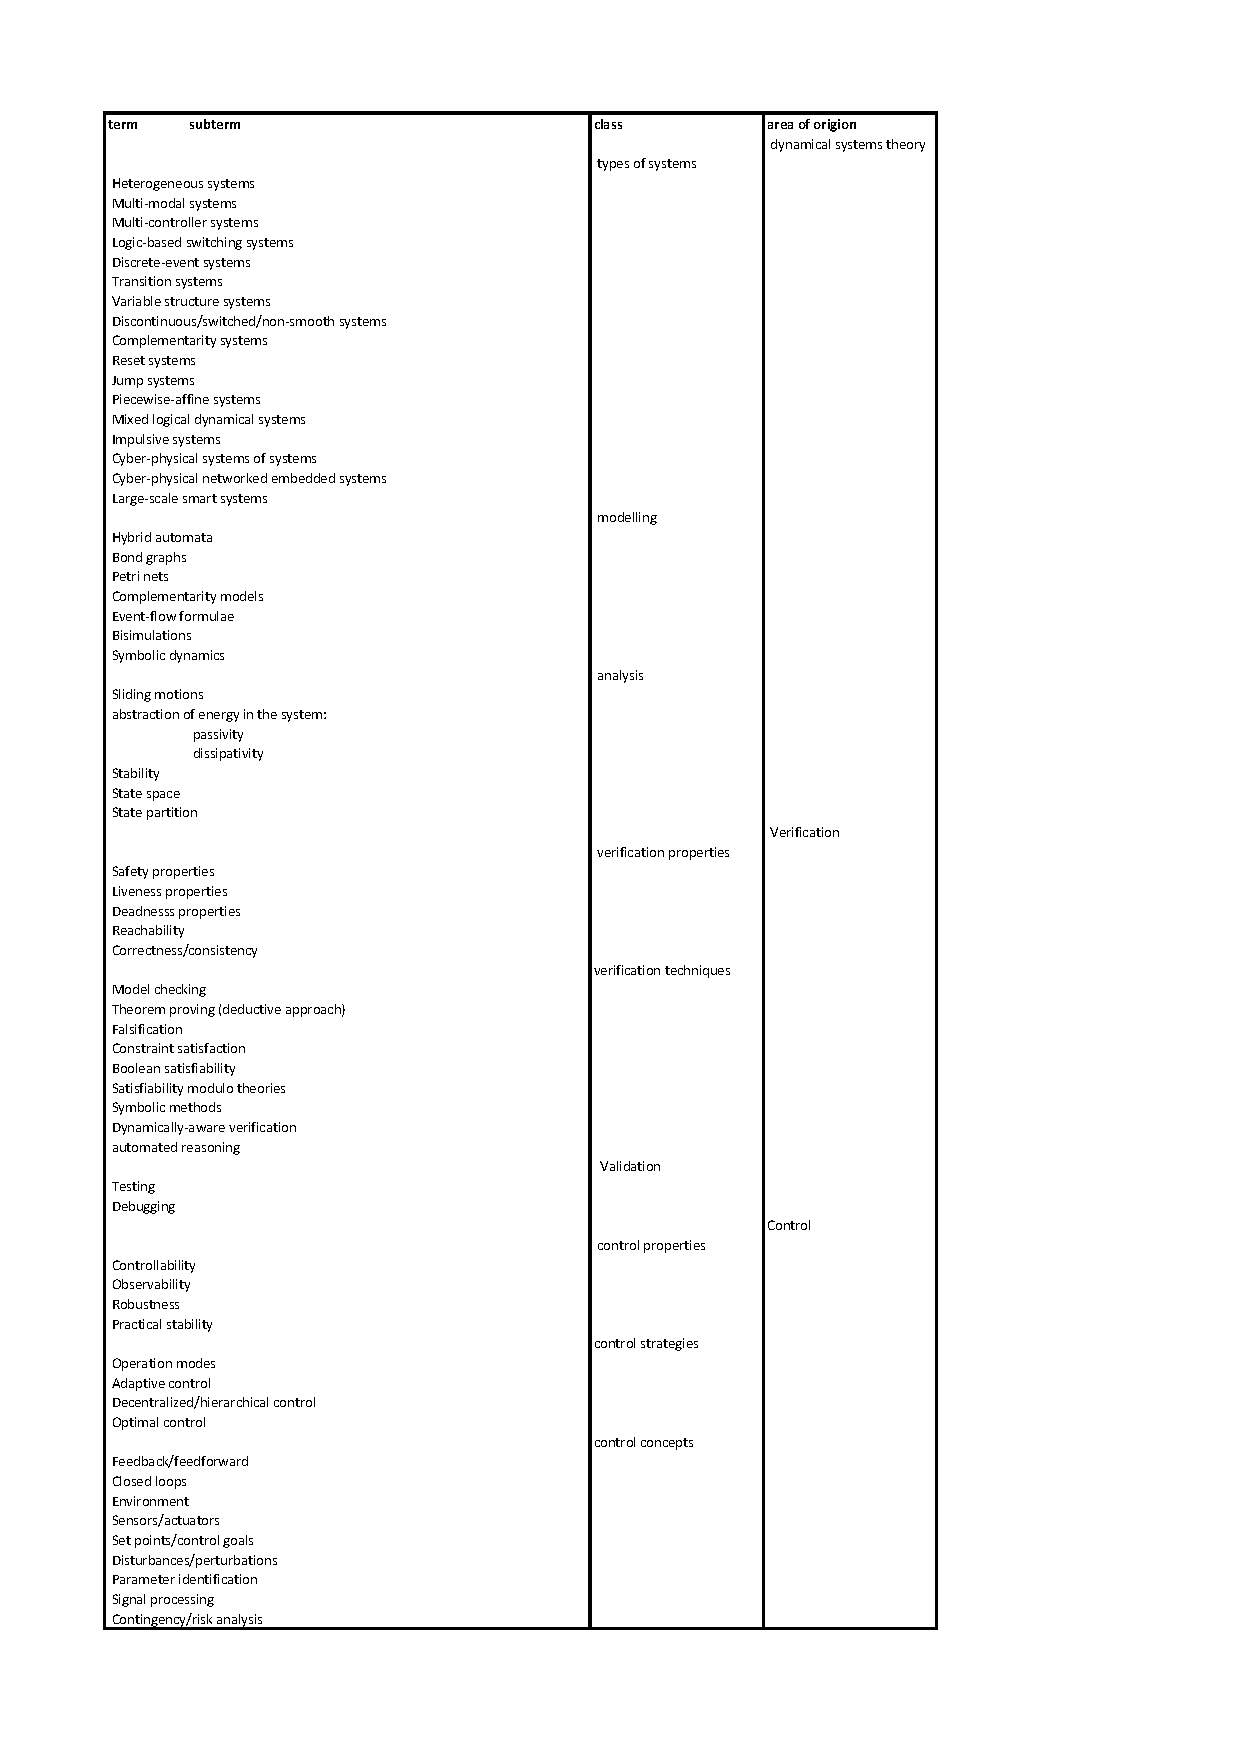
\includegraphics[width=0.7\textwidth]{figures/glossary_1.pdf}
% \caption{Terms for the glossary (1/2)}
% \label{tab:glossary_1}
% \end{table}

% \begin{table}[!htb]
% \centering
% 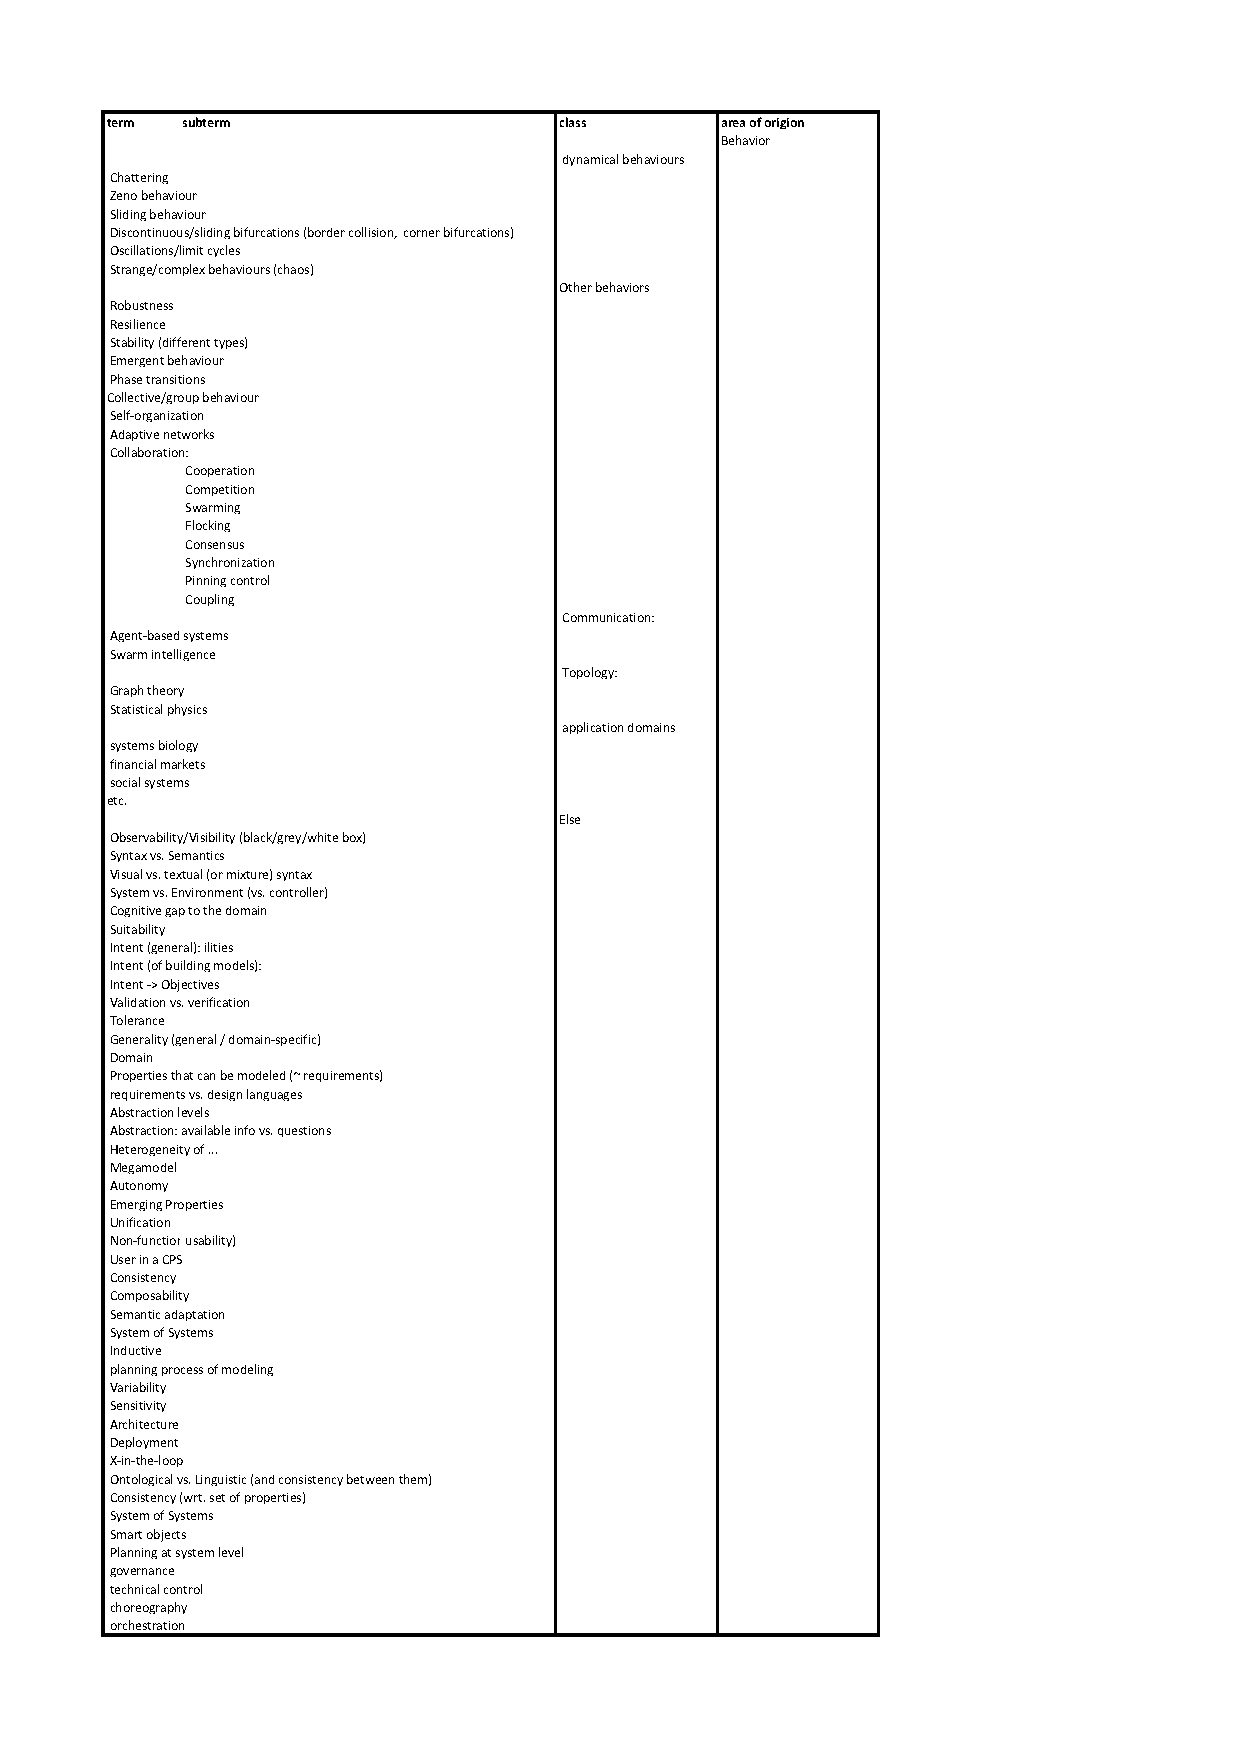
\includegraphics[width=0.7\textwidth]{figures/glossary_2.pdf}
% \caption{Terms for the glossary (2/2)}
% \label{tab:glossary_2}
% \end{table}


%\section{Term x}

\subsection{Related Terms}


% ========================================================
\chapter{Summary and Future Work}
%\todo{\textbf{TODO Holger}}
%

This report presents a catalog of formalisms, modelling languages and tools that are used in the domain of cyber-physical systems development.
It was compiled as part of the deliverables produced by the \emph{ICT COST Action IC1404 Multi-Paradigm Modelling for Cyber-Physical Systems (MPM4CPS)} -- \emph{Working Group 1 (WG1) on Foundations of MPM4CPS}.

The catalog comprises descriptions of over 170 formalisms, languages and tools, and is automatically generated from a digital ontology that was established using modern ontology engineering techniques.
The tight network of related ontology entries has been adapted to catalog form for this report.
Since it is a static snapshot of the current state of art, it requires that its contents are revisited in regular intervals to extend, update and maintain the correctness of the information.

% The second part of the report presents a glossary of terms that are commonly used in the multi-paradigm modelling and cyber-physical systems domains.
% It is intended for novice users and can be used to avoid ambiguities, for example when interacting with stakeholders from different domains.
% It too requires the same, continuous maintenance effort that the catalog experiences.


%Future work:
% \COMMENT{ HG: Sounds to concrete and doable for the future work at the end of the COST action, or? It sounds as if we simply did not do the obvious ...}
The catalog poses a solid foundation for a future, more complete body of knowledge.
To this extent, an extension of the catalog and the addition of further, more detailed properties for all entries should be performed and the catalog extended.
Obviously, this vast and time-consuming task cannot be performed by a small group of researchers, but instead should be executed through continuous, collaborative effort.
While the descriptions and references in this catalog already provide a significant coverage of the domain, we believe that tool creators and language developers are best suited to maintain the catalog entries for their field of expertise. Evidently, this solution also requires that these experts have the means to easily create, update and alter the ontology's entries.

There also exist more concrete research tasks to be performed on the catalog.
For example, in the course of the ontology development, we discovered that there exist many more properties for each individual entry that can be used to search, filter and explore the ontology.
It would be of interest to look into possibilities of how to best represent this multi-dimensional information within a catalog, while maintaining its legibility and usability.

One possibility would be to group the entries into subsections, based on these properties.
For example, we discovered that many tools serve particular purposes, such as e.g. analysis or simulation.
This information was gathered and entered into the ontology and is readily available to be used.
At the moment, we are evaluating the benefits of this approach, as for example some tools serve multiple purposes and thus would be present in multiple subsections, thereby introducing redundancy.
The members of WG1 envisage a collaboration with experts in the ontology domains to harness their knowledge in this matter.

Future tasks should also establish links to the practical usage of the listed formalisms, tools and modelling languages. For instance, the MPM4CPS's Working Group 4 has compiled a meta-data study~\cite{barisic_wg44}, reporting on which formalisms and tools were used in primary studies of CPS modelling. 
Based on this information it can then be possible to discover e.g. common formalisms for particular CPS application domains, or e.g. list potential alternative tools and languages that can be used for certain projects. 


%ANKICA: Another direction is to understand the practical usage of the reported formalism, tools and modelling languages. For instance, as a result of the WG4 we will have a meta-data reporting on which formalism and tools were used in primary studies which report on modelling of CPS. Based on this meta-data it is possible  to perform analysis and understand in which CPS application domains certain tools were used / or for modelling which part of CPS.  



\begin{comment}

In this report on the State-of-the-art on Current Formalisms used in Cyber-Physical
Systems Development of Working Group1 (WG1) on Foundations of the ICT COST
Action IC1404 Multi-Paradigm Modelling for Cyber-Physical Systems (MPM4CPS), we
first presented 
%
a catalog of languages, formalisms, and tools in chapter
\ref{ch:catalog}. 
%
Then a glossary of terms for Cyber Physical Systems has been
presented in chapter \ref{ch:glossary}.

Both the catalog and glossary still need to be improved as future work. For the catalog, the documentation of each entry and the completeness 
of the catalog still have to be improved. In addition, the three main categories of languages, formalisms and tools of the catalog better populated, reviewed, and updated to reflect the finer classification provided by the ontology from which they are generated.
%
Finally, the presented glossary of terms for Cyber-Physical Systems is currently still 
incomplete and has to be reworked to cover all relevant terms and be better linked to 
the ontologies. 

%\todo[inline]{ Holger:\\
%LATER:\\
%- agree on consistent referencing of %figures, sections, chapters, ...\\
%- agree on UK or US English and do a %related grammar and spell checking %...\\
%}

% Appendices start here
%\appendix

% An example appendix
%\include{ExampleAppendix}
\end{comment}

% ========================================================
% Bibliography starts here
\backmatter

% Generate bibliography
\fancyhead[LO]{Bibliography}
\bibliographystyle{include/files/CE-bibtex}
\label{ch:bib} %label to refer to
\bibliography{bibliography} 


~\newpage
% ========================================================
% Index starts here
%
\fancyhead[LO]{Index}
\addcontentsline{toc}{chapter}{Index}
\printindex

\BLOCK{
~\newpage
% ========================================================
% List of todos starts here
%
\listoftodos
}

\end{document}

